% \iffalse meta-comment
%
% Copyright (C) \the\year by Liu Benyuan <liubenyuan@gmail.com>
% This file may be distributed and/or modified under the
% conditions of the LaTeX Project Public License, either
% version 1.2 of this license or (at your option) any later
% version. The latest version of this license is in:
%
% http://www.latex-project.org/lppl.txt
%
% and version 1.2 or later is part of all distributions of
% LaTeX version 1999/12/01 or later.
%
% \fi
%
% \iffalse
% <package>\NeedsTeXFormat{LaTeX2e}[1999/12/01]
% <package>\ProvidesPackage{nudtpaper}
% <package>[2020/07/01 v2.8 By Liu Benyuan <liubenyuan@gmail.com>]
%<*driver>
\ProvidesFile{nudtpaper.dtx}[2020/07/01 v2.8 NUDT]
\documentclass[11pt]{ltxdoc}
\usepackage{nudtx}
\EnableCrossrefs
\CodelineIndex
\RecordChanges
\begin{document}
  \DocInput{\jobname.dtx}
\end{document}
%</driver>
% \fi
%
% \def\thuthesis{\textsc{Thu}\-\textsc{Thesis}}
% \def\nudtpaper{\textsc{Nudt}\-\textsc{Paper}}
%
% \CheckSum{1480}
% \CharacterTable
%  {Upper-case    \A\B\C\D\E\F\G\H\I\J\K\L\M\N\O\P\Q\R\S\T\U\V\W\X\Y\Z
%   Lower-case    \a\b\c\d\e\f\g\h\i\j\k\l\m\n\o\p\q\r\s\t\u\v\w\x\y\z
%   Digits        \0\1\2\3\4\5\6\7\8\9
%   Exclamation   \!     Double quote  \"     Hash (number) \#
%   Dollar        \$     Percent       \%     Ampersand     \&
%   Acute accent  \'     Left paren    \(     Right paren   \)
%   Asterisk      \*     Plus          \+     Comma         \,
%   Minus         \-     Point         \.     Solidus       \/
%   Colon         \:     Semicolon     \;     Less than     \<
%   Equals        \=     Greater than  \>     Question mark \?
%   Commercial at \@     Left bracket  \[     Backslash     \\
%   Right bracket \]     Circumflex    \^     Underscore    \_
%   Grave accent  \`     Left brace    \{     Vertical bar  \|
%   Right brace   \}     Tilde         \~}
%
% \changes{v0.99}{2009/08/12}{Initial Release}
%
% \GetFileInfo{\jobname.dtx}
%
% \DoNotIndex{\begin,\end,\begingroup,\endgroup}
% \DoNotIndex{\ifx,\ifdim,\ifnum,\ifcase,\else,\or,\fi}
% \DoNotIndex{\let,\def,\xdef,\newcommand,\renewcommand}
% \DoNotIndex{\expandafter,\csname,\endcsname,\relax,\protect}
% \DoNotIndex{\Huge,\huge,\LARGE,\Large,\large,\normalsize}
% \DoNotIndex{\small,\footnotesize,\scriptsize,\tiny}
% \DoNotIndex{\normalfont,\bfseries,\slshape,\interlinepenalty}
% \DoNotIndex{\hfil,\par,\hskip,\vskip,\vspace,\quad}
% \DoNotIndex{\centering,\raggedright}
% \DoNotIndex{\c@secnumdepth,\@startsection,\@setfontsize}
% \DoNotIndex{\ ,\@plus,\@minus,\p@,\z@,\@m,\@M,\@ne,\m@ne}
% \DoNotIndex{\@@par,\DeclareOperation,\RequirePackage,\LoadClass}
% \DoNotIndex{\AtBeginDocument,\AtEndDocument}
%
% \IndexPrologue{\section*{索引}%
%    \addcontentsline{toc}{section}{索~~~~引}}
% \GlossaryPrologue{\section*{修改记录}%
%    \addcontentsline{toc}{section}{修改记录}}
%
% \renewcommand{\abstractname}{摘~~要}
% \renewcommand{\contentsname}{目~~录}
%
% \title{\textsc{NUDTpaper:}\,\,NUDT研究生学位论文\LaTeX{}模板使用手册\thanks{NUDT \LaTeX{} Thesis Template}}
% \author{刘本源 \\ \texttt{Liubenyuan@gmail.com}}
% \date{\fileversion\ (\filedate)}
%
% \maketitle
% \thispagestyle{empty}
%
% \begin{abstract}
% 本模板旨在提供规范的国防科技大学\LaTeX{}写作模板环境,
% 现支持硕士/博士学位论文格式,可以自动生成盲评、制作A3封面。
% \end{abstract}
%
% \vspace{2cm}
% \def\abstractname{免责声明}
% \begin{abstract}\noindent
% \begin{enumerate}
% \item 本模板的发布遵守 \LaTeX{} Project Public License,使用前请认真阅读协议内容
% \item 本模板创立参照官方严格的论文写作手册,并同时参照硕士/博士学位论文\textbf{doc}文档对比修改
% \item 国防科技大学对论文写作提供写作指南与官方\textbf{doc}模板,
% 同时提供官方的\LaTeX{}模板,本模板的出发点是方便大家使用专业的高效的论文书写工具,
% 其有点在于注重排版质量、命令规范、使用方便、更新及时,符合论文撰写说明。
% 但任何由于使用本模板而引起的论文格式审查问题均与本模板作者无关。
% \item 任何个人或组织均可以本模板为基础进行修改、扩展,生成新的专用模板,但请严格遵
% 守\LaTeX{} Project Public License 协议
% \item 欢迎提出修改意见
% \end{enumerate}
% \end{abstract}
%
% \clearpage
% \tableofcontents
%
% \clearpage
% \pagenumbering{arabic}
% \pagestyle{mainpage}
%
% \section{快速上手}
% \begin{description}
% \item[安装\TeX] 下载最新的\TeX{}live或者C\TeX{}并安装
% \item[字体] 用户需要具备\verb|simsun.ttf|, \verb|simhei.ttf|, \verb|simkai.ttf|,
% \verb|STZHONGS.TTF|, 上述字体都是windows自带的; 除此之外,在网上搜索(或者C\TeX{}
% 论坛)``Adobe Opentype 中文字体'',一搜一大把,确保下载下来Adobe的四款OTF字体:
% 宋,黑,仿宋,楷体。Linux用户可将上述字体复制到\verb|/usr/share/fonts/TTF|下。
% 最新更新:用户可以考虑使用方正字体生成更为漂亮(颜色深均匀)的论文排版。
% 这三个选项分别为\verb|ttf|、\verb|otf|和\verb|fz|。
% \item[试一试] 解压缩下载的模板,双击makepdf.bat(祈祷一下),如果生成了
% \verb|thesis.pdf|$\rightarrow$
% \item[那么我的那些常用的包都在么?] 你会想我的{\bf Trans}论文可以无缝
% 的复制过来么? 对于这一点,你可以修改\verb|mynudt.sty|来实现。但是{\hei 注意},大部分包
% 都在模板中了,而且{\hei 切记切记},不要擅自改动字体等版面设计,我们继续看$\rightarrow$
% \item[咦,数学公式不是很美观呀] 笔者{\hei 强烈}建议用户使用{\bf mtpro2}宏包的,怎么使用,
% 又有哪些好处,参见bookzh.sty吧!不会错的。好了,我们专注于内容本身吧$\rightarrow$
% \item[开始写了] 所有文件均采用UTF8编码,因此要保证你的\TeX{}编辑器
% (winedt, texworks, texmaker, vim, 记事本($\cdots{}$)等)支持这种编码,
% (经过一番搜索设置后)打开\verb|thesis.tex|,如果看到的是中文$\rightarrow$
% \item[漫长的写作] 手边准备着\LaTeX{}的常用帮助文档(数学,图表,引用等),
% 结合你喜欢的文献管理软件(JabRef等), 漫长的\texttt{编辑,编译,修改,编辑,
% 编译$\cdots$}过程之后,突然有一天发现你写完了$\rightarrow$
% \item[校订] 经过老师师兄师弟师妹齐心协力校正之后,你所做的只是:
% \texttt{生成明评论文,制作明评封面,生成盲评论文,制作盲评封面},
% 装订,上交$\rightarrow$
% \end{description}
% {\color{magenta} Done!}
%
% \section{模板介绍}
%
% \textsc{NUDTpaper} 旨在帮助并且推广\LaTeX{}在国防科技大学论文中的应用,
% 本文将尽可能帮助用户掌握\textsc{NUDTpaper}的安装方法,
% 如果仍旧有不清晰的地方可以参考样例文件或者
% 给作者邮件\footnote{liubenyuan@gmail.com},感兴趣的同学可以帮忙维护模板,
% 这个模板首先符合官方的设计要求,希望同学们在使用后能够提出你们的修改意见。
% 该模板很大程度上参考了6院黄老师sofoot的国防科大博士论文模板,
% 哈工大的\LaTeX{}模板以及清华的Thuthesis
% \footnote{主页:\url{http://thuthesis.sourceforge.net}},
% 有很多使用的帮助、\verb|.cls|中的命令以及版面设置均来自Thuthesis和sofoot的模板,
% 对此的引用表示感谢。
%
% {\color{blue}\fs 模板的作用在于减轻论文写作过程中格式调整的时间,
% 其前提就是遵守模板的用法,不提倡手动更改格式,不建议正文中使用
% 手动调节版面的命令,尤其禁止修改行距和使用\verb|\normalsize|,
% 否则即使使用了\textsc{NUDTpaper}也难以保证输出的论文符合学校规范。}
%
% \section{安装}
% \label{sec:install}
%
% \subsection{下载}
% \textsc{NUDTpaper} 主页:\url{http://github.com/liubenyuan/nudtpaper}。
% 模板的更新信息发布在\href{http://github.com/liubenyuan/nudtpaper/release}{Ctex论坛}。
% \nudtpaper{}的开发版本同样可以在\textsc{gitorious}上获得。
%
% \subsection{模板的组成部分}
% 下表列出了 \nudtpaper{} 的主要文件及其功能介绍,学习模板的最好办法
% 就是参考thesis.pdf!
% \begin{center}
% \begin{longtable}{l|p{8cm}}
% \toprule
% {\hei 文件(夹)} & {\hei 功能描述}\\\midrule
% \endfirsthead
% \toprule
% {\hei 文件(夹)} & {\hei 功能描述}\\\midrule
% \endhead
% \endfoot
% \endlastfoot
% nudtpaper.ins & 模板驱动文件 \\
% nudtpaper.dtx & 模板文档代码的混合文件\\
% nudtpaper.cls & 模板类文件\\
% nudtpaper.cfg & 模板配置文件\\
% thesis.bib & 参考文献样式文件\\
% \hline
% mynudt.sty & 在这里添加你自己的宏包 \\
% thesis.tex & 示例文档主文件\\
% ref/ & 示例文档参考文献目录\\
% data/ & 示例文档章节具体内容\\
% figures/ & 示例文档图片路径\\
% \textbf{nudtpaper.pdf} & 用户手册(本文档)\\
% \textbf{thesis.pdf} & 示例文档 \\
% \bottomrule
% \end{longtable}
% \end{center}
%
% \subsection{\TeX{}系统的选择}
% 有网络环境的用户推荐安装\href{http://www.tug.org/texlive}{\TeX{}live},
% \href{http://miktex.org}{MiKTeX}或者\href{http://www.ctex.org}{C\TeX},
% 对于无网络环境的,主要是针对教研室用户,推荐{\TeX{}live}或者C\TeX{}完整版,安装
% 过程很简单,一路下一步即可,但是需要\textbf{注意:}
%
% \begin{description}
% \item[字体] TTF选项默认调用Windows系统字体,其中楷体、仿宋需要安装Office;OTF选项需要
% Adobe的商业字体(可以使你的论文更加漂亮!),这些中文字体(宋,黑,仿宋,楷体)可以从
% \href{http://dl.getdropbox.com/u/857066/adobe_chinese_otf.7z}{这里下载},
% 如果上述链接不能使用,请搜索\textsc{Adobe Opentype 中文字体}自行下载。
% 英文字体使用Windows自带。起始更推荐几款Times(Arial)类似的OTF英文字体,可以使用
% 更多排版、段落的字体特性。
% \item[粗宋] 模板中在需要宋体加黑的地方需要使用\textbf{华文中宋}, 即STZHONGS.TTF。
% \item[xeCJK] 无网络环境中,C\TeX{}完整版和\TeX{}live最新版都包括了需要的xeCJK版本。
% \end{description}
%
% \subsection{使用模板}
% \label{sec:install-cls}
% {\hei 注:默认的发行版本已经包含了可以使用的模板环境,
% 包括编译好的cls以及论文样例源文件,
% 想快速上手的话,可以直接参看\verb|thesis.tex|,进行修改。
% 写作的过程就是将你的论文的内容放到\verb|data|文件夹中,
% 图片放到\verb|figures|文件夹中,用\textsc{jabref}修改\verb|thesis.bib|即可。}
%
% 当用户需要编译生成自己的PDF版论文时,需要依次输入如下命令(注意了,如果不是使用nomencl,
% 则无需使用第二个命令)。
%
% 若使用biber,则命令为:
% \begin{shell}
% $ xelatex thesis
% $ # makeindex -s nomencl.ist -o thesis.nls thesis.nlo
% $ biber thesis
% $ xelatex thesis
% $ xelatex thesis
% \end{shell}
%
% 若使用bibtex,则命令为:
% \begin{shell}
% $ xelatex thesis
% $ # makeindex -s nomencl.ist -o thesis.nls thesis.nlo
% $ bibtex thesis
% $ xelatex thesis
% $ xelatex thesis
% \end{shell}
%
% 而为了简化用户使用,模板中提供了快捷脚本文件:
% \begin{shell}
% # 下面命令可以直接生成thesis.pdf,你可能只需要这步
% C:\> makepdf.bat
% # linux用户可以直接使用makefile
% $ make pdf
% \end{shell}
% 现在,就要进入激动人心的写作过程了。
%
% \section{使用说明}
% \label{sec:how-to-use}
% 首先,一篇论文(电子信息工程专业为例),主要的构成就是
% 封面导言,正文,表格,图片,公式,
% 交叉引用及文献索引这五部分,下面将分别详细讲解。
%
% \label{sec:howtoask}
% 在开始之前,先问自己几个问题:
% \begin{compactenum}
% \item 我是不是已经掌握了 \LaTeX{} 基础知识?
% \item 我是不是认真地阅读了模板文档?
% \item 周围有没有同学可以帮我?
% \end{compactenum}
% 更推荐用户去阅读示例文档的源代码,改写会给你一个快速的开始。
%
% \subsection{示例文件}
% \label{sec:example}
% 该示例文件是顶层的文件,包括论文属性设置、章节的安排、参考文献附录等。
% 细节用户可以参考\verb|thesis.tex|和\verb|data/|文件夹。
%
% \subsubsection{模板选项}
%
% 论文的第一句话是调用模板:
% \changes{v2.0}{2010/11/10}{增加盲评的说明}
%
%    \begin{macrocode}
%<thesis>%1. 规范硕士导言
%<thesis>% \documentclass[master,ttf]{nudtpaper}
%<thesis>%2. 规范博士导言
%<thesis>% \documentclass[doctor,twoside,ttf]{nudtpaper}
%<thesis>%3. 建议使用OTF字体获得较好的页面显示效果
%<thesis>%   OTF字体从网上获得,各个系统名称统一。
%<thesis>%   如果你下载的是最新的(1201)OTF英文字体,建议修改nudtpaper.cls,使用
%<thesis>%   Times New Roman PS Std
%<thesis>% \documentclass[doctor,twoside,otf]{nudtpaper}
%<thesis>%   另外,新版的论文模板提供了方正字体选项FZ,效果也不错哦
%<thesis>% \documentclass[doctor,twoside,fz]{nudtpaper}
%<thesis>%4. 如果想生成盲评,传递anon即可,仍需修改个人成果部分
%<thesis>% \documentclass[master,otf,anon]{nudtpaper}
%<thesis>%
%<thesis>%5. 参考文献若用biblatex生成,则使用biber选项
%<thesis>% \documentclass[master,biber]{nudtpaper}
%<thesis>%
%<thesis>%6. 简历中的论文和成果用biblatex参考文献方式生成,则使用resumebib选项
%<thesis>% \documentclass[master,biber,resumebib]{nudtpaper}
%<thesis>%
%    \end{macrocode}
%    \begin{macrocode}
%<*thesis>
\documentclass[doctor,twoside,biber,resumebib,fz]{nudtpaper}
\usepackage{mynudt}

%</thesis>
%    \end{macrocode}
%
% 模板的参数设置(开关)描述见:
%
%\begin{description}
%\item[master,doctor]
% 硕士论文用master,博士论文就用doctor
%\item[twoside]
% 指定论文为单面打印还是双面打印,当使用\verb|twoside|选项之后,
% 论文会将章节开在奇数页右手边,默认为\verb|openany|单面打印。
%\item[ttf,otf]
% 决定使用何种字体,TTF默认使用Windows自带的字体,而OTF则使用Adobe的字体(需要下载),
% TTF字体的优势是满足学校论文对于字体的要求,缺点是制作出来的PDF文件在浏览时可能发虚,
% 而OTF字体屏幕显示饱满,而且字体有很多选项可以方便\XeTeX{}排版。推荐使用\textbf{otf}
% 选项。不论何种选项,都需要安装宋体中宋(STZHONGSONG)字体(Windows自带)。
%\item[anon]
% 是否为盲评版本,如需盲评,请加上anon。
%\item[biber]
% 是否利用biblatex生成参考文献,若使用biblatex,则加上biber选项,若适用bibtex,则去除该选项。
%\item[resumebib]
% 是否利用biblatex生成简历中成果,若使用biblatex,则加上resumebib选项,否则去除该选项。
%\end{description}
%
% 如果需要使用自己定义的命令、宏包,请放于\verb|mynudt.sty|中。
% 事实上,该文件中已经添加了很多有用的宏包和命令,你可以参照修改。
% 这些之所以没有放到模板中,一则为了简洁,二则赋予用户在格式之外更多的自由。
% 里面的宏包有:代码高亮、算法环境、向量命令等,请仔细查看。
%
% 样例文件默认的是硕士论文(master),OTF字体(otf)。
%
% \subsubsection{封面导言}
% 官方模板中设计论文题目、作者等信息可以跟填空一样完成:
%
% \begin{description}
% \item[论文封头]
% 主要有四部分内容,中图分类号,学号,论文密级和UDC。
% 密级分为:\textbf{秘密} 或者 \textbf{公开}。
%    \begin{macrocode}
%<*thesis>
\classification{TP957}
\serialno{0123456}
\confidentiality{公开}
\UDC{}
%</thesis>
%    \end{macrocode}
%
% \item[论文题目,作者,日期]
% 分别包括中文和英文两部分,由于论文题目可能超过1行,
% 我们提供额外的一个命令\verb|\displaytitle|用来在
% 授权书中填入(限定为)单行的题目; 中文日期需要中文输入大写,英文日期为月年,
% 在论文最终完成后,请\textbf{手动}设定日期。
% \changes{v2.5}{2015/05/11}{修改英文作者和导师的格式,姓大写}
% \changes{v2.5}{2015/05/11}{英文导师前缀为Prof.}
%
%    \begin{macrocode}
%<*thesis>
\title{国防科大学位论文\LaTeX{}模板\\
使用手册}
\displaytitle{国防科技大学学位论文\LaTeX{}模板}
\author{张三}
\zhdate{\zhtoday}
\entitle{How to Use the \LaTeX{} Document Class for NUDT Dissertations}
\enauthor{ZHANG San}
\endate{\entoday}
%</thesis>
%    \end{macrocode}
%
% \item[论文分类及其他]
% 主要是作者的学科类别,研究方向,导师信息等。
% 每一项都包括中英文信息:
%
%    \begin{macrocode}
%<*thesis>
\subject{通信与信息工程}
\ensubject{Information and Communication Engineering}
\researchfield{自动目标识别与模糊工程}
\supervisor{李四\quad{}教授}
\cosupervisor{王五\quad{}副教授} % 没有就空着
\ensupervisor{Prof. LI Si}
\encosupervisor{} % 没有就空着
\papertype{工学}
\enpapertype{Engineering}
%</thesis>
%    \end{macrocode}
%
% \item[中英文摘要]
% 论文中需要写中文以及英文摘要,页码为小写罗马字母,关键字为黑体,
% 英文关键字为\verb|Arial|,
% 模板中定义了相关环境\verb|\cabstract|以及\verb|\eabstract|来书写摘要,
% 以及\verb|\ckeywords|以及\verb|\ekeywords|来写关键字。
% 建议用户将摘要单独放在在\verb|abstract.tex|文件中,
% 在正文中\verb|\begin{cabstract}
%% 简述背景
%随着云计算环境下各种技术的快速发展和应用,给人类生活带来巨大便利的同时也引发了人们对于数据隐私安全的关注。聚类算法以其易用性和可扩展性广泛用于各种数据挖掘研究和应用中。
%%指出隐私安全问题
%云计算在赋能海量数据上聚类应用的同时,也带来了数据泄漏的风险。目前聚类方面的隐私保护相关研究大力发展,但是仍存在一些问题。
%%具体问题描述
%%方案难以兼顾效率与安全
%一方面,目前关于隐私保护聚类的相关研究难以兼顾效率与安全,完全安全的方案通常效率较低耗时较长,无法在实际环境中应用。运行开销较小,耗时较短的方案则通常存在数据安全问题,例如泄漏中间结果,或者是数据分布信息。
%%对于聚类其他算法的研究较少
%另一方面,当前隐私保护聚类相关研究主要基于K-means,该算法包含的复杂计算较少,流程简单,但应用场景与效果都有局限性。聚类包含许多不同类型的实现,例如谱聚类、密度聚类、核聚类等,分别有其适用的场景和优点,在隐私计算的场景下相关研究相对较少。
%
%% 因此提出了我们的方案
%本文深入分析了当前云环境下隐私保护聚类方案中存在的问题,以兼顾安全与高效为目标,设计了能够实现隐私保护的k-means聚类、密度聚类等方案。本文的主要工作与贡献如下:

%聚类的应用以及存在的问题
聚类作为一种无监督机器学习算法,广泛用于数据挖掘与特征提取等研究领域,影响着人们生活的方方面面。随着数据量的迅速增加,面向大数据的聚类算法对金融行业中的股票投资分析、商业环境中的市场营销分析以及医疗领域的影像分析都具有重要应用价值。然而,一方面,随着移动手机、可穿戴设备以及各种智能设施的广泛使用,用于聚类分析的数据量呈现爆炸性增长的趋势;另一方面,当下许多应用场景要求联合多方数据进行聚类以提升数据分析的质量,对聚类的方式提出了更多的要求。

%云计算的应用,存在的问题
云计算以开放的标准和服务为基础,提供安全、快捷、便利的数据存储和网络计算服务,具有成本低、效率高、灵活性强和高可扩展性等优点。越来越多公司、机构和独立用户选择将数据存储到云平台上,运行聚类算法获取数据分类的结果。
%在数据挖掘分析技术的发展过程中,基于海量丰富的数据样本和可靠多样的聚类算法,云计算以其强大的计算和存储资源,灵活的服务方式,为大数据上的聚类应用发展提供了坚实的基础。
云计算凭借其强大的计算和存储资源,以及灵活的服务方式,为大数据上的聚类应用提供了坚实的基础。
然而,数据安全问题始终是阻碍云计算进一步推广和应用的主要因素之一。用户将未经处理的数据上传到云平台,即失去了对数据的有效控制,用户数据可能在存储和处理的过程中被拦截、篡改或传播,带来巨大的数据泄露风险。为了解决上述问题,通常采取数据加密后上传的方式来保护数据的安全性,但是加密后的数据在聚类过程中的可用性大大降低。因此,如何在云环境下大数据上进行安全高效的聚类,成为我们面临的重大挑战,也受到学术界以及工业界的广泛关注和研究。

本文深入分析云计算中聚类应用所面临的安全问题,基于数据挖掘中广泛应用的K-means聚类和密度聚类算法开展隐私保护问题的关键技术研究。

本文的主要研究内容和贡献包含如下几个方面:
\begin{compactenum}
%兼顾效率与安全的隐私保护k-means聚类
\item 针对外包计算中隐私保护K-means聚类方案中存在的数据安全和效率问题,本文提出了一种基于Kd-tree的隐私保护外包K-means聚类方案。
首先,用户在本地数据的基础上构造Kd-tree,然后通过秘密共享的方式上传至云平台,两个云服务器通过执行一系列高效的安全计算协议获取最终结果。
一方面,方案借助Kd-tree数据结构加速聚类划分的过程,减少冗余计算,提升了算法运行效率;另一方面,基础安全计算协议可以迁移到基于秘密共享的隐私计算场景中,具备良好的扩展性。实验验证表明,本方案不仅有效保障了用户数据的安全性,同时也实现了高效精准的外包K-means聚类。

%隐私保护DBSCAN聚类相关研究
\item 针对密度聚类(Density-Based Spatial Clustering Applications with Noise,DBSCAN),本文设计了三种隐私保护方案。首先,基于DBSCAN设计了全新的隐私保护计算协议,引入临时簇的概念,通过记录相连信息来还原聚类结果,在提升安全性的前提下,运行效率相较于同类工作提升近100倍。其次,为解决DBSCAN聚类结果不稳定的问题,设计了一个能够获取稳定划分结果的改进隐私保护协议,在牺牲一定性能的情况下,显著提升了聚类结果的质量,运行效率较同类工作提升近20倍。最后,针对重要参数依赖人工分析数据分布进行设置的问题,给出了一种基于DBSCAN的隐私保护层次聚类方法,借助k线图和k近邻算法获取关键参数,能够在包含不同密度数据的数据集上较好的进行聚类。经过全面的对比实验与分析,证明上述三个方案能够在保护原始信息、中间结果以及聚类结果数据安全的同时,高效的完成聚类。   
\end{compactenum}                                               
\end{cabstract}
\ckeywords{云计算;隐私保护聚类;秘密共享;安全多方计算}

\begin{eabstract}
As an unsupervised machine learning algorithm, clustering is widely used in research fields such as data mining and feature extraction, affecting all aspects of people's lives. With the rapid increase of data volume, the clustering algorithm for big data has significant application value for stock investment analysis in the financial industry, marketing analysis in the business environment and image analysis in the medical field. However, on the one hand, with the widespread use of mobile phones, wearable devices, and various smart facilities, the amount of data used for cluster analysis shows an explosive growth trend; On the other hand, many application scenarios require clustering of multi-party data to improve the quality of data analysis, more requirements are placed on clustering.

Cloud computing is based on open standards and services, centered on the Internet, and provides secure, fast, and convenient data storage and network computing services, with the advantages of low cost, high efficiency, flexibility, and scalability. More and more companies, institutions, and independent users choose to store data on cloud platforms and run clustering algorithms to obtain data analysis results.
In the development process of data mining and analysis technology, based on massive and rich data samples and reliable and diverse clustering algorithms, cloud computing provides a solid foundation for the development of clustering applications on big data with its powerful computing and storage resources and flexible service methods.
%However, data security issues have always been one of the main factors hindering the further promotion and application of cloud computing, uploading unprocessed data to the cloud platform, that is, losing effective control over the data, data may be intercepted, tampered with or spread in the process of storage and processing, bringing huge data leakage risks. 
Despite the many benefits of cloud computing, one major obstacle preventing its widespread adoption is the concern surrounding data security. In uploading unprocessed data to a cloud platform, effective control over the data is lost, thereby increasing the likelihood of data interception, tampering, or unauthorized dissemination. Such risks present a significant threat to data privacy, leading to potential data leakage catastrophes.
In order to solve the above problems, the security of data is usually protected by uploading data after encryption, but the availability of encrypted data in the clustering process is greatly reduced. Therefore, how to carry out safe and efficient clustering of big data in the cloud computing environment has become a major challenge for us, and has also received extensive attention and research from academia and industry.

This paper deeply analyzes the security problems faced by clustering applications in cloud computing and conducts research on key technologies of privacy-preserving schemes based on K-means clustering and density clustering algorithms widely used in data mining. The main research content and contributions of this paper include the following aspects:

1. Aiming at the data security and efficiency problems in the privacy-preserving K-means clustering scheme in outsourced computing, this paper proposes a Kd-tree based privacy-preserving outsourcing K-means clustering scheme. First, users construct Kd-trees based on their local data, and then upload them to the cloud platform through secret sharing, and the two cloud servers obtain the final result by executing a series of efficient secure computing protocols. On the one hand, the scheme accelerates the process of clustering and division with the help of the Kd-tree data structure, reduces redundant calculation, and improves the operational efficiency of the algorithm. On the other hand, the basic secure computing protocol can be migrated to the secure computing scenario based on secret sharing, which has good scalability. Theoretical analysis and experimental verification show that this scheme not only provides complete data security but also realizes efficient and accurate outsourced K-means clustering.

2. Three privacy-preserving schemes are designed for Density-Based Spatial Clustering Applications with Noise (DBSCAN). Firstly, we design a novel privacy-preserving DBSCAN scheme and the concept of temporary cluster is introduced. The clustering results are restored by recording the connected information and the operation efficiency is nearly 100 times higher than that of the similar scheme under the premise of improving security. 
Secondly, to solve the problem of unstable DBSCAN clustering results, an improved privacy-preserving protocol is designed which can obtain stable and high-quality clustering results at the expense of certain performance. The operation efficiency is nearly 20 times higher than that of the similar research work. 
Finally, in view of the problem that important parameters rely on manual analysis of data distribution for setting, a privacy-preserving hierarchical clustering method based on DBSCAN is proposed, and key parameters are obtained with the help of k line plot and knn algorithm, which has better performance on datasets containing data of different densities. After comprehensive experimental and theoretical analysis, it is proved that these schemes can efficiently complete clustering while protecting the security of original data and intermediate results.   
\end{eabstract}
\ekeywords{Cloud Computing, Privacy-Preserving Clustering, Secret Sharing, Secure Multiparty Computation}

|即可。其格式为:
%
% \begin{example}
% \begin{cabstract}
% 中文摘要
% \end{cabstract}
% \ckeywords{关键字}
%
% \begin{eabstract}
% Abstract
% \end{eabstract}
% \ekeywords{Key}
% \end{example}
% \end{description}
%
% \subsubsection{框架构成}
%
% 在定义完论文元素之后,就可以开始写论文正文了。用\LaTeX{}写论文的文件目录构成
% 可以很随意,模板中将图形文件单独放到一个目录中\verb|figure|中,论文正文各个
% 章节置于\verb|data|中;当然也以以\verb|chapter|为目录。
%\changes{v2.2}{2011/05/27}{使用nomencl包管理符号列表}
%\changes{v2.2}{2011/07/08}{默认使用nomencl管理参考文献}
%\changes{v2.2}{2011/09/10}{回复原先使用的denotation方式添加符号列表}
%
% 如果使用nomencl制作符号列表,在文档开始前要加入\verb|\makenomenclature|命令
% 默认还是使用denotation的方式。nomencl可以参考第二章相关章节,而denote方式
% 请参考\verb|data/denotation.tex|文件(简单的列表环境)。
%
%<thesis>% 加入makenomenclature命令可用nomencl制作符号列表。
%
%    \begin{macrocode}
%<*thesis>

\begin{document}
\graphicspath{{figures/}}
%</thesis>
%    \end{macrocode}
% 制作完封面后就是正文四大部分了,分别为:
%
% \begin{compactenum}
% \item frontmatter: 生成目录,图目录,表目录
% \item midmatter: 摘要,符号列表
% \item mainmatter: 正文,致谢,文献,成果
% \item backmatter: 附录
% \end{compactenum}
%
%<thesis>% 制作封面,生成目录,插入摘要,插入符号列表 \\
%<thesis>% 默认符号列表使用denotation.tex,如果要使用nomencl \\
%<thesis>% 需要注释掉denotation,并取消下面两个命令的注释。 \\
%<thesis>% cleardoublepage% \\
%<thesis>% printnomenclature% \\
%
%    \begin{macrocode}
%<*thesis>
\maketitle
\frontmatter
\tableofcontents
\listoftables
\listoffigures

%<thesis>%如果不是送审论文,则将true改为false即可
\newif\ifreview\reviewfalse

\midmatter
\begin{cabstract}
%% 简述背景
%随着云计算环境下各种技术的快速发展和应用,给人类生活带来巨大便利的同时也引发了人们对于数据隐私安全的关注。聚类算法以其易用性和可扩展性广泛用于各种数据挖掘研究和应用中。
%%指出隐私安全问题
%云计算在赋能海量数据上聚类应用的同时,也带来了数据泄漏的风险。目前聚类方面的隐私保护相关研究大力发展,但是仍存在一些问题。
%%具体问题描述
%%方案难以兼顾效率与安全
%一方面,目前关于隐私保护聚类的相关研究难以兼顾效率与安全,完全安全的方案通常效率较低耗时较长,无法在实际环境中应用。运行开销较小,耗时较短的方案则通常存在数据安全问题,例如泄漏中间结果,或者是数据分布信息。
%%对于聚类其他算法的研究较少
%另一方面,当前隐私保护聚类相关研究主要基于K-means,该算法包含的复杂计算较少,流程简单,但应用场景与效果都有局限性。聚类包含许多不同类型的实现,例如谱聚类、密度聚类、核聚类等,分别有其适用的场景和优点,在隐私计算的场景下相关研究相对较少。
%
%% 因此提出了我们的方案
%本文深入分析了当前云环境下隐私保护聚类方案中存在的问题,以兼顾安全与高效为目标,设计了能够实现隐私保护的k-means聚类、密度聚类等方案。本文的主要工作与贡献如下:

%聚类的应用以及存在的问题
聚类作为一种无监督机器学习算法,广泛用于数据挖掘与特征提取等研究领域,影响着人们生活的方方面面。随着数据量的迅速增加,面向大数据的聚类算法对金融行业中的股票投资分析、商业环境中的市场营销分析以及医疗领域的影像分析都具有重要应用价值。然而,一方面,随着移动手机、可穿戴设备以及各种智能设施的广泛使用,用于聚类分析的数据量呈现爆炸性增长的趋势;另一方面,当下许多应用场景要求联合多方数据进行聚类以提升数据分析的质量,对聚类的方式提出了更多的要求。

%云计算的应用,存在的问题
云计算以开放的标准和服务为基础,提供安全、快捷、便利的数据存储和网络计算服务,具有成本低、效率高、灵活性强和高可扩展性等优点。越来越多公司、机构和独立用户选择将数据存储到云平台上,运行聚类算法获取数据分类的结果。
%在数据挖掘分析技术的发展过程中,基于海量丰富的数据样本和可靠多样的聚类算法,云计算以其强大的计算和存储资源,灵活的服务方式,为大数据上的聚类应用发展提供了坚实的基础。
云计算凭借其强大的计算和存储资源,以及灵活的服务方式,为大数据上的聚类应用提供了坚实的基础。
然而,数据安全问题始终是阻碍云计算进一步推广和应用的主要因素之一。用户将未经处理的数据上传到云平台,即失去了对数据的有效控制,用户数据可能在存储和处理的过程中被拦截、篡改或传播,带来巨大的数据泄露风险。为了解决上述问题,通常采取数据加密后上传的方式来保护数据的安全性,但是加密后的数据在聚类过程中的可用性大大降低。因此,如何在云环境下大数据上进行安全高效的聚类,成为我们面临的重大挑战,也受到学术界以及工业界的广泛关注和研究。

本文深入分析云计算中聚类应用所面临的安全问题,基于数据挖掘中广泛应用的K-means聚类和密度聚类算法开展隐私保护问题的关键技术研究。

本文的主要研究内容和贡献包含如下几个方面:
\begin{compactenum}
%兼顾效率与安全的隐私保护k-means聚类
\item 针对外包计算中隐私保护K-means聚类方案中存在的数据安全和效率问题,本文提出了一种基于Kd-tree的隐私保护外包K-means聚类方案。
首先,用户在本地数据的基础上构造Kd-tree,然后通过秘密共享的方式上传至云平台,两个云服务器通过执行一系列高效的安全计算协议获取最终结果。
一方面,方案借助Kd-tree数据结构加速聚类划分的过程,减少冗余计算,提升了算法运行效率;另一方面,基础安全计算协议可以迁移到基于秘密共享的隐私计算场景中,具备良好的扩展性。实验验证表明,本方案不仅有效保障了用户数据的安全性,同时也实现了高效精准的外包K-means聚类。

%隐私保护DBSCAN聚类相关研究
\item 针对密度聚类(Density-Based Spatial Clustering Applications with Noise,DBSCAN),本文设计了三种隐私保护方案。首先,基于DBSCAN设计了全新的隐私保护计算协议,引入临时簇的概念,通过记录相连信息来还原聚类结果,在提升安全性的前提下,运行效率相较于同类工作提升近100倍。其次,为解决DBSCAN聚类结果不稳定的问题,设计了一个能够获取稳定划分结果的改进隐私保护协议,在牺牲一定性能的情况下,显著提升了聚类结果的质量,运行效率较同类工作提升近20倍。最后,针对重要参数依赖人工分析数据分布进行设置的问题,给出了一种基于DBSCAN的隐私保护层次聚类方法,借助k线图和k近邻算法获取关键参数,能够在包含不同密度数据的数据集上较好的进行聚类。经过全面的对比实验与分析,证明上述三个方案能够在保护原始信息、中间结果以及聚类结果数据安全的同时,高效的完成聚类。   
\end{compactenum}                                               
\end{cabstract}
\ckeywords{云计算;隐私保护聚类;秘密共享;安全多方计算}

\begin{eabstract}
As an unsupervised machine learning algorithm, clustering is widely used in research fields such as data mining and feature extraction, affecting all aspects of people's lives. With the rapid increase of data volume, the clustering algorithm for big data has significant application value for stock investment analysis in the financial industry, marketing analysis in the business environment and image analysis in the medical field. However, on the one hand, with the widespread use of mobile phones, wearable devices, and various smart facilities, the amount of data used for cluster analysis shows an explosive growth trend; On the other hand, many application scenarios require clustering of multi-party data to improve the quality of data analysis, more requirements are placed on clustering.

Cloud computing is based on open standards and services, centered on the Internet, and provides secure, fast, and convenient data storage and network computing services, with the advantages of low cost, high efficiency, flexibility, and scalability. More and more companies, institutions, and independent users choose to store data on cloud platforms and run clustering algorithms to obtain data analysis results.
In the development process of data mining and analysis technology, based on massive and rich data samples and reliable and diverse clustering algorithms, cloud computing provides a solid foundation for the development of clustering applications on big data with its powerful computing and storage resources and flexible service methods.
%However, data security issues have always been one of the main factors hindering the further promotion and application of cloud computing, uploading unprocessed data to the cloud platform, that is, losing effective control over the data, data may be intercepted, tampered with or spread in the process of storage and processing, bringing huge data leakage risks. 
Despite the many benefits of cloud computing, one major obstacle preventing its widespread adoption is the concern surrounding data security. In uploading unprocessed data to a cloud platform, effective control over the data is lost, thereby increasing the likelihood of data interception, tampering, or unauthorized dissemination. Such risks present a significant threat to data privacy, leading to potential data leakage catastrophes.
In order to solve the above problems, the security of data is usually protected by uploading data after encryption, but the availability of encrypted data in the clustering process is greatly reduced. Therefore, how to carry out safe and efficient clustering of big data in the cloud computing environment has become a major challenge for us, and has also received extensive attention and research from academia and industry.

This paper deeply analyzes the security problems faced by clustering applications in cloud computing and conducts research on key technologies of privacy-preserving schemes based on K-means clustering and density clustering algorithms widely used in data mining. The main research content and contributions of this paper include the following aspects:

1. Aiming at the data security and efficiency problems in the privacy-preserving K-means clustering scheme in outsourced computing, this paper proposes a Kd-tree based privacy-preserving outsourcing K-means clustering scheme. First, users construct Kd-trees based on their local data, and then upload them to the cloud platform through secret sharing, and the two cloud servers obtain the final result by executing a series of efficient secure computing protocols. On the one hand, the scheme accelerates the process of clustering and division with the help of the Kd-tree data structure, reduces redundant calculation, and improves the operational efficiency of the algorithm. On the other hand, the basic secure computing protocol can be migrated to the secure computing scenario based on secret sharing, which has good scalability. Theoretical analysis and experimental verification show that this scheme not only provides complete data security but also realizes efficient and accurate outsourced K-means clustering.

2. Three privacy-preserving schemes are designed for Density-Based Spatial Clustering Applications with Noise (DBSCAN). Firstly, we design a novel privacy-preserving DBSCAN scheme and the concept of temporary cluster is introduced. The clustering results are restored by recording the connected information and the operation efficiency is nearly 100 times higher than that of the similar scheme under the premise of improving security. 
Secondly, to solve the problem of unstable DBSCAN clustering results, an improved privacy-preserving protocol is designed which can obtain stable and high-quality clustering results at the expense of certain performance. The operation efficiency is nearly 20 times higher than that of the similar research work. 
Finally, in view of the problem that important parameters rely on manual analysis of data distribution for setting, a privacy-preserving hierarchical clustering method based on DBSCAN is proposed, and key parameters are obtained with the help of k line plot and knn algorithm, which has better performance on datasets containing data of different densities. After comprehensive experimental and theoretical analysis, it is proved that these schemes can efficiently complete clustering while protecting the security of original data and intermediate results.   
\end{eabstract}
\ekeywords{Cloud Computing, Privacy-Preserving Clustering, Secret Sharing, Secure Multiparty Computation}


\chapter*{符号使用说明}
% 可以根据需要在chapter后加星星/去掉星星

\begin{denotation}
%\begin{table}
%	\renewcommand{\arraystretch}{1.3}
%	\centering
%	\scalebox{1.0}{
%	
%	}
%
%\end{table}
%\begin{tabular}{cl}
%	$ x_i =\{x_{i1},...,x_{im}\} $ & 维度为$ m $的数据点$ x_i $\\
%	$ C = \{c_1,...,c_m\} $& Kd-tree中每个点的中心\\
%	$ Z = \{z_1,...,z_k\} $& $ k $个候选簇\\
%	$ \langle x \rangle/\langle x \rangle^A $& $ x $在$ \mathbb{Z}_n $上的加性秘密共享值\\
%	$ \langle x \rangle^B $& $ x $在$ \mathbb{Z}_2 $上的布尔共享值\\
%	MUL & 安全乘法协议\\
%	SED & 带缩放因子的安全欧式距离计算协议\\
%	SC & 安全比较协议\\
%	SMin(S/L) & 安全极值计算协议(大数据集/小数据集)\\
%	SF & 安全过滤协议\\
%	SSORT & 安全排序协议\\
%	DIST & 安全欧式距离计算\\
%	
%\end{tabular}	                                                                                                                                                                                                                                                                                                                                                                                
\item[$ x_i $ ] 维度为$ m $的数据点$ x_i =\{x_{i}[1],...,x_{i}[m]\}  $
\item[$ C $ ] Kd-tree中每个树节点的中心$ C = \{c_1,...,c_m\}  $
\item[$ Z $ ] $ k $个候选簇$ Z = \{z_1,...,z_k\} $
%\item[$ d[i] $] 数组$ d $中第$ i $个元素
\item[$ \langle x \rangle/\langle x \rangle^A $] $ x $在$ \mathbb{Z}_n $上的加性秘密共享值
\item[$ \langle x \rangle^B $ ] $ x $在$ \mathbb{Z}_2 $上的布尔共享值
\item[$ \langle x \rangle_i $] $ i\in\{0,1\} $代表秘密共享参与方
\item[MUL] 安全乘法协议
\item[SED] 带缩放因子的安全欧式距离计算协议
\item[SC] 安全比较协议
\item[SMin(S/L)] 安全极值计算协议(大数据集/小数据集)
\item[SF] 安全过滤协议
\item[SSORT] 安全排序协议
\item[DIST] 安全欧式距离计算
\item[DBSCAN] Density-based Spatial Clustering Applications with Noise
\item[Eps/$ \epsilon $] DBSCAN算法中控制邻域半径
\item[Filter] 过滤算法
%\begin{table}[h]
%	\centering
%%	\Huge %此处写字体大小控制命令
%%	\begin{tabularx}{cl}
%%		hh&dd
%%	\end{tabularx}
%	\scalebox{1.2}{
%		\centering
%		\begin{tabular}{|ll|}
%	$ x_i =\{x_{i1},...,x_{im}\} $ & 维度为$ m $的数据点$ x_i $\\
%	$ C = \{c_1,...,c_m\} $& Kd-tree中每个点的中心\\
%	$ Z = \{z_1,...,z_k\} $& $ k $个候选簇\\
%	$ \langle x \rangle/\langle x \rangle^A $& $ x $在$ \mathbb{Z}_n $上的加性秘密共享值\\
%	$ \langle x \rangle^B $& $ x $在$ \mathbb{Z}_2 $上的布尔共享值\\
%	MUL & 安全乘法协议\\
%	SED & 带缩放因子的安全欧式距离计算协议\\
%	SC & 安全比较协议\\
%	SMin(S/L) & 安全极值计算协议(大数据集/小数据集)\\
%	SF & 安全过滤协议\\
%	SSORT & 安全排序协议\\
%	DIST & 安全欧式距离计算\\
%		\end{tabular}
%	}
%	
%\end{table}

\end{denotation}


%</thesis>
%    \end{macrocode}
%
%<thesis>%书写正文,可以根据需要增添章节; 正文还包括致谢,参考文献与成果
%\changes{v1.4}{2009/10/31}{将成果移动到参考文献之后}
%
%    \begin{macrocode}
%<*thesis>
\mainmatter
\chapter{绪论}
云计算在赋能海量数据上的聚类应用的同时,也带来了数据泄露的风险,引起人们的广泛关注。
如何在提供便捷的云计算服务的同时,保护用户的数据安全成为了当今学术研究的热门问题,极具现实意义。
本章首先介绍云环境下的聚类应用的相关背景,然后阐述设计隐私保护聚类方案的重要意义,最后总结文章主要工作内容及创新点,并给出了整体组织结构。

\section{研究背景与意义}
% 直接一把子照搬开题报告!
随着现代社会数字化的不断演进,数据使用量呈指数级增加,个人和小型组织越来越难以在内部计算机服务器上维护所有重要信息、运行大型程序和系统。为解决这些问题,云计算应运而生。自云计算在2006年被提出后,它就被认为是能够推动下一代互联网革命的技术,并迅速成为了研究领域的热门探索方向\cite{sadiku2014cloud}。
云计算既可以指在网络上提供的应用服务,也可以指数据中心中提供这些服务的硬件和系统软件,它的核心思想是,将众多用网络连接的计算资源统一管理和调度,构成一个计算资源中心向用户提供按需服务,它的运行原理和基于Web的电子邮件客户端类似,允许用户访问系统的所有功能和文件,但是无需将系统的大部分内容保存在自己的计算机上。
此外,云计算在各个领域都有广泛且深刻的应用(如图\ref{img_cloud}),例如在智能教育领域,为学生提供在线课程和为老师提供授课工具;在智慧医疗领域,为医生和患者提供远程诊疗、电子病例和医疗数据分析等功能;在商业领域,为企业组织提供电子商务、市场分析以及资源规划等功能。

\begin{figure}[htbp]
	\centering
	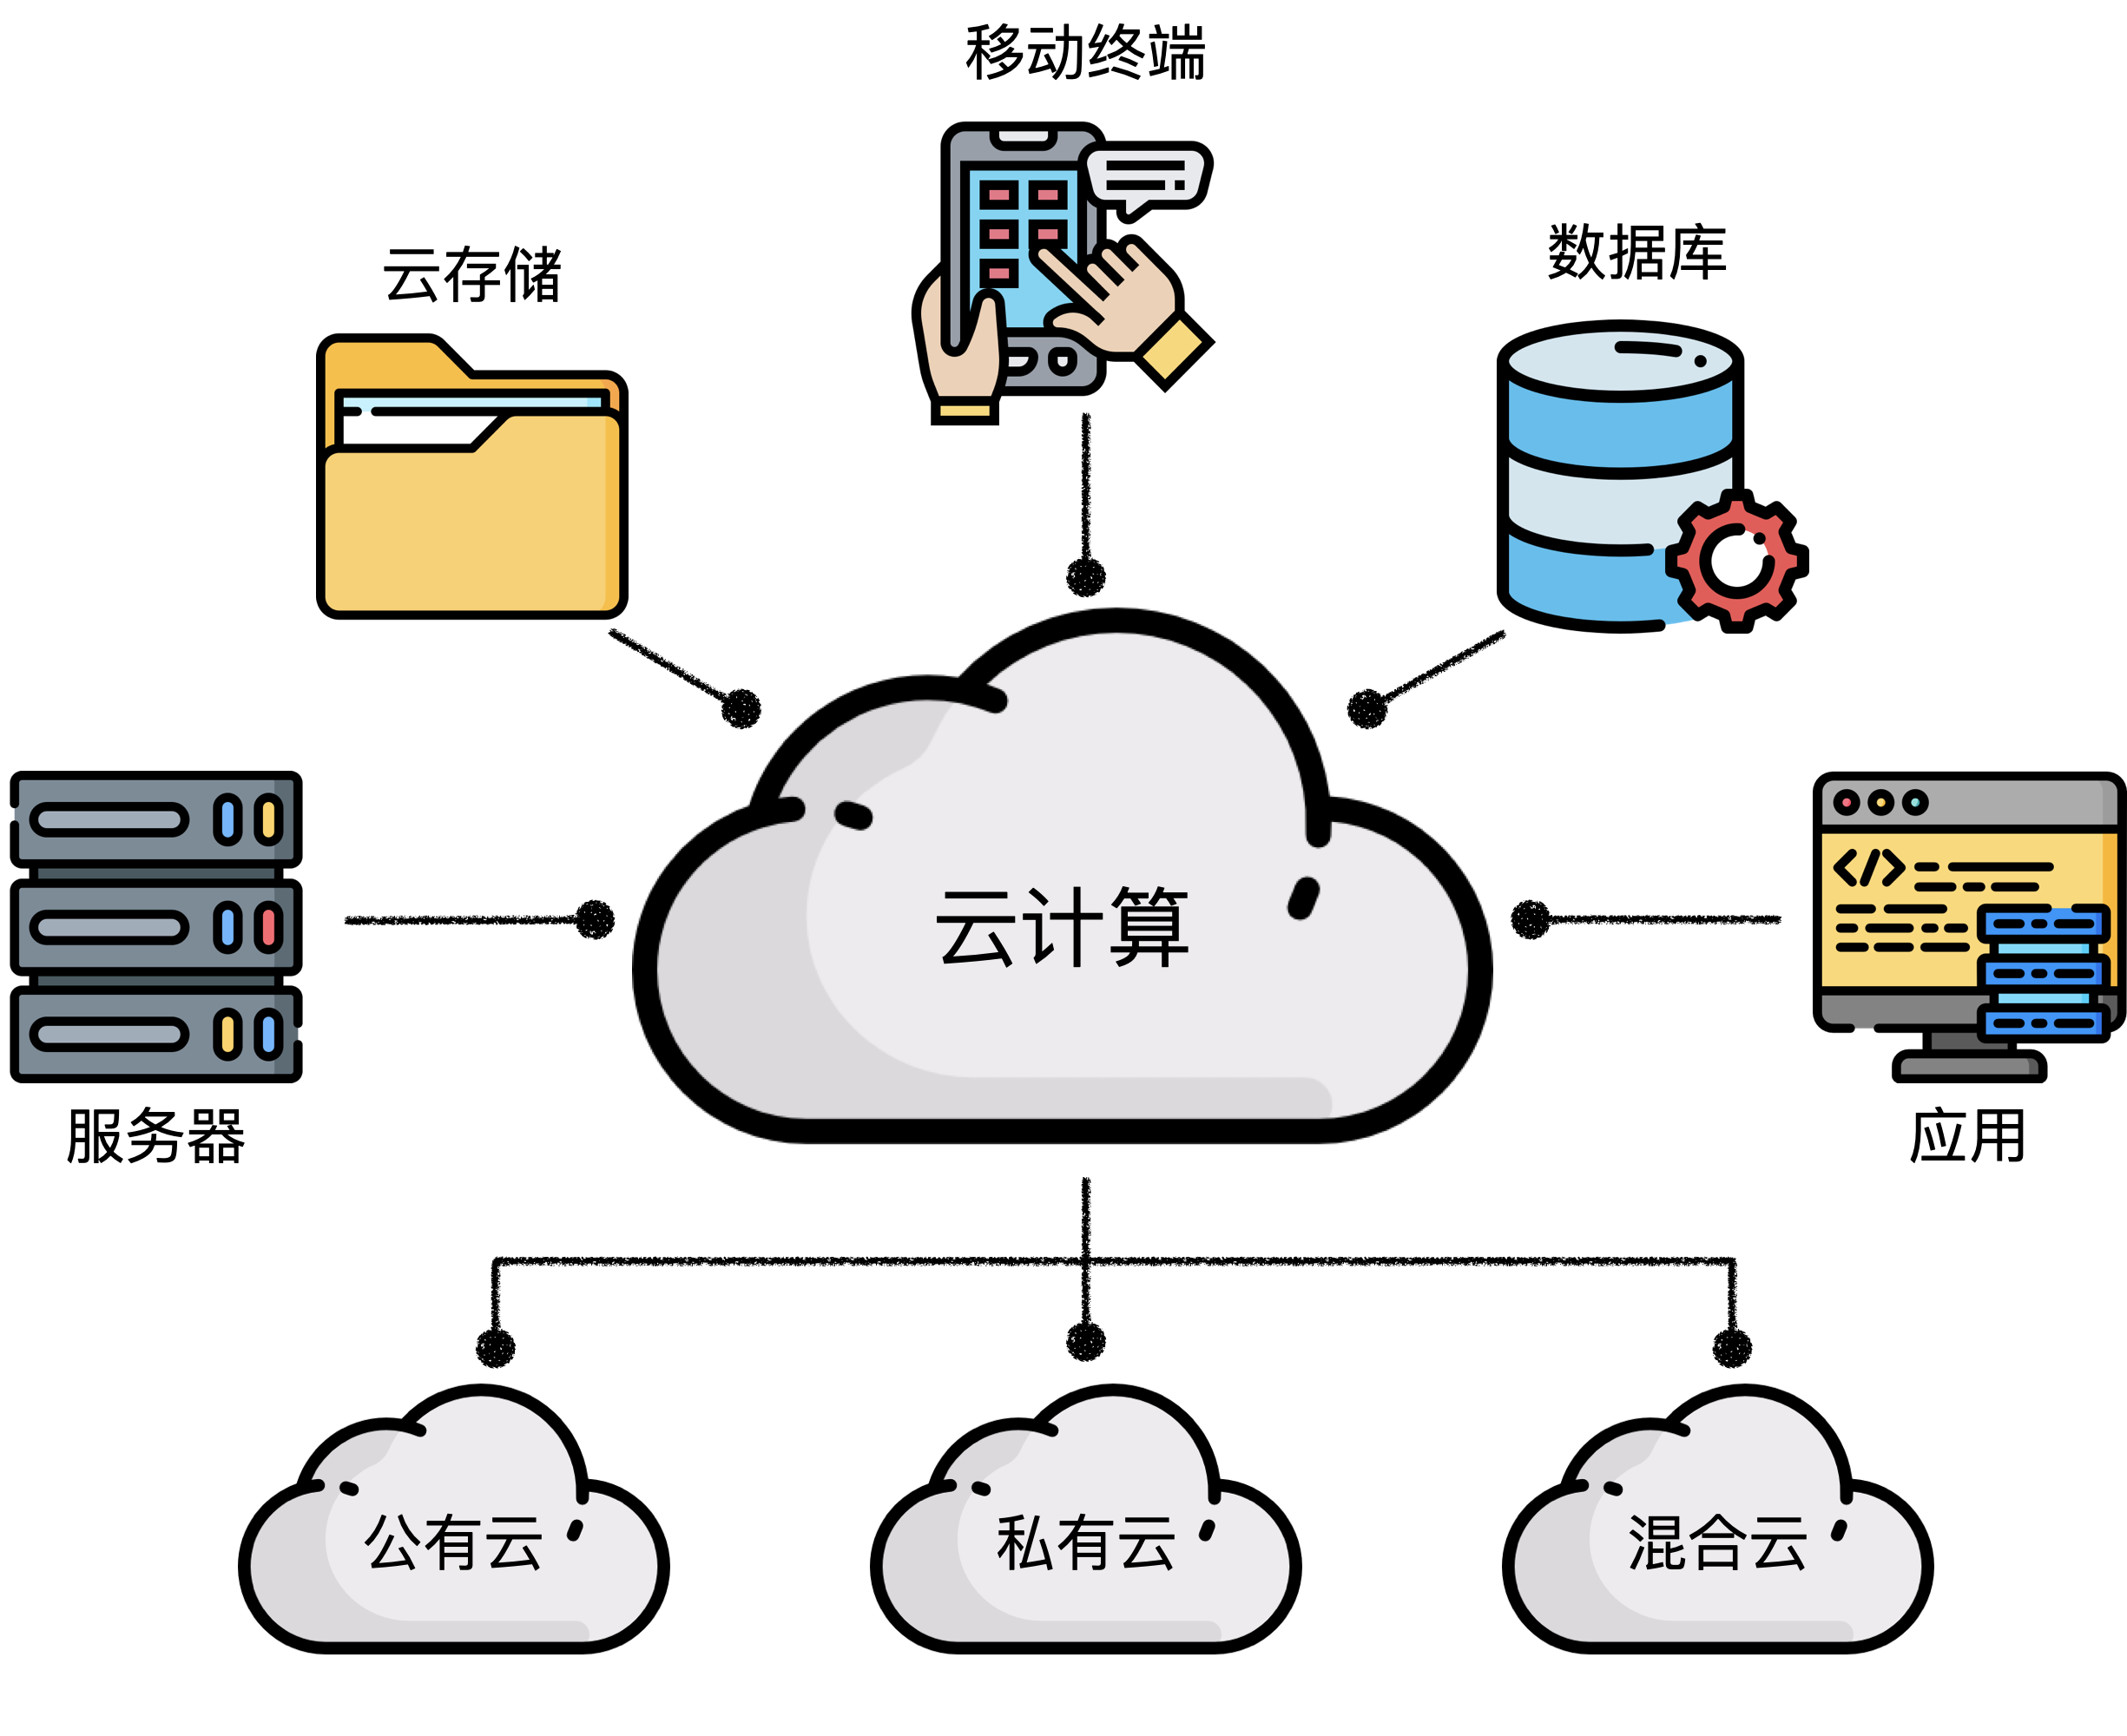
\includegraphics[width=0.55\linewidth]{img/cloudarchi.png}
	\caption{云计算架构}
	\label{img_cloud}
\end{figure}

云计算具有经济实惠、按需服务、方便、通用、多租户、灵活、稳定等特点,它主要提供了三种服务交付模式,如图\ref{img_saas}所示,分别是基础设施即服务(IaaS)、平台即服务(PaaS)、以及软件即服务(SaaS)。
IaaS将计算机硬件(例如网络存储,虚拟机,数据中心,处理器和内存)视为一种服务,无需大量资金和时间即可提供可扩展基础架构。同时,IaaS还可以用于构建防火墙,虚拟机监控和其他安全领域\cite{manvi2014resource}。
%IaaS的优势在于能够节省用户购买和维护物理设备的成本和时间,提高资源利用率和可扩展性,实现灵活的部署和迁移。常见的应用场景有网站托管、系统容灾、大数据分析以及测试开发环境等等。
PaaS以开发工具、框架、架构、程序和集成开发环境的形式提供服务。它的优势在于用户可以在云端获取各种开发工具,中间件以及数据库等资源,无需自己购买相关软硬件,关注开发的逻辑和功能即可。
%Paas的架构通常采用容器化技术,即将应用程序打包成可移植的容器,通过互联网提供给用户。但在快速发展的同时,PaaS还面临着诸多挑战,例如生命周期开发和底层基础设施安全等问题\cite{rani2014comparative}。
SaaS是远程计算服务的集合,它使得第三方供应商能够远程部署应用程序。云计算客户可以在云基础设施上通过网络获取云服务提供商的应用程序\cite{antonopoulos2010cloud}。
%SaaS的典型应用场景有办公软件、电子邮件以及企业资源规划等。其架构通常采用多租户技术,将同一套应用程序提供给多个用户使用,每个用户只能看到自己的数据和配置,提高了资源利用率和扩展性,降低了运营成本。

\begin{figure}[htbp]
	\centering
	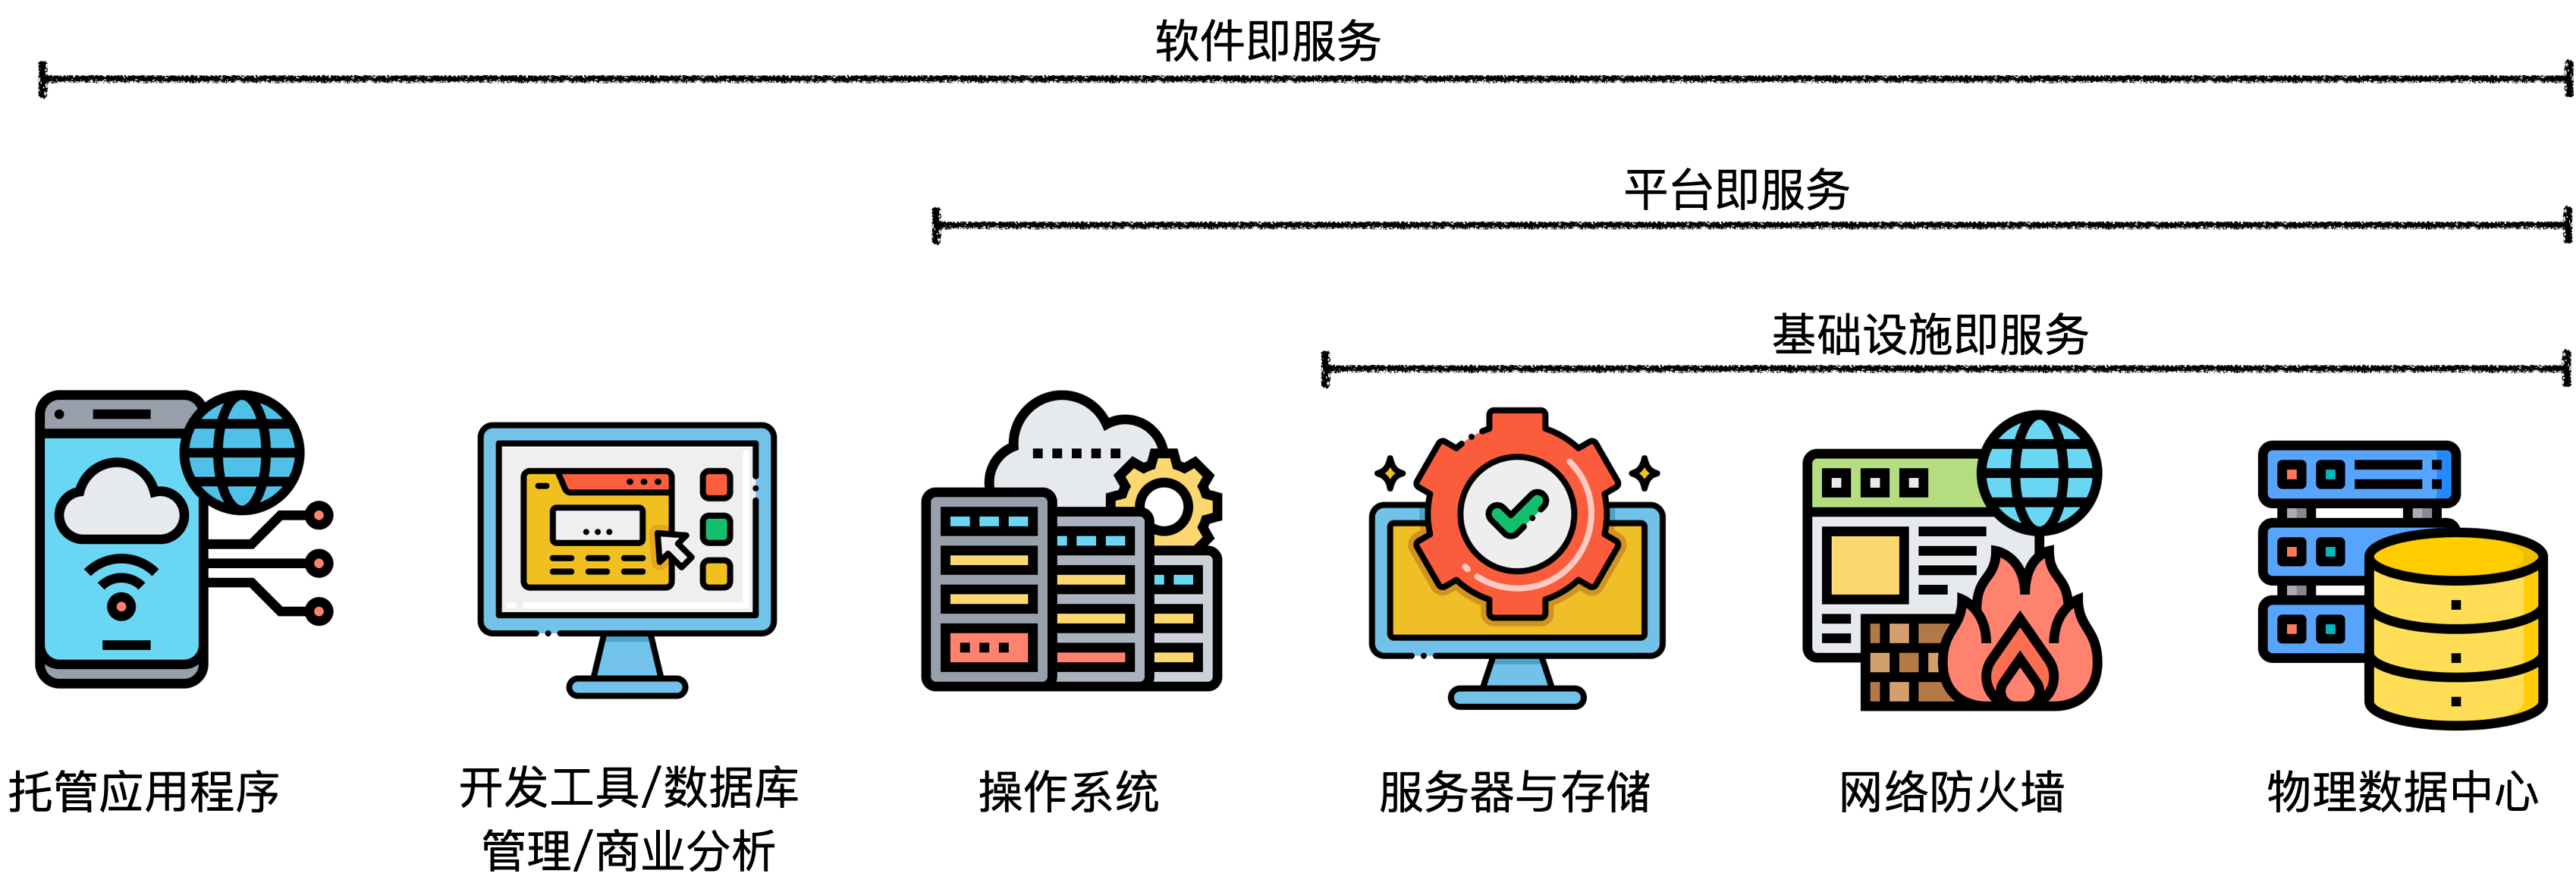
\includegraphics[width=1.0\linewidth]{img/cloudservice.png}
	\caption{云计算服务交互模式}
	\label{img_saas}
\end{figure}

近年来,云计算场景下出现了一种新的服务类型,机器学习即服务(Machine Learning as a Service,MLaaS)\cite{ribeiro2015mlaas}。随着研究的发展和设备的进步,机器学习从学术研究落地到生活的方方面面,但是大多数机器学习任务对于设备的性能要求较高,需要存储海量的数据才能取得较好的结果。大型公司有能力承担设备费用,利用机器学习的便利开展各种各样的研究与服务,但是资源有限的小公司和个人的需求常常难以被满足。

MLaaS基本上是一组基于云的工具的总称,这些工具以一种全新的方式支持科学家和数据工作者的日常工作,它们支持协作、版本控制、并行化和其他比较复杂的任务。
此外,较大的云服务供应商提供了简单明了的方法来将他们的MLaaS服务与其他工具集成,方便用户进行自动化部署以及执行机器学习任务。
MLaaS包含很多种类,例如自然语言处理、图像和视频分析、计算机视觉、语音识别以及数据挖掘等等。
随着机器学习技术的发展和进步,提供MLaaS的公司数量也在增加,主流的公司包括微软的Azure、谷歌的Google Cloud ML等等。在MLaaS中,海量的数据需要被上传到云计算中心,这一过程也被称之为外包计算。
由于用户在数据上传后失去了对数据的完全控制,因此会更加关心数据隐私问题。云计算服务模型的复杂性、实时性、数据的多元异构以及终端资源有限等特点使得传统的数据隐私保护方法无法直接用来保护云计算中的大量数据\cite{hunt2018chiron}。

在2018年,脸书被爆出隐私泄露丑闻,近5000万选民的个人资料被泄露,据称被某政治咨询公司所使用。这一丑闻的发展不仅使得该公司的市值减少数十亿美元,同时还引发了公众的强烈不满和质疑,由此可见保护数据的隐私安全无论是对公司还是对用户都有深远意义。
将一些敏感的数据进行外包以获取机器学习的结果可能会引发隐私泄漏问题,特别是在金融以及医疗领域。以医疗影像识别为例,在对数据不进行任何处理的前提下交付给云服务器进行训练,会直接造成用户私密医疗数据的泄漏,引发公众恐慌。即便是对用户的数据进行了简单的脱敏,模型训练的中间结果也可能会被恶意利用以获取信息。以K-means聚类为例,虽然原始数据经过加密,但是中间结果,例如聚类簇的大小,能够直接揭露具有某种特征的群体有多少人,以及数据的分布特点,特别有研究表明可以通过一些手段从中间结果恢复原始数据\cite{liu2021when}。因此,如何能够进行安全的外包计算,在维护用户数据安全的同时,正确的获取外包机器学习任务的结果成为一个研究热点。

聚类(Clustering)是一种非常流行的无监督机器学习技术,它能够将相似的输入元素划分到同一个簇(cluster)中。
聚类的应用领域非常广泛,从业务分析到医疗保健等诸多领域。在许多这些应用场景中,敏感信息在被正确聚类的同时,也不应该被泄漏。此外,现在经常需要将不同来源的数据组合起来进行训练以提升分析质量,庞大的数据量对资源有限的用户带来巨大的压力,因此,通常需要将复杂的计算外包给强大的云服务器进行处理,这就要求设计有效的外包隐私保护聚类方案\cite{ahmed2020k}。
目前,为了保护聚类过程中输入的敏感数据的安全性,已经有了许多研究成果,涵盖各个方面。在设计隐私保护聚类协议时,通常基于两个不同的场景,即多方计算(图\ref{scen2})与外包计算(图\ref{scen1})。
\begin{figure}[htbp] %[htbp]
	\begin{minipage}[t]{0.45\linewidth}
		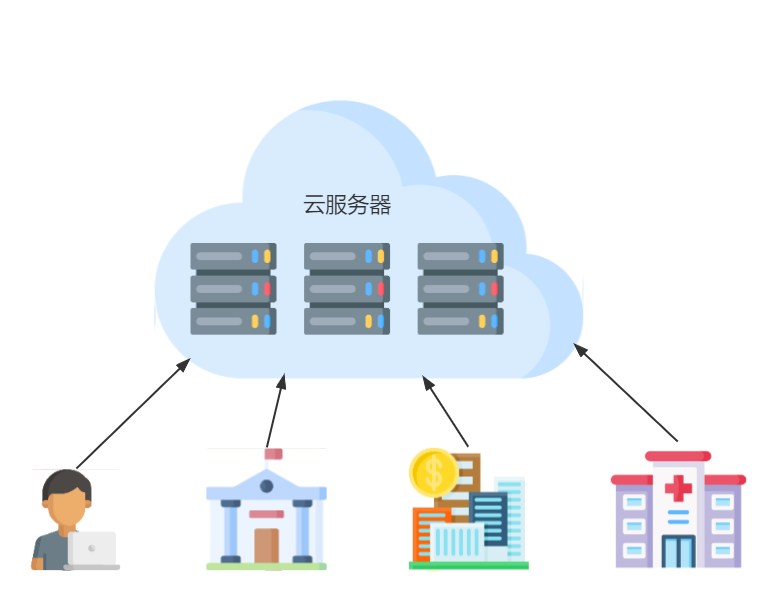
\includegraphics[width=\linewidth]{img/outsource.png}
		\caption{外包计算}
		\label{scen1}
	\end{minipage}%
	\hfill%
	\begin{minipage}[t]{0.45\linewidth}
		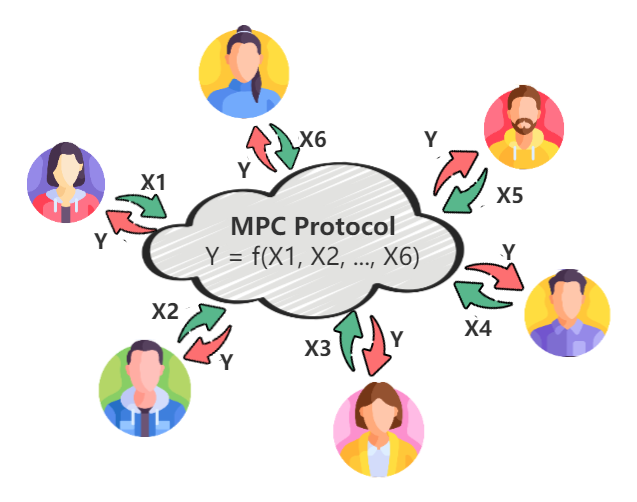
\includegraphics[width=\linewidth]{img/mpc.png}
		\caption{多方计算}
		\label{scen2}
	\end{minipage}
\end{figure}

在多方计算的场景下\cite{cramer2015secure},两个及两个以上的数据所有者共同执行安全计算协议,除了输出之外的任何内容都不会泄漏给彼此,比较常见的是两方计算。同时,一些研究也会在模型设计中引入半诚实参与方(通常是服务器)来辅助计算。
相对应的,另一种场景则是外包计算\cite{li2018privacy},一个或多个数据所有者将计算(或存储)外包给其他参与方,并假设这些参与方可以为数据所有者进行聚类而无需知道关于输入数据的任何信息。由于外包计算旨在使用外部资源,数据所有者通常不应该参与协议的执行,并处于离线状态,但是这一点通常难以完全实现。
值得一提的是,一些多方计算协议(MPC)也可以用于外包计算场景,只需要数据所有者在多个不共谋的参与方之间秘密共享自己的数据,然后多个不共谋的参与方在秘密共享数据上执行安全协议实现聚类。但是,MPC协议是否支持外包计算很大程度上取决于中间协议的设计,如果数据持有者需要在聚类过程中进行大量的明文计算或者在中间对数据进行解密,那就很难将协议转换到外包计算的场景中。

外包计算和多方计算各有其优势和缺点,对于资源有限的用户来说,外包计算更加具有实际意义和价值,能够有效的减轻用户的资源负担。基于外包计算的安全计算方法已有诸多研究,但是完全安全的聚类方案通常效率较低,即便是在性能较好的服务器上也需要花费难以接受的时间才能获得最终结果,效率较高的方案通常会牺牲一定的安全性,例如泄漏簇大小、簇中心这样的中间计算结果,带来一些隐私安全问题。因此如何设计出安全又高效的外包隐私保护聚类方案值得深入研究和探索。

综上所述,本文以云计算下的外包聚类为主要应用场景,深入分析其面临的基本问题和技术难点,以设计兼具效率与安全的方案为主要目的,针对典型的聚类算法(K-means,DBSCAN)展开研究,提出了完善的隐私保护方案,并通过理论分析和真实数据集测试,验证所述方案的安全性,高效性和正确性。通过本文的研究,期望能够为资源有限的用户提供一种可行的隐私保护外包聚类方法,为云服务提供商与独立用户提供合作的桥梁,使得用户能够专注于数据的挖掘分析,云服务提供商进一步提高资源利用率,各司其职,物尽其用,让更多人无需顾虑数据安全更加放心的享受科技进步带来的生活水平的提升。

\section{云环境下聚类中隐私保护问题概述}
%本节首先介绍聚类的概念和云环境下聚类的典型应用场景,然后讨论云环境下聚类都存在哪些具体的数据安全与隐私问题,最后讨论针对上述问题目前已有的解决方案和技术手段。
本节首先给出云环境下聚类研究综述,详细介绍了云计算、聚类算法以及云环境中聚类算法的应用,然后介绍云环境下聚类应用中存在的数据安全问题。基于上述内容,总结归纳了隐私保护聚类研究中常用的技术手段,并探讨了隐私保护聚类方案设计的目标。
\subsection{云环境下聚类相关研究概述}
%本小节首先介绍云计算的基本概念和常见应用场景,然后对机器学习中的聚类技术展开介绍,最后介绍云环境下的聚类方案基本应用。
\subsubsection{云计算概述}
云计算是指一种基于互联网的按需提供计算机系统资源,特别是数据存储(云存储)和计算能力,并且无需用户自行采购、配置或管理资源的计算模式\cite{montazerolghaem2020green},其允许用户通过互联网使用分布在世界各地的服务器上的资源。云计算的部署模型通常可以分为三种,分别是公有云、私有云和混合云。公有云由第三方云服务提供商运营,使用户可以按照特定要求和业务目标安排资源部署。私有云由单个组织构建管理,以非公开的方式托管在本地,具有更强的数据控制、安全和管理功能。混合云是上述二者的结合体,使得用户既能利用公有云服务,同时保持私有云架构中常见的安全和合规功能。

云计算具有灵活性、成本低、高可靠、以及可共享等优点,带给用户巨大的便利,资源有限的用户无需关心如何部署、管理和维护IT基础设施,只需要付费即可获取想要的资源和服务。这项技术解放了用户的双手,使他们能够专注于本领域的研究与工作,提升效率。

\subsubsection{聚类算法概述}
聚类是一种无监督机器学习算法,它能够将一组数据划分到不同的集合中,即簇。簇内部数据相似度较高,簇与簇之间数据相似度相对较低。聚类在实际的应用中非常广泛,常见于数据挖掘分析、生物信息处理、文本挖掘提取以及图像处理等领域。通过聚类能够找到不同数据集合特有的模式与结构,挖掘隐藏在背后的信息,从而进行分析和进一步处理。

常见的聚类算法包括:
\begin{compactitem}
	\item
	\textbf{基于划分的聚类方法:}也叫基于分区的聚类或基于距离的聚类,核心思想为假定数据集有$ n $个样本,在满足样本间距离的前提条件下,最少将其划分为$ k $个簇。簇内数据尽可能相似,不同簇的数据尽可能不相似。常见的基于划分的聚类方法包括K-means算法和K-medoids算法。
	\item
	\textbf{基于层次的聚类方法:}将数据对象划分为层次结构,可以采取自顶向下或者自底向上的顺序进行操作。自顶向下也称为分裂,将所有样本当作一个簇,找到最远的两个簇进行分割,直到满足预期条件。自底向上则是将每个点都看成一个独立的簇,找到距离最近的两个簇进行合并,迭代重复直到满足预期。常见的聚类算法包括AGNES、DIANA等。
	\item
	\textbf{基于密度的聚类方法:}根据样本的密度分布进行聚类,通过样本密度反映数据之间的可连接性,并通过可连接性不断扩展从而产生最终的聚类结果。算法认为密度较高的区域中数据对象属于同一个簇,密度低(包含较少或不包含数据)的区域则形成了簇的边界。该方法能够发现任意形状和大小的簇,对噪声不敏感。常见的算法有DBSCAN、OPTICS等。
	\item
	\textbf{基于网格(Grid)的聚类方法:}将数据空间划分为若干网格单元,并将数据对象映射到网格中,计算每个单元的密度,通过预设阈值来判断网格是否为高密度单元,邻近的稠密单元进行合并构成了簇。该方法可以大大减小聚类计算复杂度,但是对网格的划分方式要求较高。典型的算法包括STING、CLIQUE等。
	\item
	\textbf{基于模型的聚类方法:}该方法的核心思想为假设每个簇都符合某种概率模型,例如正态分布,然后借助最大似然估计法或者贝叶斯推断来估计模型参数并划分数据到所属簇中。该方法能够得到明确的聚类结果,但是对模型和参数的选择要求较高。常见的算法有EM、GMM等。
	%	\item \textbf{K-means:}是一种最为常见的聚类算法,基于欧式距离衡量相似度,不断迭代直到算法收敛获取划分结果。首先,随机选择$ k $个簇中心,然后遍历集合中所有数据,求解到$ k $个簇中心的距离,并据此划分到最近的簇中。最后根据划分结果,更新簇中心为簇内数据的平均值,重复上述过程直到满足判定收敛的条件。
	%	\item \textbf{层次聚类:}是通过对数据集在不同的层次进行划分,按照自顶向下或者自底向上的步骤,逐步形成树形结构的聚类算法。自底向上的方式将每一个原始数据看成一个单一的聚类,然后不断合并从而成为大的聚类。而自顶向下的方式则是将所有数据看作一个大的聚类,通过不断分割直到每一个单一数据被划分。
	%	\item \textbf{DBSCAN:}是一种典型的基于密度的聚类算法,它将簇定义为密度相连的数据点的最大集合,将满足要求的高密度区域划分为簇,能够发现任意形状的聚类,并识别噪声点,并对异常点不敏感。
\end{compactitem}

综上所述,聚类算法的划分一般可以基于划分、密度、网格和模型等方式。不同的具体聚类算法各有优缺点和适用场景。下面在表格\ref{s1_table_clustering}中,给出几个常见的聚类算法,以及它们在应用数据的规模、对噪声的抗干扰能力、适合的数据形状以及算法效率方面的特点。
\begin{table}[htbp]
	\centering
	\renewcommand{\arraystretch}{1.3}
	\caption{常见聚类算法比较}
	\label{s1_table_clustering}
	\scalebox{1.0}{
		\begin{tabular}{c|c|c|c|c}% 通过添加 | 来表示是否需要绘制竖线c|
			\hline  % 在表格最上方绘制横线
			算法类型 & 可用于大规模 & 对噪声抗干扰性 & 适合形状 & 算法效率 \\%&SKD
			\hline % 在表格最下方绘制横线
			K-means  & 是           & 较差           & 球形     & 很高     \\
			\hline
			DBSCAN   & 是           & 较好           & 任意形状 & 一般     \\
			\hline
			BIRCH    & 否           & 较差           & 球形     & 很高     \\
			\hline
			CURE     & 是           & 很好           & 任意形状 & 较高     \\
			\hline
		\end{tabular}
	}
\end{table}

本文主要基于K-means和DBSCAN聚类算法展开隐私保护方案相关研究。二者在对噪声的抗干扰性、适合的数据集形状以及算法效率方面存在一些区别。图\ref{clu_difference}中可以看到K-means和DBSCAN在不同数据集上聚类划分结果的区别,可以看到DBSCAN对于任意形状的数据集都适应的较好,而K-means则更加适合球形数据集。

\begin{figure}[htbp]
	\centering
	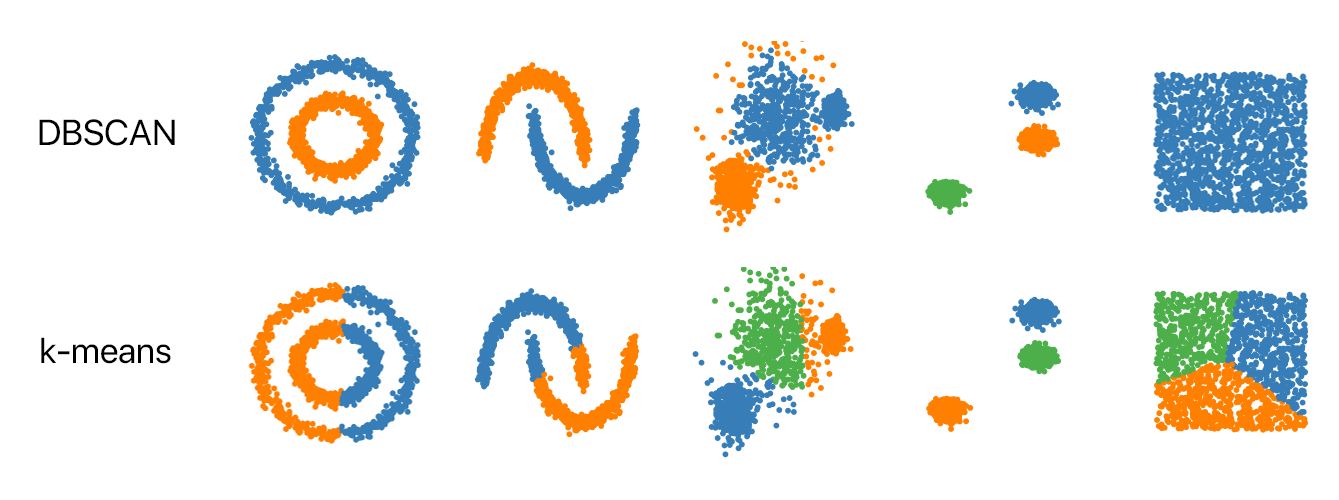
\includegraphics[width=\linewidth]{img/difference.png}
	\caption{DBSCAN与K-means聚类结果对比}
	\label{clu_difference}
\end{figure}

\subsubsection{云环境下的聚类应用}
\label{juleiyanjiu}
云环境下聚类算法的实施通常依赖于外包计算这一计算模式,即将计算任务和数据交给云服务提供商进行处理。外包计算的流程主要包括数据准备、任务分配、计算处理以及结果返回。它具有节省计算资源、提升计算效率、降低成本等优点。从用户角度来看,外包聚类计算的应用主要可以细分为两种,分别是单用户上传数据聚类,多用户分别上传数据联合聚类。

单用户外包聚类,例如高校的学生老师或是小型的研究开发团队,通常希望能够对指定的数据集进行聚类,获取结果用于后续挖掘分析。这些用户拥有的计算和通信资源通常有限,难以在本地机器上对大型数据集进行处理,因此会选择将数据上传至云平台后,以外包计算这一形式获取结果。

多用户协同外包聚类,例如银行或医院等机构,因自身业务的开展,会产生极具研究价值的数据,深入挖掘分析这些数据,可以为医疗影像研究和用户信用评估等方面的研究提供指导。然而,独立机构产生的数据量有限,海量数据上的聚类通常效果更好。因此这些机构倾向于联合其他机构,将数据上传到云平台上共同聚类。以医院为例,医疗影像常用于各种疾病的辅助诊疗,通过对这些数据进行挖掘分析能够提取出各种特征用于研究,造福人类。

综上,聚类的数据来源和形式有所区别,但算法收敛后聚类结果以相同的方式通过互联网传递回用户手中以进行后续的研究分析。
% 感觉好像并不是很必要
%两种情况,资源受限的独立用户需要外包训练,不同组织机构需要上传数据联合聚类
%聚类的实施通常需要云计算平台提供帮助与支持,尤其是在需要处理大型数据集时。本文主要考虑以下两种云环境下的聚类应用。
%
%一方面,独立用户,例如高校的学生老师或是小型的研究开发团队,他们通常希望能够对指定的数据集进行聚类,获取结果用于后续挖掘分析。这些用户通常计算资源受限,难以在本地机器上对大型数据集进行处理,因此会选择将数据上传至云平台后,以外包计算这一形式获取结果。
%
%另一方面,一些组织机构,例如银行或医院,因自身业务的开展,会产生极具研究价值的数据,深入挖掘分析这些数据,可以为医疗影像研究和用户信用评估等方面的研究提供指导。然而,独立机构产生的数据量有限,海量数据上的聚类通常效果更好。因此这些机构倾向于联合其他机构,将数据上传到云平台上共同聚类。以医院为例,医疗影像常用于各种疾病的辅助诊疗,通过对这些数据进行挖掘分析能够提取出各种特征用于研究,造福人类。
%
%综上,云环境下的聚类场景通常可以划分为两类:一种是资源受限的独立用户上传自身数据或指定开源数据集,进行聚类获取结果;另一种则是,多个用户(组织机构之间联合)上传数据到云平台联合进行聚类,获取结果以进行后续挖掘分析。
\subsection{云环境下聚类中的隐私问题}
本小节主要就云环境下外包聚类计算中存在的隐私问题展开讨论,并总结了几种现有的典型隐私保护技术。如前所述,在外包计算中,用户需要将数据全部上传至云平台,云服务器利用这些数据进行聚类训练,并回传结果。

若外包计算模式下,云平台接收的数据并非源自网络公开数据集,而是来自独立用户或者组织机构上传。在这种情况下,数据本身通常具有较高的隐私保护要求。
例如,医疗机构希望借助云计算强大的计算能力和海量的存储空间来对其医疗影像信息展开挖掘分析,从而在诊疗中辅助医生进行判断和诊断,其外包的数据通常包含患者的敏感信息,例如年龄、性别、籍贯、医疗影像以及相关医学检查结果。
智能穿戴设备需要获取用户的各种私密数据,如心率、步数、运动状态以及睡眠状态等内容进行分析然后将结果反馈给用户。
一旦发生数据泄露,会造成巨大损失。
此外,即便是对原始数据进行了加密操作,云平台在这些密文数据上进行聚类获取结果的同时,还会获取若干中间计算结果,这些数据的安全性也要纳入考虑。因此,对于云环境下隐私保护方案中数据安全的研究,需要考虑原始数据,中间结果以及划分结果等多个方面。

\subsection{隐私保护聚类技术手段}
云环境下隐私保护聚类方案的一大难点在于,如何在保证原始数据以及中间结果隐私性的前提下,完成安全高效的聚类运算。当下,聚类研究中常见的隐私保护技术手段大体上可以分为数据扰动、差分隐私、同态加密以及安全多方计算。本节将分别介绍上述几种技术的基本原理以及各自的优缺点。

\subsubsection{数据扰动}
数据扰动(Data Perturbation)是一种隐私保护方法,允许在不泄漏原始数据信息的情况下,对数据进行一定的扰动,从而达到保护隐私的目的。数据扰动方式主要可以分为两种类型:

\begin{compactitem}
	\item \textbf{概率分布方式:}是数据扰动技术中一种重要手段,通过调整数据的概率分布来保护敏感信息。通常从相同的分布样本中或者从分布本身中获取数据进行替换。常见的实现的方式有拉普拉斯机制、高斯机制以及指数机制。但是若数据分布比较复杂,则难以用简单的概率分布来进行扰动。同时噪声的大小和分布需要根据具体的应用场景和应用特征来进行选择。
	\item \textbf{数值失真方式:}借助加法、乘法或其他随机过程扰乱数据。其中,添加加性随机噪声,使得攻击者无法获取单个数据的原始信息,但是由于没有影响数据的分布特征,因此仍能够通过分析挖掘出数据相关有效信息。乘性扰动则是指利用数据投影等方法,将原始数据映射到低维空间,例如可以使用随机映射技术将数据映射到一个随机选择的子空间中。
\end{compactitem}

综上所述,数据扰动技术实施较简单,引入开销较小,适用场景广泛,但是存在着安全性较低、影响数据质量等问题。具体使用需要权衡数据隐私性和数据准确性,进行取舍。

\subsubsection{差分隐私}
Dwork等人\cite{dwork2006differential}在2006年提出一种全新的隐私定义,即差分隐私。它能够确保在数据集合中添加或者删除某项内容,不会显著影响任何相关数据分析的结果\cite{dwork2008differential},将隐私泄露风险控制在可接受范围内,恶意攻击者无法通过观察运算结果来获取精确的单个数据信息。目前已有较多关于差分隐私的研究和应用,实际场景中通常采取本地化差分隐私技术保护隐私安全,苹果的iOS系统\cite{team2017learning}、谷歌的Chrome浏览器\cite{erlingsson2014rappor}以及微软的Windows系统\cite{ding2017collecting}均已应用。
差分隐私的具体定义\cite{dwork2011firm}如下:

\begin{definition}
	设有随机算法$ \varGamma $,$ \varGamma $所有可能输出构成的集合为$ O_{\varGamma} $。对于任意两个邻近数据集$ D $和$ D' $以及$ O_{\varGamma} $的任何子集合$ S_{\varGamma} $,若算法$ \varGamma $满足
	\begin{equation}
		\operatorname{Pr}\left[M(D) \in S_M\right] \leq \exp (\varepsilon) \times \operatorname{Pr}\left[M\left(D^{\prime}\right) \in S_M\right]
	\end{equation}
	则称算法$ \varGamma $ 能够提供$ \epsilon -$差分隐私保护。
\end{definition}

其中参数$ \epsilon $称为隐私保护预算,它用来控制算法$ \varGamma $在两个相邻数据集上取得相同输出的概率比值,反映了$ \varGamma $提供的隐私保护水平,当$ \epsilon $越小时,隐私保护的力度越大,需要的噪声越多,$ \epsilon $等于0时,隐私保护水平最高。

通过在原始数据上添加噪声,既保护了隐私又保留了原始数据的统计特征。以数据库查询为例,利用差分隐私技术对数据库进行处理,实现了数据库中具体某个记录发生变化但不影响数据发布的结果,同时攻击者无法通过观察数据库发布的结果来推测用户的某条记录是否在数据库中,进而实现隐私保护。

使用差分隐私技术能够有效避免数据泄露,保护用户的隐私,通过控制添加噪声的多少,可以在数据的隐私保护与查询结果的准确性之间取得一定的平衡。此外,差分隐私对于数据的保护能力不受具体数据特征的影响,能够用于各种类型的数据和场景。然而差分隐私技术存在一定的局限性,在处理较小数据集时,添加噪声的影响变大,可能会导致数据质量下降,进而影响数据挖掘分析的结果。引入差分隐私,会带来计算和时间成本,降低系统的效率。

综上,差分隐私既有隐私保护能力,又有其受限制的地方,需要结合实际应用场景的特点来选择性使用。

\subsubsection{同态加密}
同态加密(Homomorphic Encryption)是由Rivest,Adleman和Dertouzos\cite{rivest1978data}于1978年首次提出,Craig Gentry\cite{gentry2009fully}于2009年首次实现的一种加密方法。
在Gentry提出一个可行的全同态加密方案之前,同态加密的发展时间线\cite{acar2018survey}如下图\ref{timeline}所示。

\begin{figure}[htbp]
	\centering
	%	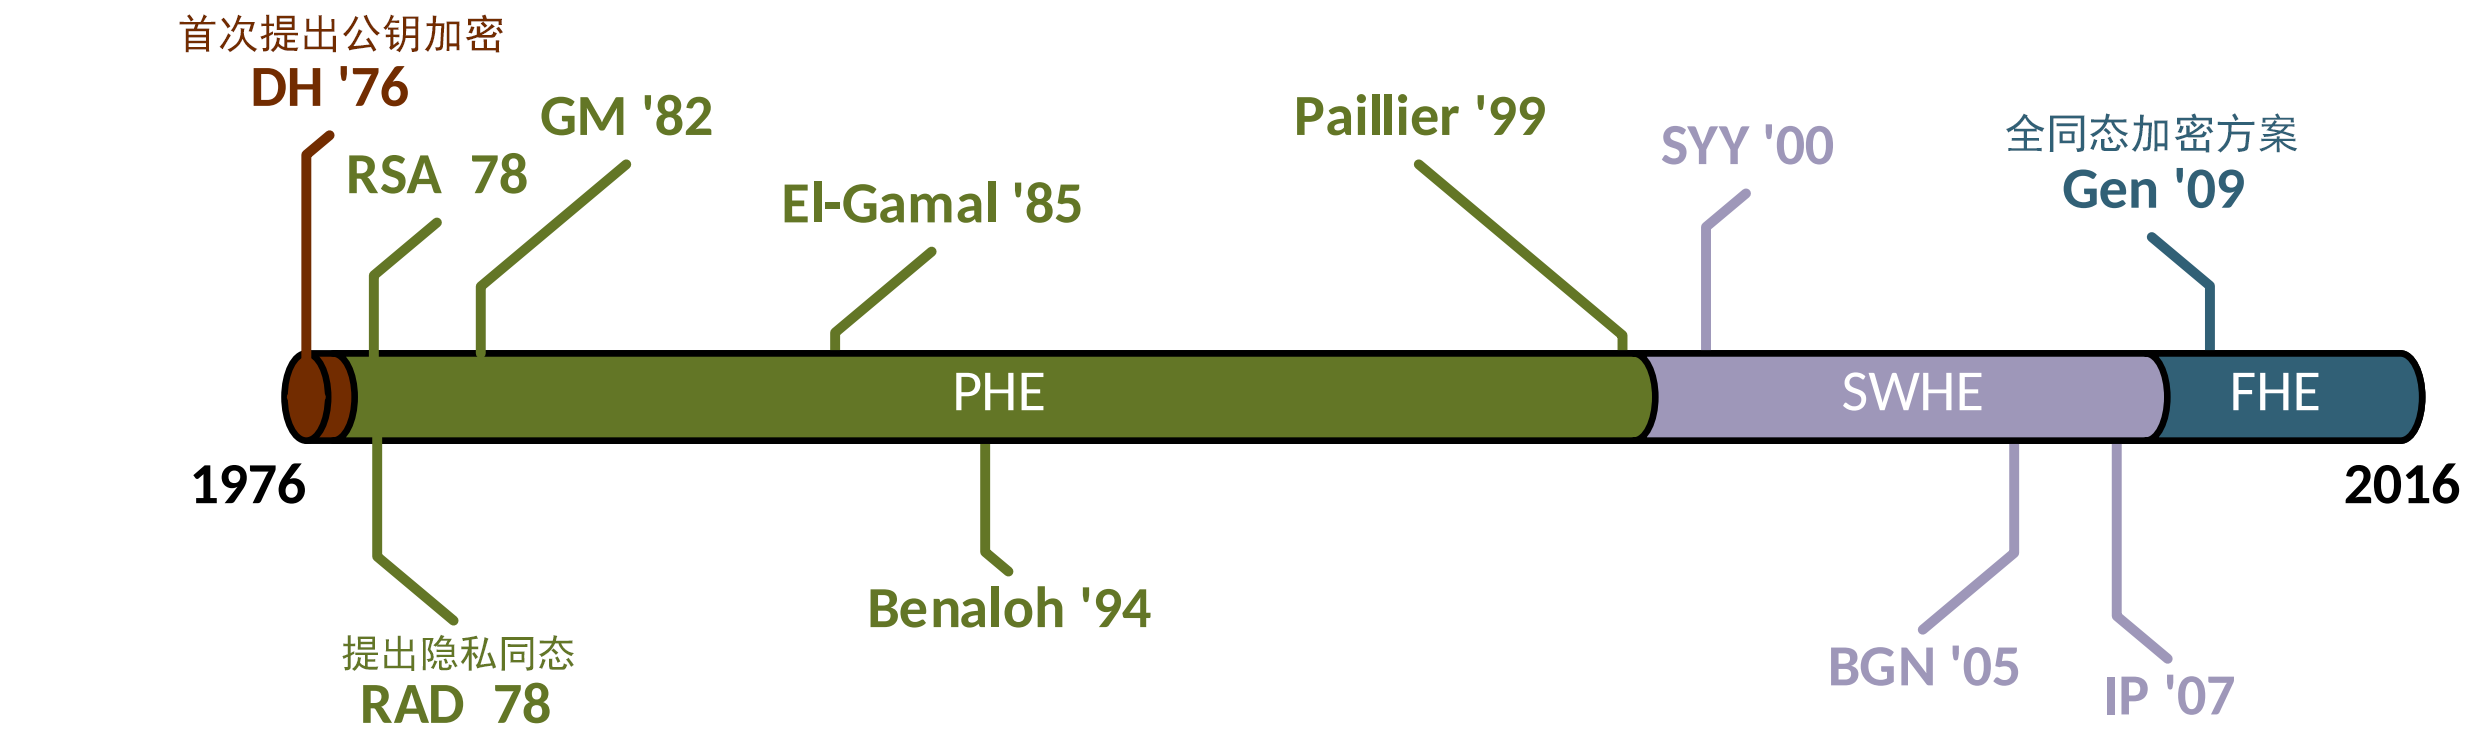
\includegraphics[scale=1.0\linewidth]{img/timeline.png}%width=\line/width
	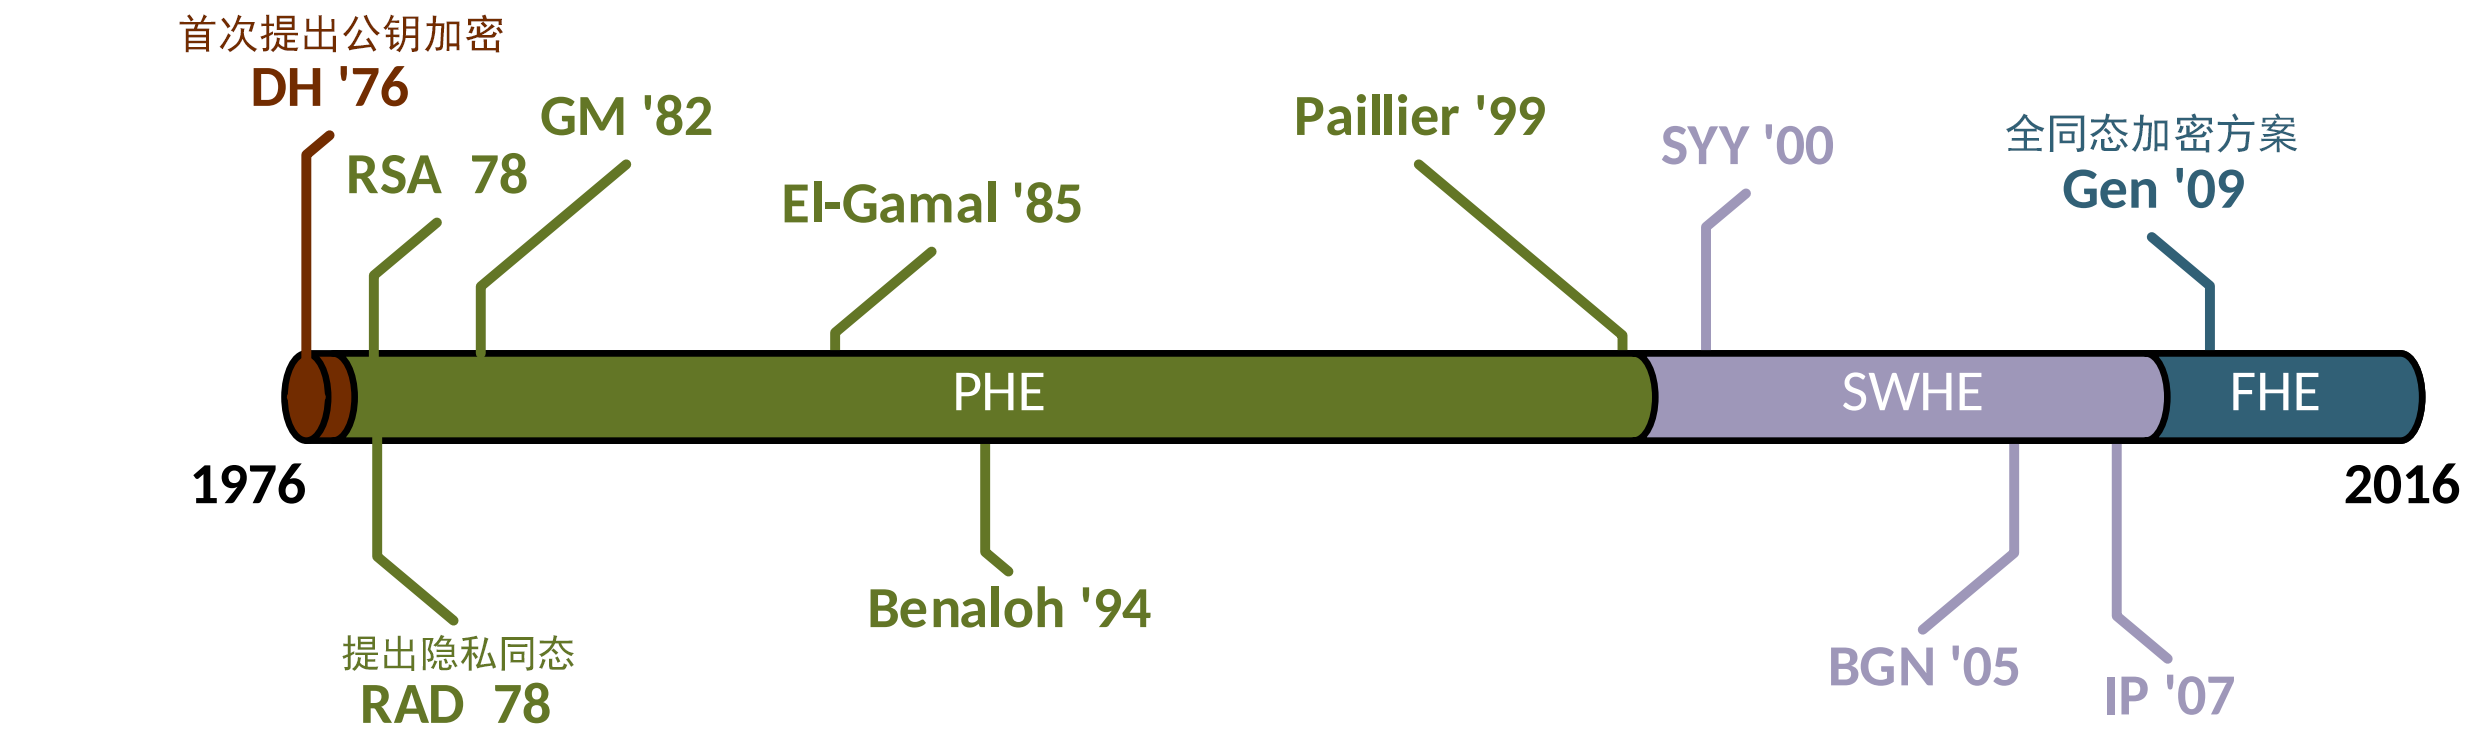
\includegraphics[scale=0.17]{img/timeline.png}
	\caption{同态加密发展时间线}
	\label{timeline}
\end{figure}

和经典的加密方式不同的是,同态加密允许直接在加密数据上进行计算,而不需要访问密钥。计算的结果仍然处于加密状态,并且可以通过密钥解密还原明文结果,目前同态加密相关研究已经取得了诸多成果。
具体定义\cite{acar2018survey}如下:

\begin{definition}
	若一个加密方案支持如下公式,则称为操作$ \star $上的同态
	\begin{equation}
		E\left(m_1\right) \star E\left(m_2\right)=E\left(m_1 \star m_2\right), \quad \forall m_1, m_2 \in M
	\end{equation}

	其中$ E $为加密算法,$ M $为所有可能信息的集合。
\end{definition}

同态加密可以进一步细分为三类,分别是部分同态加密(Partially Homomorphic Encryption,PHE)、类同态加密(Somewhat Homomorphic Encryption,SWHE)以及全同态加密(Fully Homomorphic Encryption,FHE)。三者的区别如下表\ref{s1-table-he}所示:

\begin{table}[htbp]
	\renewcommand{\arraystretch}{1.3}
	\caption{同态加密方案对比}
	\label{s1-table-he}
	\scalebox{0.9}{
	\begin{tabular}{c|c|c|c}
	\hline
	同态加密类型 & 支持的操作类型 & 操作次数 & 常见加密方案                                   \\
	\hline
	PHE          & 加法或乘法     & 无限次   & RSA、Goldwasser-Micali、El-Gamal以及Paillier等 \\
	\hline
	SWHE         & 加法和乘法     & 有限次   & BGN                                            \\
	\hline
	FHE          & 加法和乘法     & 无限次   & GH11                                           \\
	\hline
\end{tabular}	

}


\end{table}

%\begin{compactitem}
%	\item \textbf{部分同态加密:}Partially Homomorphic Encryption(PHE)支持在密文上进行同一类型的操作无数次,该操作为加法或者乘法。常见的加密方案包括RSA、Goldwasser-Micali、El-Gamal以及Pallier等。
%	\item \textbf{类同态加密:}Somewhat Homomorphic Encryption(SWHE)支持对密文进行有限次的任意操作。常见的加密方案有BGN。
%	\item \textbf{完全同态加密:}Fully Homomorphic Encryption(FHE)支持对密文进行无限次任意操作,并且输出结果仍在密文空间内。常见的加密方案有Gentry等人\cite{gentry2011implementing}提出的GH11等。
%\end{compactitem}

同态加密目前已有诸多应用,例如加密搜索,即在同态加密的基础上使搜索引擎不知道用户搜索真正内容的前提下获取搜索结果。
安全求交,也称为隐私集合求交,该技术允许多个参与方在不公开各自数据的前提下,协同查找出交集数据,且不泄露交集数据以外的隐私信息。
多方联合建模能够在不泄露任何隐私的前提下,结合多方数据以提高模型效果,例如医疗机构协同诊断、银行联合反欺诈等等。
同态加密具有诸多优点,在不受信任的环境下(例如云环境或者第三方)数据仍能保证安全和隐私,消除了数据可用性与数据隐私之间的权衡问题,无需为了数据的隐私而放弃任何数据特征,以及能够抵御量子攻击。

同态加密经过数十年的发展,从最初的半同态加密方案到现在提出的全同态加密方案,已经取得了长足进展,能够满足不同应用场景和复杂计算需求,但是由于该加密方案计算开销较大,效率较低,仍然难以广泛应用于实际生产环境中,性能仍有很大的优化空间。

\subsubsection{安全多方计算}
安全多方计算(Secure Multi-Party Computation,SMPC)允许多个参与方之间协同进行安全的计算操作,而不泄露私有数据。每个参与方都只能看到自己输入的内容,无法获知其他参与方的输入。安全多方计算与外包计算的不同之处在于,协议的执行者同时也是数据的拥有者\cite{2018A}。

安全多方计算已经有诸多隐私保护应用,例如姚式百万富翁问题\cite{1982Protocols}、安全拍卖、投票、安全机器学习\cite{2017Oblivious}等。其中主流技术包括不经意传输(Oblivious Transfer,OT)、混淆电路(Garbled Circuits,GC)以及秘密共享(Secret Sharing,SS)。具体介绍如下:
\begin{compactitem}
	\item \textbf{不经意传输:}是安全计算协议中一个非常重要的基础模块。标准的1-out-of-2 OT的定义涉及两方,发送方$ S $持有两个秘密$ x_0,x_1$,接收方$ R $持有一个选择比特$ b\in\{0,1\} $。OT允许$ R $获得$ x_b $,同时不知道$ x_{1-b} $的内容,$ S $无法得知$ R $获得了什么内容。针对OT计算成本较高等特点,已有多种研究提出了改进方案。
	\item \textbf{混淆电路:}是最广为人知的多方计算技术。有许多协议和方案都是基于混淆电路设计,适用于各种计算操作,包括简单的加法乘法,复杂的比较排序等。但是混淆电路计算成本相对较高,需要每个参与方进行大量通信,因此通信复杂度较高,同时设计协议比较复杂。目前许多研究工作从降低通信开销\cite{goyal2008efficient}、减少电路执行时间\cite{malkhi2004fairplay}以及减少电路门数\cite{pinkas2009secure}来优化电路的使用。
	\item \textbf{秘密共享:}是一种将原始信息划分为$n$个部分,分配给不同的参与方,只有满足$t$个参与方合作才能恢复出原始秘密信息的重要密码学技术。基于秘密共享的复杂安全协议,通常需要参与方之间进行频繁通信,带来较大通信开销,限制了方案的可扩展性。为了能够扩展到多个参与方的的场景,一些研究工作借助大数据计算框架进行并行计算以提升效率减少通信开销。
\end{compactitem}

自安全多方计算被提出后,已经取得了长足进展,部署多方计算的开销下降了3-9个数量级。但是除了上述进展,在多方计算被大规模用于隐私保护应用之前还需要解决几个主要挑战。
\begin{compactitem}
	\item \textbf{开销:}多方计算协议的开销跨度非常大,从几乎可忽略到不能接受,主要取决于设定的威胁模型以及实现的功能。通常数据中心内部的带宽费用非常低,但是实际情况下,通常会将计算外包给不同的云服务提供商以防止数据被窃取,因此带宽开销不可忽视。
	\item \textbf{安全与效率权衡:}目前有一些研究选择在安全和效率之间折中。通过在核心协议中放弃一些强安全性保证来获取效率的极大提升。但是牺牲安全性保证会带来多大的数据安全问题仍有待研究。
\end{compactitem}

在表格\ref{s1-table-pet}中,总结归纳了几种不同的隐私保护技术的特点。随着研究的深入,越来越多学者提出了结合多种不同隐私保护技术的方案,扬长避短,并取得了不错的成果\cite{2015ABY,jagannathan2005privacy,su2007privacy,bozdemir2021privacy}。

\begin{table}[htbp]
	\centering
	\renewcommand{\arraystretch}{1.3}
	\caption{隐私保护技术对比}
	\label{s1-table-pet}
	\scalebox{0.95}{
		\begin{tabularx}{\textwidth}{c|X|X|X|X}
			\hline  % 在表格最上方绘制横线
			技术名称     & \multicolumn{1}{c|}{特点}  & \multicolumn{1}{c|}{优点}  & \multicolumn{1}{c|}{缺点}  & \multicolumn{1}{c}{应用场景}       \\%&SKD
			\hline % 在表格最下方绘制横线
			差分隐私     & 添加噪声扰动数据           & 隐私性好,效率高           & 影响数据质量,可用性不高   & 算力较弱,对数据精度要求较低的场景 \\
			\hline
			同态加密     & 允许在密文上进行计算       & 保护数据安全               & 计算开销大,复杂计算效率低 & 算力较强,隐私保护要求高           \\
			\hline
			安全多方计算 & 数据持有方协同进行隐私计算 & 保护数据安全,计算结果准确 & 通信开销大,效率较低       & 分布式场景                         \\
			\hline
		\end{tabularx}
	}
\end{table}

\subsection{隐私保护聚类方案设计目标}
%目标是准确性、安全性、高效性
云环境下设计隐私保护聚类系统要实现的目标主要有以下三点:
\begin{compactitem}
	\item \textbf{准确性:}用户使用秘密共享、同态加密等技术处理数据后上传到云平台进行聚类,虽然保障了数据的隐私安全,但是对聚类方案的设计带来了挑战。准确性要求在密文的基础上设计系列协议实现聚类的功能,最后得到和明文一致的准确结果。
	\item \textbf{安全性:}输入数据、计算中间结果、输出结果均与数据安全息息相关。一旦某一个环节出问题,都可能会导致隐私被泄露,带来巨大损失。因此隐私保护聚类方案要保护数据以及所有相关结果的安全性。外包计算场景中,执行协议的云服务器无法窥视数据。联合数据进行训练获取结果的每个用户无法获取其他用户的私密数据。
	\item \textbf{高效性:}随着互联网快速发展,用于聚类的数据量日益增加。在明文上进行聚类的耗时和开销已不可忽视,隐私保护方案通常计算和通信更加复杂,因此会进一步降低效率。除了要设计云平台可以高效执行的隐私保护方案,还要照顾到资源有限的用户,尽量降低用户的计算通信开销。
\end{compactitem}

上述三个目标中,安全性与高效性通常难以兼顾,通常需要设计复杂的计算协议来实现完全安全的方案。一些隐私保护工具会损失数据的准确性,但是带来效率的提升,例如差分隐私技术。在设计方案时需要综合考虑,结合应用场景和实际需求,在三者之间做出取舍,达到平衡。
\section{研究内容和创新点}
云环境下的隐私保护聚类系统,需要兼顾效率与安全。本文针对当前研究中存在的数据泄露、聚类效率低等问题,面向具体的应用场景,基于聚类算法,隐私保护技术构建方案。
本文主要研究内容以及创新点如下:
\subsection{隐私保护外包K-means聚类技术研究}
K-means是机器学习算法中最为常见和流行的一种无监督的聚类算法,常用于数据挖掘分析和特征提取。因其包含的计算简单,便于实现,基于K-means的隐私保护聚类方案研究较多,种类丰富。
然而现有的隐私保护K-means研究中,通常难以兼顾效率与安全,以近几年的前沿研究为例,高效的方案泄露了数据分布\cite{wu2020secure},完全安全的方案则效率过低\cite{jaschke2019unsupervised}。本文在论文\cite{kanungo2002efficient}的基础上,研究了一种利用Kd-tree数据结构提升效率同时保障数据安全的隐私保护外包K-means聚类方案。

在本文的方案中,用户首先在本地基于明文数据构建Kd-tree,通过秘密共享加密数据结构后分别上传至双云服务器,而后云服务器协同执行一系列安全协议,最终获得密文聚类结果。方案的创新点主要包括:(1)基于秘密共享技术和百万富翁协议\cite{rathee2020cryptflow2}构建了一系列安全计算协议,使得云平台可以在密文上完成比较、计算欧式距离、求解极值等运算;(2)与传统K-means算法不同,本文利用Kd-tree数据结构进行计算加速,提出一种全新的隐私保护方案;(3)与现有工作对比,本文的计算与通信开销均较小。

\subsection{隐私保护DBSCAN相关技术研究}
K-means聚类过程简单,因此相关的隐私保护方案研究也非常丰富,但是K-means对数据集以及参数初始化有较高要求,需要人工评估簇个数$ k $,同时在非球形数据集上聚类表现较差,对异常数据比较敏感,适用场景有限。
此外,本文提出的隐私保护外包K-means方案的应用场景为某一个用户持有所有原始数据,不支持多用户共同上传数据训练。
为了解决上述问题,本文基于另一种聚类算法,即DBSCAN,展开研究,针对不同的应用场景和实际需求提出了系列隐私保护DBSCAN方案。DBSCAN算法具有诸多优点,应用场景广泛,包含计算比较简单,对该算法进行隐私保护实现具有较大现实意义。

\subsubsection{隐私保护DBSCAN方案}
\label{fanganyi}
在传统明文DBSCAN方案\cite{1996A}的基础上,已有诸多隐私保护方案的研究\cite{2006Privacy,2021Privacy},但是方案大多效率较低且开销较大,同时没有详细的实验验证和分析。本文结合密度聚类算法的特点对聚类过程进行重新设计,构建了一个高效的隐私保护DBSCAN方案。

协同聚类的用户各自将数据进行秘密共享后,分别发送给不共谋的双云服务器,两个云平台协同运行安全协议,并将计算结果返回给用户。用户恢复明文后,运行简单的还原算法来获取最终的聚类结果。本文提出的隐私保护DBSCAN方案的创新点主要有:(1)提出一种全新的隐私保护DBSCAN的实现方式,构建临时簇来降低计算轮次,将部分简单的结果还原工作移交给用户提升效率;(2)允许多个独立的参与方上传数据协同聚类,在不知道彼此数据的前提下获取最终聚类结果;(3)极大程度上提升了效率,耗时减少近100倍。
\subsubsection{改进的隐私保护DBSCAN方案}
明文DBSCAN方案存在聚类结果不稳定的问题,若数据同时满足被划分到多个簇的条件,则最终的划分结果取决于数据遍历的顺序,打乱顺序后再次排序可能得到不同的结果。因此本文在论文\cite{tran2013revised}的基础上,提出了一种改进的隐私保护DBSCAN方案。

方案的实现流程可以分为初始化,聚类以及还原结果三步。主要的创新点有:(1)针对结果稳定性问题首次提出隐私保护方案;(2)在优化聚类效果的基础上,效率远高于目前的前沿方案\cite{bozdemir2021privacy},耗时缩短近20倍。

\subsubsection{基于DBSCAN的隐私保护层次聚类}
DBSCAN聚类的效果受到关键参数的影响,而参数的设置需要分析数据分布特点,在多用户各自持有数据的场景下难以找到合适的方法确定参数值。同时,对于包含不同密度的数据集,传统DBSCAN方案难以获取合理的聚类结果,可能出现较小簇或者单个点的情况。为了解决上述问题,本文基于论文\cite{latifi2021dbhc}的思想,借助$ k $线图和$ k $近邻算法,提出了一个基于DBSCAN的隐私保护层次聚类方案。

方案分为获取eps值、计算初始簇、合并初始簇还原结果三个步骤。用户上传加密数据到双云服务器后,云平台通过执行系列给定的安全协议,获取最终结果并发送给用户。本方案的创新点主要有:(1)基于秘密共享设计了安全排序协议;(2)无需人工给出关键参数,减少用户计算开销;(3)适应包含不同密度数据的数据集,应用更加广泛。

\section{论文组织结构}

本文主要分为5个章节,组织结构如图\ref{lunwenjiegou}所示。

第一章是绪论,首先介绍了云计算和聚类的基本概念,通过剖析云环境下聚类的发展应用,引出了研究云环境下聚类所面临的数据安全和效率问题的意义。然后概述了设计隐私保护聚类方案可能利用的密码学技术及其优缺点,并给出了隐私保护聚类系统的设计目标。最后,简要介绍了本文的主要工作与贡献。

第二章是相关研究综述。本章调研了近年来隐私保护K-means方案以及隐私保护DBSCAN方案的相关研究,通过横向以及纵向对比,总结归纳了不同方案的优缺点。

第三章是隐私保护外包K-means聚类方案。现有的隐私保护K-means聚类方案大多无法兼顾效率与数据安全。为了在保证安全的基础上提升效率,减少用户的计算和通信开销,本文借助Kd-tree数据结构,基于秘密共享设计了一系列安全协议,实现了安全高效的聚类方案。通过安全性分析、理论分析以及全面的实验评估,验证了方案的有效性和安全性,以及高效率。

第四章是隐私保护密度聚类方法研究。针对K-means聚类中存在的各种问题,提出了系列基于DBSCAN的隐私保护聚类方案,分别解决了K-means不适合非凸样本簇、传统DBSCAN聚类结果不稳定以及传统DBSCAN不适合多密度数据集的问题。通过系列分析,验证了方案的正确性、安全性和高效性。

第五章是总结与展望。本章首先总结了本文的研究工作,然后基于此对未来工作进行了展望。

\begin{figure}[htbp]
	\centering
	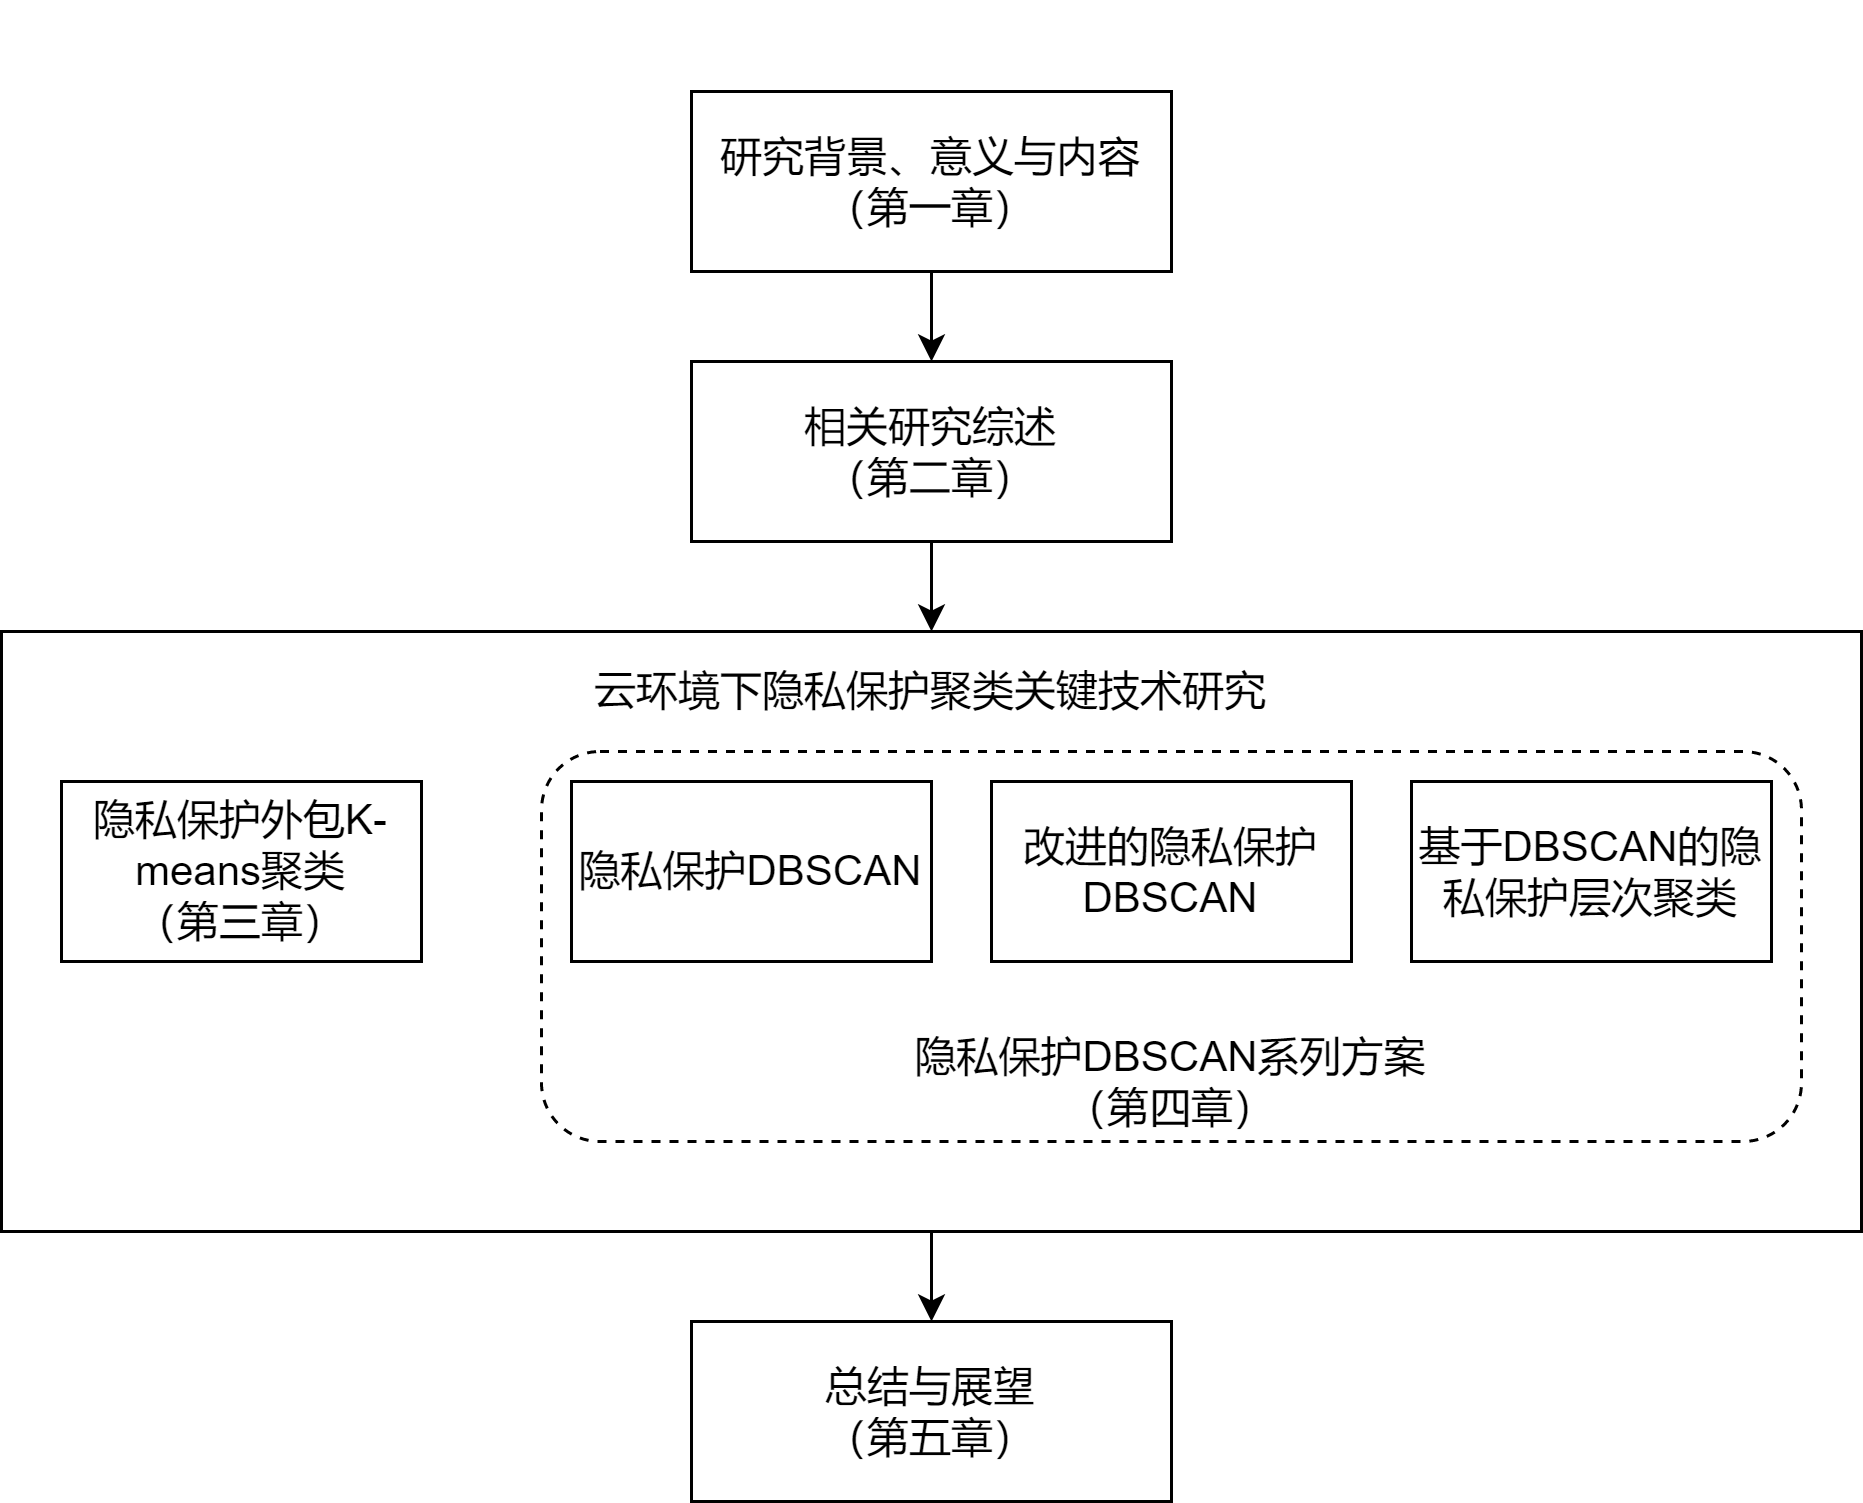
\includegraphics[scale=0.9]{img/dd.png}%width=\linewidth
	\caption{论文组织结构}
	\label{lunwenjiegou}
\end{figure}
\chapter{相关研究综述}


\section{相关理论综述}


\section{国内外研究现状}


%%% Local Variables:
%%% mode: latex
%%% TeX-master: "../main"
%%% End:

\begin{ack}
论文进入尾声,我的研究生涯也将结束。从为科大而准备考研起,我就一直过着充实丰富又踏实的生活,在这个过程中,我遇到了厉害又负责的老师,遇到了友好又可爱的朋友们,遇到了耐心又有趣的师门同学,也遇到了我的另一半,这一段人生旅程是我一生的美好回忆与力量源泉。

感谢我的导师付绍静老师,老师在生活和学习上都给予我们充分的关心和照拂,研一时常询问我们是否在学习生活上有困难,在和老师聊天的过程中,我也慢慢找到了努力的方向。老师言传身教,总是在清晨和深夜看到老师忙碌的身影,我深受鼓舞。老师积极的生活态度,严谨的治学态度以及如沐春风的待人态度,是我永远的学习方向。

感谢柳林老师和罗玉川老师对我的指导。罗玉川老师总是在组会上提出针对性的问题,让我发掘知识盲点。柳老师指导我找到了研究方向,告诉我如何看论文,写论文。老师总能在我研究卡壳的时候,给我提供新的思考角度和突破方向。感谢老师不辞辛苦,耐心指教,时时敦促,我才能一直投入学习不敢松懈。

感谢师门中的各位同学,师兄刘开放、张富成和杨璐铭,师姐范书珲、黄雪伦和冯丹,同级好友陈丽杰、赵侠男、王寅秋和杨旭,师弟师妹黄欣怡、杨钰婷和刘琨鹏等人。和大家一起留下了很多难忘的回忆,师兄们常和我们聊天分享各种经验,雪伦师姐常在我沮丧时悉心开导我,尤记一起在301实验室学习到深夜,丽杰、侠男、寅秋和小杨都是非常有趣善良的人,我们一起努力奋斗,感谢他们充实丰富了我的读研生活,小黄师妹认真踏实乐于分享。与罗淞巍相遇于科大,相识于师门,相熟于网安课程,相恋于初春,相守至今,我们一起阅读健身学习工作,感谢一路的陪伴和支持,今后也要一起奋进美好新生活。

感谢我的家人和朋友们,父母给我提供了莫大的支持,让我没有后顾之忧,母亲一直以来都是我最坚强的后盾,没有她,就没有我的今天。她乐观的态度,坚强的性格和真诚的处世之道,是我一生最宝贵的财富。父母文化水平有限,一生辛勤工作不求回报,只为拖举着我去看更大的世界。感谢相识逾十年的好友小姚小佳,我们一起分享生活分享快乐。感谢大学室友冬倩萧萧舒妤,相离未相忘,你们的陪伴让我的生活趣味良多,感谢我的室友朱姝和许诗瑶,小朱同学打游戏总是给我带来很多快乐,小许同学认真的性格上进的态度让我受益良多。

凡是过往,皆为序章。感恩相遇,希望今后我们都心有所想,事有所成,在各自的人生道路上发光发热。
\end{ack}


%</thesis>
%    \end{macrocode}
%
% 在\LaTeX{}下管理参考文献将极其方便,建议使用Jabref生成条目,
% 用\verb|\cite|(其中\verb|upcite|是上标索引)索引即可。
% \verb|refs.bib|是你的参考文献名。
%    \begin{macrocode}
%<*thesis>
\cleardoublepage
\phantomsection
\addcontentsline{toc}{chapter}{参考文献}
\ifisbiber
{\hyphenpenalty=500 %
\tolerance=9900 %
\renewcommand{\baselinestretch}{1.35}
\printbibliography[heading=bibliography, title=参考文献]

}
\else
\bibliographystyle{bstutf8}
\bibliography{ref/refs}
\fi

\begin{resume}
\ifreview

\ifismaster
该论文作者在学期间取得的阶段性成果(学术论文等)已满足我校硕士学位评阅相关要求。为避免阶段性成果信息对专家评价学位论文本身造成干扰,特将论文作者的阶段性成果信息隐去。
\else
该论文作者在学期间取得的阶段性成果(学术论文等)已满足我校博士学位评阅相关要求。为避免阶段性成果信息对专家评价学位论文本身造成干扰,特将论文作者的阶段性成果信息隐去。
\fi

\else

\ifisresumebib
该论文作者在学期间取得的阶段性成果(学术论文等)已满足我校硕士学位评阅相关要求。为避免阶段性成果信息对专家评价学位论文本身造成干扰,特将论文作者的阶段性成果信息隐去。
%	\begin{refsection}[ref/resume.bib]
%	\settoggle{bbx:gbtype}{false}%局部设置不输出文献类型和载体标识符
%	\settoggle{bbx:gbannote}{true}%局部设置输出注释信息
%	\setcounter{gbnamefmtcase}{1}%局部设置作者的格式为familyahead格式
%	\nocite{ref-1-1-Yang,ref-2-1-杨轶,ref-3-1-杨轶,ref-4-1-Yang,ref-5-1-Wu,ref-6-1-贾泽,ref-7-1-伍晓明}
%	
%	\setlength{\biblabelsep}{12pt}
%	\printbibliography[env=resumebib,heading=subbibliography,title={发表的学术论文}] % 发表的和录用的合在一起
%
%	\end{refsection}


%	\begin{refsection}[ref/resume.bib]
%	\settoggle{bbx:gbtype}{false}%局部设置不输出文献类型和载体标识符
%	\settoggle{bbx:gbannote}{true}%局部设置输出注释信息
%	\setcounter{gbnamefmtcase}{1}%局部设置作者的格式为familyahead格式
%	\nocite{ref-8-1-任天令,ref-9-1-Ren}%
%	
%	\setlength{\biblabelsep}{12pt}
%	\printbibliography[env=resumebib,heading=subbibliography,title={研究成果}]
%
%	\end{refsection}

\else

%  \section*{发表的学术论文} % 发表的和录用的合在一起
%
%  \begin{enumerate}[label={[\arabic*]}]
%
%  \end{enumerate}
%
%  \section*{研究成果} % 有就写,没有就删除
%  \begin{enumerate}[label=\textbf{[\arabic*]}]
%  \addtolength{\itemsep}{-.36\baselineskip}%
%  \item 任天令, 杨轶, 朱一平, 等. 硅基铁电微声学传感器畴极化区域控制和电极连接的
%    方法: 中国, CN1602118A. (中国专利公开号.)
%  \item Ren T L, Yang Y, Zhu Y P, et al. Piezoelectric micro acoustic sensor
%    based on ferroelectric materials: USA, No.11/215, 102. (美国发明专利申请号.)
%  \end{enumerate}
\fi
\fi
\end{resume}

%</thesis>
%    \end{macrocode}
%
%<thesis>% 最后,需要的话还要生成附录,全文随之结束。
%    \begin{macrocode}
%<*thesis>
\appendix
\backmatter
% TeX
\chapter{模板提供的希腊字母命令列表}

大写希腊字母:
\begin{table}[htbp]
\centering
\begin{tabular}{llll}
\toprule
$\Gamma$~\verb|\Gamma| & $\Lambda$~\verb|\Lambda| & $\Sigma$~\verb|\Sigma| & $\Psi$~\verb|\Psi| \\
$\Delta$~\verb|\Delta| & $\Xi$~\verb|\Xi| & $\Upsilon$~\verb|\Upsilon| & $\Omega$~\verb|\Omega| \\
$\Theta$~\verb|\Theta| & $\Pi$~\verb|\Pi| & $\Phi$~\verb|\Phi| & \\
\midrule
$\varGamma$~\verb|\varGamma| & $\varLambda$~\verb|\varLambda| & $\varSigma$~\verb|\varSigma| & $\varPsi$~\verb|\varPsi| \\
$\varDelta$~\verb|\varDelta| & $\varXi$~\verb|\varXi| & $\varUpsilon$~\verb|\varUpsilon| & $\varOmega$~\verb|\varOmega| \\
$\varTheta$~\verb|\varTheta| & $\varPi$~\verb|\varPi| & $\varPhi$~\verb|\varPhi| & \\
\bottomrule
\end{tabular}
\end{table}

小写希腊字母:
\begin{table}[htbp]
\centering
\begin{tabular}{llll}
\toprule
$\alpha$~\verb|\alpha| & $\theta$~\verb|\theta| & $o$~\verb|o| & $\tau$~\verb|\tau| \\ 
$\beta$~\verb|\beta| & $\vartheta$~\verb|\vartheta| & $\pi$~\verb|\pi| & $\upsilon$~\verb|\upsilon| \\ 
$\gamma$~\verb|\gamma| & $\iota$~\verb|\iota| & $\varpi$~\verb|\varpi| & $\phi$~\verb|\phi| \\ 
$\delta$~\verb|\delta| & $\kappa$~\verb|\kappa| & $\rho$~\verb|\rho| & $\varphi$~\verb|\varphi| \\ 
$\epsilon$~\verb|\epsilon| & $\lambda$~\verb|\lambda| & $\varrho$~\verb|\varrho| & $\chi$~\verb|\chi| \\ 
$\varepsilon$~\verb|\varepsilon| & $\mu$~\verb|\mu| & $\sigma$~\verb|\sigma| & $\psi$~\verb|\psi| \\ 
$\zeta$~\verb|\zeta| & $\nu$~\verb|\nu| & $\varsigma$~\verb|\varsigma| & $\omega$~\verb|\omega| \\ 
$\eta$~\verb|\eta| & $\xi$~\verb|\xi| & $\varkappa$~\verb|\varkappa| & $\digamma$~\verb|\digamma| \\ 
\midrule
$\upalpha$~\verb|\upalpha| & $\uptheta$~\verb|\uptheta| & $\mathrm{o}$~\verb|\mathrm{o}| & $\uptau$~\verb|\uptau| \\ 
$\upbeta$~\verb|\upbeta| & $\upvartheta$~\verb|\upvartheta| & $\uppi$~\verb|\uppi| & $\upupsilon$~\verb|\upupsilon| \\ 
$\upgamma$~\verb|\upgamma| & $\upiota$~\verb|\upiota| & $\upvarpi$~\verb|\upvarpi| & $\upphi$~\verb|\upphi| \\ 
$\updelta$~\verb|\updelta| & $\upkappa$~\verb|\upkappa| & $\uprho$~\verb|\uprho| & $\upvarphi$~\verb|\upvarphi| \\ 
$\upepsilon$~\verb|\upepsilon| & $\uplambda$~\verb|\uplambda| & $\upvarrho$~\verb|\upvarrho| & $\upchi$~\verb|\upchi| \\ 
$\upvarepsilon$~\verb|\upvarepsilon| & $\upmu$~\verb|\upmu| & $\upsigma$~\verb|\upsigma| & $\uppsi$~\verb|\uppsi| \\ 
$\upzeta$~\verb|\upzeta| & $\upnu$~\verb|\upnu| & $\upvarsigma$~\verb|\upvarsigma| & $\upomega$~\verb|\upomega| \\ 
$\upeta$~\verb|\upeta| & $\upxi$~\verb|\upxi| & & \\ 
\bottomrule
\end{tabular}
\end{table}

希腊字母属于数学符号类别,请用\verb|\bm|命令加粗,其余向量、矩阵可用\verb|\mathbf|。


\end{document}
%</thesis>
%    \end{macrocode}
%
% 当然还有一些收尾工作,校验审阅自不必说。接下来你需要:修改论文中英文日期,
% 生成盲评,生成明(盲)评A3封面。
%
% {\color{blue}Happy \TeX{}ing! 欢迎提各式各样的意见!}
%
% \newpage\relax%
%
% \StopEventually{\PrintChanges}
% \clearpage
%
% \section{实现细节}
% 我们首先介绍文档模板的基本信息以及宏包和配置,
% 然后依照国防科技大学论文模板的书写规范一节一节的介绍实现步骤。
%
% \changes{v1.2}{2009/09/28}{添加了A3封面制作}
%
% \subsection{基本信息}
%    \begin{macrocode}
%<cls>\NeedsTeXFormat{LaTeX2e}[1999/12/01]
%<cls>\ProvidesClass{nudtpaper}
%<cfg>\ProvidesFile{nudtpaper.cfg}
%<cls|cfg>[2020/07/01 v2.8 NUDT paper template]
%    \end{macrocode}
%
% \subsection{宏包配置}
%
%<*cls>
%
%\changes{v0.99}{2009/08/17}{add package options}
% 当前的宏包选项在之前已经介绍了,下面是实现步骤,就是几个\verb|if|。
%\changes{v1.6}{2009/12/01}{添加单独的单双面控制}
%\changes{v2.0}{2010/11/09}{添加盲评控制}
%\changes{v2.8}{2020/07/01}{添加文献生成选项、添加成果论文生成选项}
%    \begin{macrocode}
\newif\ifismaster\ismastertrue
\DeclareOption{master}{\ismastertrue}
\DeclareOption{doctor}{\ismasterfalse}
\newif\ifisanon\isanonfalse
\DeclareOption{anon}{\isanontrue}
\newif\ifistwoside\istwosidefalse
\DeclareOption{twoside}{\istwosidetrue}
\DeclareOption*{\PackageWarning{nudtpaper}{Unknown Option '\CurrentOption'}}
% handle fonts
\newif\ifisttf\isttffalse
\newif\ifisotf\isotffalse
\newif\ifisfz\isfzfalse
\newif\ifisfandol\isfandolfalse
\DeclareOption{ttf}{\isttftrue}
\DeclareOption{otf}{\isotftrue}
\DeclareOption{fz}{\isfztrue}
\DeclareOption{fandol}{\isfandoltrue}
%<cls>%add biber option
%<cls>%if biber is set, use biblatex to generate bibliography
\newif\ifisbiber\isbiberfalse
\DeclareOption{biber}{\isbibertrue}
%<cls>%add resumebib option
%<cls>%if resumebib is set, use biblatex to generate resume
\newif\ifisresumebib\isresumebibfalse
\DeclareOption{resumebib}{\isresumebibtrue}
\ProcessOptions\relax
%    \end{macrocode}
%
% 首先调用在文档类书写中需要的过程控制语句,在计算一些\verb|length|时要用到
%    \begin{macrocode}
\RequirePackage{ifthen,calc}
%    \end{macrocode}
%
% 接着我们导入文本类,该模板基于标准的书籍模板book,其默认格式为单面打印。
% 博士论文如需双面打印,必须指定\verb|twoside|选项。双开的含义是章节总是
% 起在右手边,左手空白页为完全的空白页,不包含页眉页脚。
%
% \changes{v1.6}{2009/12/01}{修改开关选项}
%
%    \begin{macrocode}
\ifistwoside
  \LoadClass[a4paper,12pt,openright,twoside]{book}
\else
  \LoadClass[a4paper,12pt,openany]{book}
\fi
%    \end{macrocode}
%
% 我们直接用\textsf{geometry}宏包进行页面边距的设定,调用titlesec设定标题以及页眉页脚,
% 用\textsf{titletoc}设定目录格式。需要改动的可以参考这三个宏包的说明文档。
%
%    \begin{macrocode}
\RequirePackage[includeheadfoot]{geometry}
\RequirePackage[center,pagestyles]{titlesec}
\RequirePackage{titletoc}
%    \end{macrocode}
%
% 文档中另外重要的两个部分是表格和图片。
% 首先来看图片:\textsf{graphicx}宏包是必不可少的,
% 并排图形。\textsf{subfigure} 已经不再推荐,用新的 \textsf{subfig}。
% 加入 \verb|config| 选项
% 以便兼容 \textsf{subfigure} 的命令。浮动图形和表格标题样式。\textsf{caption2} 已经不
% 推荐使用,采用新的 \textsf{caption}。它会自动被 \textsf{subfig} 装载进来。所以可以在
% 后面使用 \textbf{captionsetup} 命令,宏包\textsf{float}的作用是可以用H命令,
% 将浮动对象强制放在这里(副作用是版面可能不好):
%
%    \begin{macrocode}
\RequirePackage{graphicx}
\RequirePackage[config]{subfig}
\RequirePackage{float}
%    \end{macrocode}
%
% 再来看表格:我们采用\textsf{longtable}来处理长的表格,还需要\textsf{array}包;
% 标准的论文需要表格为三线表,这里引用\textsf{booktabs}宏包来处理,
% 这样,我们就可以简单的使用\verb|\toprule|,\verb|\midrule|,\verb|bottomrulle|
% 这样的命令;
% 为了在表格中支持跨行,需要引入\textsf{multirow}包,\textsf{tabularx}的作用是为了使用
% 固定宽度的表格,\textsf{slashbox}可以让我们在表格中使用反斜线:
%    \begin{macrocode}
\RequirePackage{array}
\RequirePackage{longtable}
\RequirePackage{booktabs}
\RequirePackage{multirow}
\RequirePackage{tabularx}
\RequirePackage{slashbox}
%    \end{macrocode}
% 表格和图片的例子可以搜索C\TeX{}论坛或者看示例文件。
%
% 引入\textsf{paralist}来达到比较好看的列表环境
%    \begin{macrocode}
\RequirePackage[neverdecrease]{paralist}
\RequirePackage{enumitem}
%    \end{macrocode}
%
% 文档中还需要一定的色彩控制和字体控制
%    \begin{macrocode}
\RequirePackage{xcolor}
%    \end{macrocode}
%
% 为了排出漂亮的数学公式,\textsf{amsmath}包是必不可少的,
% 需要注意的是,新版本的论文模不再使用\textsf{txfonts}宏包,
% 为了支持希腊正体字母,需要调用\verb|upgreek.sty|,使用方法是\verb|\up<greek>|。
% 注意到这个宏包前面加上了\verb|Symbolsmallscale|选项,这是为了调整希腊字母的大小而设定的。
% 如果用户不满意这个宏包的积分号
% 等符号,倾向与使用传统的\LaTeX{}风格的数学符号,那么可以使用
% \textsf{mathptmx}宏包,但要把\verb|upgreek|的选项改为\verb|Symbol|,要不然
% 正体希腊字母要显得比正常字符小一点哦。
% 而大写斜体希腊字母(变量)可以通过\textsf{amsmath}的\verb|\var<Greek>|得到。
% 对于希腊字母的加粗使用\verb|bm|宏包,而一般变量的加粗那就使用\verb|\mathbf|吧!
% \changes{v2.0}{2010/11/09}{去掉fontspec,传递no-math到xeCJK,加入bm宏包}
% \changes{v2.2}{2011/07/16}{去掉txfonts宏包,使用lm字体,添加svgreek.sty}
% \changes{v2.2}{2011/07/16}{修改,仍旧使用upgreek, mathptmx, bm组合}
% \changes{v2.2}{2011/09/25}{修改,使用upgreek, txfonts, bm组合}
% \changes{v2.2}{2012/11/28}{给用户提供额外的选项,还是mtpro比较漂亮}
% \changes{v2.3}{2013/12/27}{调整数学字体,加入mtpro使用说明,并且仿照IEEE模板,修改displaypenalty}
% \changes{v2.5}{2015/05/11}{去掉txfonts,用默认数学字体}
%    \begin{macrocode}
\RequirePackage{amsmath,amssymb}
\RequirePackage[Symbolsmallscale]{upgreek}
%\RequirePackage{amsmath}
%\RequirePackage[amsbb,eufrak,compatiblegreek,subscriptcorrection,nofontinfo]{mtpro2}
\interdisplaylinepenalty=2500
\RequirePackage{bm}
\RequirePackage[T1]{fontenc}
\RequirePackage[amsmath,thmmarks,hyperref]{ntheorem}
%    \end{macrocode}
% 需要注意的是,如果用户有\verb|mtpro2|包,还是强烈建议使用这个的,因为数学公式
% 在这个包下显得特别的美观。虽然下载和安装不属于这篇使用说明的范畴,但是,上面的注释部分
% 可以给大家如何使用的一个简单的例子。当你安装好\verb|mtpro2|之后,主要取消注释,并且将
% 上面的三个包注释掉即可。
%
% 本文档类直接采用\XeTeX{}引擎,方便了字体配置以及编译,
% 这里需要调用\textsf{XeCJK}宏包,no--math的作用是不改变先前数学宏包设定的数学字体。
% 同时采用\textsf{indentfirst}宏包管理文字的缩进:
% \changes{v1.8}{2010/10/15}{修改了默认的xeCJK的选项,为了兼容旧的xeCJK版本,normalindentfirst选项暂不使用,而是在后面添加indentfirst包}
% \changes{v2.0}{2010/11/10}{传递no-math给xeCJK里面的fontspec宏包}
% \changes{v2.2}{2011/07/03}{移除CJKtextspace, CJKmathspace, CJKnumber选项}
% \changes{v2.4}{2015/02/09}{移除CJKnumber选项,添加新的CJKnumb宏包。旧版本TexLive无需更改。}
% \changes{v2.6}{2017/05/15}{移除CJKnumb宏包,统一使用zhnumber宏包。推荐使用2016以后的TexLive版本。}
% \changes{v2.8}{2020/07/01}{增加xunicode-addon宏包,设置FreeSerif字体,用于显示文献表中的波浪号。}
%
%    \begin{macrocode}
\RequirePackage[CJKchecksingle,no-math]{xeCJK}
\RequirePackage{zhnumber}
\RequirePackage{indentfirst}
\RequirePackage{xunicode-addon}
\newcommand{\fttilde}{\fontspec{FreeSerif}\selectfont}
%    \end{macrocode}
%
% 另外一个关键部分是文献索引,包括书签以及参考文献的索引,记得\textsf{hyperref}配合
% \XeTeX{}使用时暂不能开启Unicode选项,新的发行版已经移除\textsf{hypernat}包。
% 另外还要注意,你最终的打印版肯定不希望有花花绿绿的链接对吧?
% 那就把下面那行\verb|hyperref|注释掉就行了或者把选项改为\verb|\colorlinks=false|即可。
% \changes{v2.1}{2010/12/29}{移除hypernat包}
% \changes{v2.2}{2011/07/17}{移除hyperref的CJKbookmarks旋向}
% \changes{v2.3}{2013/12/27}{加入色彩版hyperref}
% \changes{v2.5}{2015/05/11}{提示用户在最终打印版时去掉链接颜色}
% \changes{v2.8}{2020/07/01}{增加基于biblatex生成文献的方法}
%    \begin{macrocode}
%code for dealing option: biber
\ifisbiber
\RequirePackage[backend=biber,style=gb7714-2015,gbalign=gb7714-2015,%
gbnamefmt=lowercase,gbpub=false]{biblatex}%
\addbibresource[location=local]{ref/refs.bib}
\setlength{\bibitemsep}{1pt}
\setlength{\bibnamesep}{0ex}
\setlength{\bibinitsep}{0ex}
\setlength{\biblabelsep}{6pt}
\newlength{\refindent}
\setlength{\refindent}{24pt}
\renewcommand{\itemcmd}{%
\setlength{\lengthid}{0cm}%
\setlength{\lengthlw}{\textwidth}%
\addtolength{\lengthlw}{-\lengthid}%
\addvspace{\bibitemsep}%恢复\bibitemsep的作用 %\parshape 2 0em \textwidth \lengthid \lengthlw
\hangindent\lengthid%
\hspace{\refindent}\mkgbnumlabel{\printfield{labelnumber}}%
\hspace{\biblabelsep}}
\DefineBibliographyExtras{english}{\renewcommand*{\bibrangedash}{{\fttilde\textsim}}}%将页码间隔符替换会英文的短横线
%<cls>%比如:~$\sim$\symbol{"FF5E}\symbol{"223C}\symbol{"2053}\symbol{"02DC}\symbol{"02F7}
%<cls>%\textsim \textbacksim \texttildebelow \texttildelow \texttilde
\defbibheading{subbibliography}[\bibname]{%
\section*{#1}}
\DeclareDelimFormat{streditortypes}{\bibopenparen%
  \edef\userfieldabcde{userd}%
  \ifcurrentname{editor}{\edef\userfieldabcde{userc}}{}%
  \ifcurrentname{bookauthor}{\edef\userfieldabcde{userb}}{}%
  \ifcase\value{gbbiblocalcase}%
    \iffieldequalstr{\userfieldabcde}{chinese}{\bibstring{\thefield{editortype}scn}}{}%
    \iffieldequalstr{\userfieldabcde}{korean}{\bibstring{\thefield{editortype}skr}}{}%
    \iffieldequalstr{\userfieldabcde}{japanese}{\bibstring{\thefield{editortype}sjp}}{}%
    \iffieldequalstr{\userfieldabcde}{english}{\bibstring{\thefield{editortype}s}}{}%
    \iffieldequalstr{\userfieldabcde}{french}{\bibstring{\thefield{editortype}s}}{}%
    \iffieldequalstr{\userfieldabcde}{russian}{\bibstring{\thefield{editortype}s}}{}%
  \or%
  \bibstring{\thefield{editortype}scn}%
  \or%
  \bibstring{\thefield{editortype}s}%
  \fi\bibcloseparen}
\DeclareDelimFormat{streditortype}{\bibopenparen%
  \edef\userfieldabcde{userd}%
  \ifcurrentname{editor}{\edef\userfieldabcde{userc}}{}%
  \ifcurrentname{bookauthor}{\edef\userfieldabcde{userb}}{}%
  \ifcase\value{gbbiblocalcase}%
    \iffieldequalstr{\userfieldabcde}{chinese}{\bibstring{\thefield{editortype}cn}}{}%
    \iffieldequalstr{\userfieldabcde}{korean}{\bibstring{\thefield{editortype}kr}}{}%
    \iffieldequalstr{\userfieldabcde}{japanese}{\bibstring{\thefield{editortype}jp}}{}%
    \iffieldequalstr{\userfieldabcde}{english}{\bibstring{\thefield{editortype}}}{}%
    \iffieldequalstr{\userfieldabcde}{french}{\bibstring{\thefield{editortype}}}{}%
    \iffieldequalstr{\userfieldabcde}{russian}{\bibstring{\thefield{editortype}}}{}%
  \or%
  \bibstring{\thefield{editortype}cn}%
  \or%
  \bibstring{\thefield{editortype}}%
  \fi\bibcloseparen}
\renewbibmacro*{in:}{%
 \iftoggle{bbx:gbpunctin}{\printtext{\textbf{//}\allowbreak}}%\addthinspace
                         {\setunit{\adddot\addspace}%
                         \iffieldequalstr{userd}{chinese}%
                         {\printtext{\bibstring{incn}}}%
                         {\printtext{\bibstring{in}}}%
                         }}%\newunit\newblock\intitlepunct
\ifisresumebib
\defbibenvironment{resumebib}%修改对齐环境-调整缩进
  {\list
     {\printtext[labelnumberwidth]{%
        \printfield{labelprefix}%
        \printfield{labelnumber}}}
{\setlength{\labelwidth}{\labelnumberwidth}%
      \setlength{\labelsep}{\biblabelsep}%
      \setlength{\leftmargin}{\bibhang}%
      \addtolength{\leftmargin}{\labelnumberwidth}%
      \setlength{\itemindent}{\bibitemindent}%
      \setlength{\itemsep}{\bibitemsep}%
      \setlength{\parsep}{\bibparsep}}%
      \renewcommand*{\makelabel}[1]{\hss##1}}
  {\endlist}
  {\item}
\fi
\else
\RequirePackage[numbers,sort&compress,square]{natbib}
\let\newcite=\cite
\let\parencite=\newcite
\let\inlinecite=\newcite
\newcommand{\upcite}[1]{\textsuperscript{\newcite{#1}}} % 上标形式引用
\renewcommand{\cite}[1]{\textsuperscript{\newcite{#1}}} % 上标形式引用
\fi
\RequirePackage[colorlinks=true,linkcolor=blue,citecolor=red,pdfborder=0 1 1]{hyperref}
\RequirePackage{datetime}
%\RequirePackage[pdfborder=0 0 1]{hyperref}
%    \end{macrocode}
%</cls>
%
%\subsection{基础配置}
% 本章主要介绍模板中用到的基本的元素和定义,现在包括两部分: 字体,字号和字体命令
%
%\subsubsection{字体定义}
% 我们首先来处理\TeX{}中最令人棘手的字体问题,
% 在使用\textsf{XeCJK}包之后,配置和选择很容易,
% 预先设定好一些字体命令是为了后面方便的更改文本字体的需要。
% 首先我们开启\TeX{}连字符:
%    \begin{macrocode}
%<*cls>
\defaultfontfeatures{Mapping=tex-text}
%</cls>
%    \end{macrocode}
%
% 之后用\textsc{XeCJK}包提供的命令设定字体,用户可以选择使用TTF还是OTF字体,
% Adobe的OpenType字体在排版上更具备优势,文档显示锐利,推荐使用。
% 另外在这一个新版本中,我们推荐用户也可以使用方正的字体,只要使用\verb|FZ|选项即可。
% 中注释掉相关的字体就可以。方正字体的有点是标点符号的位置无需修正,且字体之间配合很好。
% \verb|setcharclass|的作用是纠正xunicode、xeCJK的一些设定:
%
% \changes{v0.99}{2009/08/17}{add options TTF and OTF}
% \changes{v1.9}{2010/10/28}{定义一个cusong字体,使用的是中宋}
% \changes{v2.3}{2013/12/27}{用户可以考虑使用方正字体,加入FZ选项}
% \changes{v2.5}{2015/05/11}{重新更改字体选项的调用方式,现在变成三个ttf、otf、fz}
% \changes{v2.5}{2015/05/11}{这种方式用户可以特别方便的添加自己的字体集}
%
%    \begin{macrocode}
%<*cls>
\xeCJKsetcharclass{"0}{"2E7F}{0}
\xeCJKsetcharclass{"2E80}{"FFFF}{1}

% ZhongYi 中易字体
\newcommand{\installttf}{
    %%%% Windows Thesis Fonts
    \setmainfont{Times New Roman PS Std}
    \setsansfont{Arial}
    \setmonofont{Courier New}
    %%%% Using Office Family Fonts
    \setCJKmainfont[BoldFont={STZhongsong}]{SimSun}
    \setCJKsansfont{SimHei} % Hei
    \setCJKmonofont{FangSong} % Fangsong
    %%%% alias
    \setCJKfamilyfont{song}{SimSun}
    \setCJKfamilyfont{hei}{SimHei}
    \setCJKfamilyfont{fs}{FangSong} % fang-song
    \setCJKfamilyfont{kai}{KaiTi} % Kai
}

% Adobe 字体
\newcommand{\installotf}{
    %%%% Windows Thesis Fonts
    \setmainfont{Times New Roman PS Std}
    \setsansfont{Arial}
    \setmonofont{Courier New}
    %%%% Using Adobe Family Fonts
    \setCJKmainfont[BoldFont={STZhongsong}]{Adobe Song Std}
    \setCJKsansfont{Adobe Heiti Std} % Hei
    \setCJKmonofont{Adobe Fangsong Std} % Fangsong
    %%%% alias
    \setCJKfamilyfont{song}{Adobe Song Std}
    \setCJKfamilyfont{hei}{Adobe Heiti Std}
    \setCJKfamilyfont{fs}{Adobe Fangsong Std} % fang-song
    \setCJKfamilyfont{kai}{Adobe Kaiti Std} % Kai
}

% fz 方正字体 [recommended]
\newcommand{\installfz}{
    %%%% Windows Thesis Fonts
    \setmainfont{Times New Roman PS Std}
    \setsansfont{Arial}
    \setmonofont{Courier New}
    %%%% Using Founder Family Fonts
    \setCJKmainfont[BoldFont={FZYaSong-DB-GBK}]{FZShuSong_GB18030-Z01}
    \setCJKsansfont{FZHei-B01} % Hei
    \setCJKmonofont{FZFangSong-Z02} % fs
    %%%% alias
    \setCJKfamilyfont{song}{FZShuSong_GB18030-Z01}
    \setCJKfamilyfont{hei}{FZHei-B01}
    \setCJKfamilyfont{fs}{FZFangSong-Z02} % fang-song
    \setCJKfamilyfont{kai}{FZKai-Z03} % Kai
}

% fandol [incomplete in 2015]
\newcommand{\installfandol}{
    %%%% Windows Thesis Fonts
    \setmainfont{Times New Roman PS Std}
    \setsansfont{Arial}
    \setmonofont{Courier New}
    %%%% Using Fandol Family Fonts
    \setCJKmainfont{FandolSong}
    \setCJKsansfont{FandolHei} % Hei
    \setCJKmonofont{FandolFang} % fs
    %%%% alias
    \setCJKfamilyfont{song}{FandolSong}
    \setCJKfamilyfont{hei}{FandolHei}
    \setCJKfamilyfont{fs}{FandolFang} % fang-song
    \setCJKfamilyfont{kai}{FandolKai} % Kai
}

\ifisttf
\installttf
\fi

\ifisotf
\installotf
\fi

\ifisfz
\installfz
\fi

\ifisfandol
\installfandol
\fi

%</cls>
%    \end{macrocode}
%
% \changes{v1.6}{2009/12/01}{替换OTF英文字体为标准Windows自带字体}
% \changes{v2.3}{2013/12/27}{添加FZ字体选项}
%
% 选定好字体之后,就是设定字体别名,这样我们就可以在文档的其他部分直接使用较短的命令来
% 指定特定的字体了:
%
%    \begin{macrocode}
%<*cls>
% command alias
\newcommand{\cusong}{\bfseries}
\newcommand{\song}{\CJKfamily{song}}     % 宋体
\newcommand{\fs}{\CJKfamily{fs}}         % 仿宋体
\newcommand{\kai}{\CJKfamily{kai}}       % 楷体
\newcommand{\hei}{\CJKfamily{hei}}       % 黑体
\def\songti{\song}
\def\fangsong{\fs}
\def\kaishu{\kai}
\def\heiti{\hei}
%</cls>
%    \end{macrocode}
%
% \subsubsection{字号定义}
%下面就是定义字号大小,这一部分我们有两个参考,其一是:
%
% \begin{verbatim}
% 参考科学出版社编写的《著译编辑手册》(1994年)
% 七号      5.25pt       1.845mm
% 六号      7.875pt      2.768mm
% 小五      9pt          3.163mm
% 五号      10.5pt       3.69mm
% 小四      12pt         4.2175mm
% 四号      13.75pt      4.83mm
% 三号      15.75pt      5.53mm
% 二号      21pt         7.38mm
% 一号      27.5pt       9.48mm
% 小初      36pt         12.65mm
% 初号      42pt         14.76mm
%
% 这里的 pt 对应的是 1/72.27 inch,也就是 TeX 中的标准 pt
% \end{verbatim}
%
% 另外一个来自WORD中的设定:
% \begin{verbatim}
% 初号 = 42bp = 14.82mm = 42.1575pt
% 小初 = 36bp = 12.70mm = 36.135 pt
% 一号 = 26bp = 9.17mm = 26.0975pt
% 小一 = 24bp = 8.47mm = 24.09pt
% 二号 = 22bp = 7.76mm = 22.0825pt
% 小二 = 18bp = 6.35mm = 18.0675pt
% 三号 = 16bp = 5.64mm = 16.06pt
% 小三 = 15bp = 5.29mm = 15.05625pt
% 四号 = 14bp = 4.94mm = 14.0525pt
% 小四 = 12bp = 4.23mm = 12.045pt
% 五号 = 10.5bp = 3.70mm = 10.59375pt
% 小五 = 9bp = 3.18mm = 9.03375pt
% 六号 = 7.5bp = 2.56mm
% 小六 = 6.5bp = 2.29mm
% 七号 = 5.5bp = 1.94mm
% 八号 = 5bp = 1.76mm
%
% 1bp = 72.27/72 pt
% \end{verbatim}
%
% 我们采用习惯的字号设定方法(也就是WORD中的设定),首先编写字体设置命令:
%
%\begin{macro}{\choosefont}
% 我们可以使用 |\choosefont| 来选择字体, 字体设定这些大多是从清华的模板拷过来的。
%
%    \begin{macrocode}
%<*cls>
\newlength\thu@linespace
\newcommand{\thu@choosefont}[2]{%
    \setlength{\thu@linespace}{#2*\real{#1}}%
    \fontsize{#2}{\thu@linespace}\selectfont}
\def\thu@define@fontsize#1#2{%
    \expandafter\newcommand\csname #1\endcsname[1][\baselinestretch]{%
    \thu@choosefont{##1}{#2}}}
%</cls>
%    \end{macrocode}
%\end{macro}
%
%设定具体的字体大小:
%
%    \begin{macrocode}
%<*cls>
\thu@define@fontsize{chuhao}{42bp}
\thu@define@fontsize{xiaochu}{36bp}
\thu@define@fontsize{yihao}{26bp}
\thu@define@fontsize{xiaoyi}{24bp}
\thu@define@fontsize{erhao}{22bp}
\thu@define@fontsize{xiaoer}{18bp}
\thu@define@fontsize{sanhao}{16bp}
\thu@define@fontsize{xiaosan}{15bp}
\thu@define@fontsize{sihao}{14bp}
\thu@define@fontsize{banxiaosi}{13bp}
\thu@define@fontsize{xiaosi}{12bp}
\thu@define@fontsize{dawu}{11bp}
\thu@define@fontsize{wuhao}{10.5bp}
\thu@define@fontsize{xiaowu}{9bp}
\thu@define@fontsize{liuhao}{7.5bp}
\thu@define@fontsize{xiaoliu}{6.5bp}
\thu@define@fontsize{qihao}{5.5bp}
\thu@define@fontsize{bahao}{5bp}
%</cls>
%    \end{macrocode}
%
%\subsubsection{自定命令}
% 有一些常量,测试,自定义的命令等都放在这里,待到论文逐渐完善之后再做定夺,
% 当然用户自己的命令也可以在此添加,事实上如果natbib传递的是superscript,
% \verb|cite|命令默认就成了上标了。这里不加入这个选项,而是单独编写一个命令:
%
%    \begin{macrocode}
%<*cls>
\newcommand{\china}{中华人民共和国}
\def\nudtpaper{\textsc{Nudt}\textsc{Paper}}
\newcommand{\pozhehao}{\kern0.2em\rule[0.8ex]{1.6em}{0.1ex}\kern0.2em}
\newcommand{\xiaopozhe}{\kern0.2em\rule[0.8ex]{0.6em}{0.1ex}\kern0.2em}
%</cls>
%    \end{macrocode}
% \changes{v2.5}{2015/05/11}{添加了一个xiaopozhe命令,用作中文连词符}
%
%\subsubsection{中文元素}
%
% 默认的页面元素的英文名,诸如Contents为目录,Abstract为摘要等,
% 我们首先将他们一一中文化:
% \changes{v0.992}{2009/08/19}{修改图表编号格式}
% \changes{v1.3}{2009/10/14}{修改图目录和表目录}
% \changes{v2.6}{2017/05/15}{更新zhnumber宏包兼容命令}
% \changes{v2.6}{2017/05/15}{重定义zhnumber宏包中的zhtoday命令}
%
%    \begin{macrocode}
%<*cls>
\renewcommand\contentsname{目\hspace{1em}录}
\renewcommand\listfigurename{图\hspace{1em}目\hspace{1em}录}
\renewcommand\listtablename{表\hspace{1em}目\hspace{1em}录}
\newcommand\listequationname{公式索引}
\newcommand\equationname{公式}
\renewcommand\bibname{参考文献}
\renewcommand\indexname{索引}
\renewcommand\figurename{图}
\renewcommand\tablename{表}
\renewcommand\appendixname{附录}
\def\CJK@today{\zhdigits{\the\year}年\zhnumber{\the\month}月}
\renewcommand\zhtoday{\CJK@today}
\newcommand\entoday{\monthname{}, \the\year}
%</cls>
%    \end{macrocode}
%
% 好,下面就开始按照论文模板要求进行排版!
%
%\subsection{编写要求}
% 学校规定,论文需采用白色纸双面打印。
% 学位论文用A4($210mm\times{}297mm$)标准大小的白纸,
% 在打字或印刷时,要求纸的四周留足空白边缘,以便装订、复制和读者批注。
% 每一面的上方(天头)和下方(地角)分别留边25mm,左侧(订口)
% 和右侧(切口)分别留边30mm,页眉与页脚分别为23mm。
%
% 实现起来很简单,只要调用\textsf{geometry}的版面控制命令即可,
% 方法为先把word模板转化为PDF,
% 用Adobe的裁剪功能查看页边距,进行微调,直到比对正确为止,设定如下:
%
% \changes{v0.991}{2009/08/18}{modify bottom skip}
% \changes{v1.1}{2009/09/26}{修改footskip容限以及bottom的值,为了容下longtab的''下一页''}
% \changes{v1.4}{2009/10/28}{减小页眉skip 1mm,用word叠印}
% \changes{v1.4}{2009/10/30}{增大页眉sep .5mm,用word叠印}
%
%    \begin{macrocode}
%<*cls>
\geometry{top=21mm,bottom=25.5mm,left=30mm,right=30mm}
\geometry{headheight=9mm,headsep=1mm,footskip=9mm}
%</cls>
%    \end{macrocode}
%
%\subsection{页眉页脚}
%
% 我们采用titlesec进行页面配置。
% 页面中的主要元素有Chapter,Section,Subsection等元素的外观,
% 位置,颜色字体等,页面元素还包括页眉页脚。这种方法配置简便,易管理。
% 国防科大的论文需要在页眉处画两根横线,我们通过下面的命令实现:
%
%\begin{macro}{\setheadrule}
% 这个命令属于更改\textsf{titlesec}中的一个画页眉的命令,稍加调整:
% \changes{v0.991}{2009/08/18}{modify headrull, s.t. all geometry match}
% \changes{v1.9}{2010/10/28}{去掉headsep,修改headrule,在sethead后添加raisebox}
%
%    \begin{macrocode}
%<*cls>
\renewcommand\setheadrule[1]{%
  \ifdim#1=\z@
    \let\makeheadrule\@empty
  \else
    \def\makeheadrule{%
    \makebox[0pt][l]{\rule[.2\baselineskip]{\linewidth}{1.5pt}}%
    \rule{\linewidth}{1.5pt}}%
  \fi}
%</cls>
%    \end{macrocode}
%\end{macro}
%
% 由于Chapter第一页默认是\verb|plain|页面格式,
% 章节的其余部分是在Matter中设定的页面格式,为了简单起见,
% 我们就直接更改\verb|plain|页面设置,
% 要求为5号宋体居中放置,画页眉页脚,页脚为1磅黑线
%
% \changes{v0.992}{2009/08/20}{renewpagestyle里面前导的空格可能导致clearpage生成新的一页,将空格去掉}
% \changes{v0.993}{2009/08/26}{修改标题,博士硕士对应不同的页眉}
%
%    \begin{macrocode}
%<*cls>
\renewpagestyle{plain}{
\sethead{}{\raisebox{.65\baselineskip}{\songti \wuhao \ifisanon{~}\else{国防科技大学研究生院\@optionpaperclass{}学位论文}\fi}}{}%
\setfoot{}{{\songti \wuhao 第~\thepage~页}}{}%
\headrule%
\footrule%
}
\setfootrule{1bp}
%</cls>
%    \end{macrocode}
%
%\subsection{编写格式}
%
% 当页面设置好之后,就是在论文的不同部分分别调用,一般来说论文类的书籍
% 分为三个matter,为前言区(前置部分),正文区(主体),后文区(附录),
% 在国防科大论文书写要求中,
% 需要将摘要单独进行页码编号,其编号为小写罗马字母,为此,
% 可以将摘要单独设定为一个matter,
% 名叫就叫做MidMatter,称作摘要区。每个Matter我们都一一介绍。
%
% 首先看前置部分,主要包括封面,目录,摘要等,实现为:
%
%    \begin{macrocode}
%<*cls>
\renewcommand\frontmatter{%
    \if@openright\cleardoublepage\else\clearpage\fi
    \@mainmatterfalse
    \pagenumbering{Roman}
    \pagestyle{plain}}
\newcommand\midmatter{%
    \if@openright\cleardoublepage\else\clearpage\fi
    \@mainmatterfalse
    \pagenumbering{roman}
    \pagestyle{plain}}
%</cls>
%    \end{macrocode}
%
% 之后为文章的正文区,采用阿拉伯数字编页码:
%
%    \begin{macrocode}
%<*cls>
\renewcommand\mainmatter{%
    \if@openright\cleardoublepage\else\clearpage\fi
    \@mainmattertrue
    \pagenumbering{arabic}
    \pagestyle{plain}}
%</cls>
%    \end{macrocode}
%
% 最后是附录部分,由于他的章节标题与正文中不一样(不是第几章,而是附录几),
% 我们需要单独设定:
%
%    \begin{macrocode}
%<*cls>
\renewcommand\backmatter{%
    \if@openright\cleardoublepage\else\clearpage\fi
    \titleformat{\chapter}{\filcenter \heiti \sanhao}{附录\,\thechapter\,}{1em}{}
    \titlecontents{chapter}[0pt]{\vspace{0.25\baselineskip} \heiti \xiaosi[1.25]}
      {附录\,\thecontentslabel\quad}{}
      {\hspace{.5em}\titlerule*{.}\contentspage}
    \@mainmattertrue
    \pagestyle{plain}}
%</cls>
%    \end{macrocode}
%
% 我们重新定义\verb|cleardoublepage|,使得生成完全的空白页,页面模式为\verb|empty|
%    \begin{macrocode}
%<*cls>
\renewcommand\cleardoublepage{\clearpage\if@openright \ifodd\c@page\else
  \newpage{}
  \thispagestyle{empty}
  \vspace*{\fill}
  \begin{center}
  \end{center}
  \vspace*{\fill}
  \clearpage\fi\fi%
}
%</cls>
%    \end{macrocode}
%
%\subsubsection{前置目录}
% 前置部分的封面在后面详细介绍。首先看目录,要求为:
% 目次页由论文的章、节、条、项、附录等的序号、名称和页码组成,
% 另页排在序之后。目次页标注学位论文的前三级目录。
% 标题统一用“目录”,黑体3字号字居中,段前、段后间距为1行;
% 各章(一级目录)名称用黑体小4号字,段前间距为0.5行,
% 段后间距为0行; 其它(二、三级目录)用宋体小4号字,
% 段前、段后间距为0行。:
%
% 在\LaTeX{}中,Chapter在目录中默认是没有点的,我们加上,另外我们一并将
% 目录中的section和subsection设定好,
% \changes{v0.991}{2009/08/18}{modify TOC baselineskip and font lineskip to 1.25}
% \changes{v2.6}{2017/05/15}{更新使用zhnumber生成中文章节编号}
%
%    \begin{macrocode}
%<*cls>
\titlecontents{chapter}[0pt]{\vspace{0.25\baselineskip} \heiti \xiaosi[1.25]}
    {第\zhnumber{\thecontentslabel}章\quad}{}
    {\hspace{.5em}\titlerule*{.}\contentspage}
\titlecontents{section}[2em]{\songti \xiaosi[1.25]}
    {\thecontentslabel\quad}{}
    {\hspace{.5em}\titlerule*{.}\contentspage}
\titlecontents{subsection}[4em]{\songti \xiaosi[1.25]}
    {\thecontentslabel\quad}{}
    {\hspace{.5em}\titlerule*{.}\contentspage}
%</cls>
%    \end{macrocode}
%
% 然后是表目录和图目录,内容用宋体小4号字,在同学使用模板时,需要标题对齐,
% 我们一并在这里实现:
% \changes{v0.993}{2009/08/25}{添加makebox使得图表标题对齐}
%
%    \begin{macrocode}
%<*cls>
\titlecontents{figure}[0pt]{\songti \xiaosi[1.25]}
    {\makebox[3.5em][l]{图~\thecontentslabel\quad}}{}
    {\hspace{.5em}\titlerule*{.}\contentspage}
\titlecontents{table}[0pt]{\songti \xiaosi[1.25]}
    {\makebox[3.5em][l]{表~\thecontentslabel\quad}}{}
    {\hspace{.5em}\titlerule*{.}\contentspage}
%</cls>
%    \end{macrocode}
%
% 书籍模板中,在LOF或者LOT章节之间会默认插入额外的距离,我们通过修改下面这个命令移除,
% 这个方法不是一个完美的办法,\textbf{注意}:下面的代码不要去深究或者理解,
% 这只是把book.cls中的内容复制过来,然后去掉包含addvspace命令的两行。
% 我实在找不出更加好的办法,如果你有,可以联系我。
%
% \changes{v0.993}{2009/08/25}{移除LOF及LOT中章节之间额外的距离}
%
%    \begin{macrocode}
%<*cls>
\renewcommand\chapter{\if@openright\cleardoublepage\else\clearpage\fi
                    \thispagestyle{plain}%
                    \global\@topnum\z@
                    \@afterindentfalse
                    \secdef\nudt@chapter\@schapter}
\def\nudt@chapter[#1]#2{
  \ifnum \c@secnumdepth >\m@ne
    \if@openright\cleardoublepage\else\clearpage\fi
    \phantomsection
    \if@mainmatter
      \refstepcounter{chapter}%
      \addcontentsline{toc}{chapter}%
        {\protect\numberline{\thechapter}#1}%
    \else
      \addcontentsline{toc}{chapter}{#1}%
    \fi
  \else
    \addcontentsline{toc}{chapter}{#1}%
  \fi
  \chaptermark{#1}%
  \if@twocolumn
    \@topnewpage[\@makechapterhead{#2}]%
  \else
    \@makechapterhead{#2}%
    \@afterheading
  \fi
}
%</cls>
%    \end{macrocode}
%
%\subsubsection{前置摘要}
%
% 摘要的要求为题目黑体3字号字居中,段前、段后间距为1行,内容用宋体小4号字,
% 英文摘要内容用Time New Roman小4号字。
% 中文关键字以黑体小4号字另起一行,排在摘要的下方,英文关键字用Arial小4号字。
%
% \changes{v1.8}{2010/10/15}{Abstract和英文关键字需要用Arial字体}
% \changes{v2.5}{2015/05/11}{英文关键词也要加粗}
%    \begin{macrocode}
%<*cls>
\newcommand\cabstractname{摘\hspace{1em}要}
\newcommand\eabstractname{Abstract}
\newcommand\ckeywordsname{关键词}
\newcommand\ckeywords[1]{{\hei\xiaosi \ckeywordsname: #1}}
\newcommand\ekeywordsname{Key Words}
\newcommand\ekeywords[1]{\textbf{\textsf{\xiaosi \ekeywordsname: #1}}}
\newenvironment{cabstract}{%
    \chapter{\cabstractname}
    \xiaosi
    \@afterheading}
    {\par\vspace{2em}\par}
\newenvironment{eabstract}{%
    \chapter{\textsf{\eabstractname}}
    \xiaosi
    \@afterheading}
    {\par\vspace{2em}\par}
%</cls>
%    \end{macrocode}
%
%\subsection{主体部分}
%
% \subsubsection{标题格式}
% 要求为:
% \begin{compactenum}
% \item	一级标题(章)用黑体3号字居中,1.25倍行距,段前、段后间距为1行,每一章从新的一页开始;
% \item	二级标题(节)用宋体4号粗体字居中,1.25倍行距,段前、段后间距为1行;
% \item	三级标题用黑体小4号字两端对齐,1.25倍行距,段前、段后间距为1行;
% \item	四级标题用宋体小4号粗体字两端对齐,1.25倍行距,段前间距为0.5行,段后间距为0行;
% \end{compactenum}
%
% \changes{v0.991}{2009/08/18}{按照要求设定标题}
% \changes{v0.992}{2009/08/19}{修改secnumdepth使得subsubsection可用}
% \changes{v1.1}{2009/09/26}{修改Title的spacing为弹性值}
% \changes{v1.2}{2009/10/06}{去掉弹性值,不去生成大量的空白}
% \changes{v1.4}{2009/10/28}{修改chapter段后行距为2ex,段前-1ex,保证上下对称}
% \changes{v1.4}{2009/10/29}{修改chapter段后行距为2.4ex,段前-1.2ex,保证上下对称}
%
% 当章节标题出现的新的一页时,会出现段前距过小的情况,按照milksea的说法是:
% 一般而言,当一个内容在一页开头时,前面的\verb|\vskip|不起作用;
% 类似地,一行开头\verb|\hskip|不起作用。这不是 BUG,如果需要总起效果的间距,
% 用\verb|\vspace*|,文档里面有这样的例子。参照titlesec的文档,需加上:
% \changes{v1.9}{2010/10/28}{增加sectionbreak,设定topskip为0pt}
%
%    \begin{macrocode}
%<*cls>
\newcommand{\sectionbreak}{%
\addpenalty{-300}%
\vspace*{0pt}%
}
\setlength{\topskip}{0pt}
%</cls>
%    \end{macrocode}
% \changes{v1.9}{2010/10/28}{在定义了粗宋字体之后,按照学位论文要求设定标题字体}
% \changes{v1.9}{2010/10/28}{使用了ttltips.pdf的设置chapter距顶端距离的办法}
% \changes{v2.3}{2013/12/27}{修改了footnotesize,当一页中有两个footnote时,间距调整正常}
% \changes{v2.3}{2013/12/27}{修改了titleformat和titlespacing的定制,更改英文字体,修正间距}
% \changes{v2.6}{2017/05/15}{更新使用zhnumber}
%
%    \begin{macrocode}
%<*cls>
\setcounter{secnumdepth}{3}
\setlength{\footnotesep}{2.2ex \@minus 2bp}
\titleformat{\chapter}{\filcenter\sf \heiti\sanhao[1.25]}{第\zhnumber{\thechapter}章\,}{1em}{}
\titleformat{\section}{\filcenter\bfseries \cusong\sihao[1.25]}{\thesection}{1em}{}
\titleformat{\subsection}{\sf \heiti\xiaosi[1.25]}{\thesubsection}{1em}{}
\titleformat{\subsubsection}{\bfseries \cusong\xiaosi[1.25]}{\thesubsubsection}{1em}{}
\titlespacing{\chapter}{0pt}{2.4ex-\topskip-\heightof{A}}{2.4ex \@minus 2bp}
\titlespacing{\section}{0pt}{2ex-\heightof{a}}{2ex \@minus 2bp}
\titlespacing{\subsection}{2em}{2ex \@minus 2bp}{2ex \@minus 2bp}
\titlespacing{\subsubsection}{2em}{1ex \@minus 2bp}{1ex \@minus 2bp}
%</cls>
%    \end{macrocode}
%
% \changes{v2.5}{2015/05/11}{添加了subsubsection下1ex的距离}
%
%\subsubsection{正文字体}
% 首先确定正文中使用的字体,文档要求正文字体为小四,行距为固定值1.25倍,
% 中文字体为宋体,英文为{Times New Roman}
%
%\begin{macro}{\normalsize}
% 我们重新定义 |\normalsize| 来确定文档的正文字体,
% 同时修改正文中公式与文字间的距离:
% \changes{v1.9}{2010/10/28}{在normalsize后面每一行加上\%号来吃掉多余的空格}
% \changes{v2.2}{2011/07/16}{减小公式之间距离rubber space的上界}
% \changes{v2.2}{2011/09/25}{减小公式之间距离rubber space的下界}
% \changes{v2.3}{2013/12/27}{移除了abovedisplay的正向rubberspace}
%
%    \begin{macrocode}
%<*cls>
\renewcommand\normalsize{%
\@setfontsize\normalsize{12bp}{12.87bp}%
\renewcommand{\baselinestretch}{1.3}%
\setlength\abovedisplayskip{10bp \@minus 1bp}%
\setlength\abovedisplayshortskip{10bp \@minus 1bp}%
\setlength\belowdisplayskip{\abovedisplayskip}%
\setlength\belowdisplayshortskip{\abovedisplayshortskip}%
}
%</cls>
%    \end{macrocode}
%\end{macro}
%
% \changes{v0.991}{2009/08/18}{modify normalsize, which will cause headrule shift}
% \changes{v0.991}{2009/08/18}{add comment on displayskip}
% \changes{v1.0}{2009/09/22}{modify display skip}
%
%\subsubsection{正文段落}
% 接下来还有一个细节就是处理段落缩进,文档设定为首行缩进2个字符,
% 这一个命令需要在文档开始时自动执行:
%
% \changes{v1.3}{2009/10/03}{添加checkparameter这一选项,避免由于更新模板导致未定义的情况出现}
% \changes{v1.7}{2010/04/30}{应当在封面制作完后替换tabular}
% \changes{v2.5}{2015/05/12}{删除twochars囧}
%
%    \begin{macrocode}
%<*cls>
\newlength\CJK@twochars
\def\CJKindent{%
  \settowidth\CJK@twochars{中国}%
  \parindent\CJK@twochars}
\AtBeginDocument{%
  \CJKindent\relax
  \checkparameter\relax
}
%</cls>
%    \end{macrocode}
%
% 之后定义段落间距,段前间距以及段后间距都为0
% \changes{v0.993}{2009/08/27}{修改parskip}
% \changes{v2.2}{2011/09/25}{修改parskip,允许少量的调整,1bp}
% \changes{v2.2}{2011/10/14}{修改parskip,仅允许负的少量调整,2bp}
% \changes{v2.3}{2013/12/27}{移除parskip的正向rubberspace}
% \changes{v2.5}{2015/05/11}{减小parskip的负向距离至1bp}
%
%    \begin{macrocode}
%<*cls>
\setlength{\parskip}{0bp \@minus 1bp}
%</cls>
%    \end{macrocode}
%
% 有时候我们需要手动设定字体间距,该命令在声明页使用过:
%\begin{macro}{\ziju}
%    \begin{macrocode}
%<*cls>
\newcommand*{\ziju}[1]{\renewcommand{\CJKglue}{\hskip #1}}
%</cls>
%    \end{macrocode}
%\end{macro}
%
% \changes{v1.4}{2009/10/26}{推荐用户使用紧凑的列表环境}
%
% 这一部分来自Thuthesis的代码,其出发点是不满意\LaTeX{}默认列表环境间距过大,用
% paralist包中的相关环境进行替代。请参考paralist宏包。
%
% \changes{v1.4}{2009/10/26}{修改参考文献的行距设定}
%
% 而同样有间距问题的是参考文献,两个条目之间过大的距离不是很美观,
% 最简单的办法是修改bibsep变量,如果还是不行,我们直接从thuthesis中拿来代码:
%
% \changes{v1.4}{2009/10/26}{修改参考文献的行距}
% \changes{v1.4}{2009/10/29}{修改参考文献左对齐}
% \changes{v2.2}{2011/10/14}{减小文献列表间距,将penalty改为4000}
%
%    \begin{macrocode}
%<*cls>
\newlength\biblabelwd
\settowidth\biblabelwd{\widthof{[999]}} % Maximum Ref Num = 999
\renewenvironment{thebibliography}[1]{%
  \chapter*{\bibname}%
  \@mkboth{\MakeUppercase\bibname}{\MakeUppercase\bibname}%
  \begin{enumerate}[label={[\arabic{enumi}]},itemsep=0pt,parsep=0pt,labelindent=\CJK@twochars,labelwidth=\biblabelwd,leftmargin=0pt,itemindent=*,align=left]
  \@openbib@code%
  \sloppy\frenchspacing%
  \clubpenalty4000%
  \widowpenalty4000%
  \interlinepenalty4000%
  \sfcode`\.\@m}
  {\def\@noitemerr
    {\@latex@warning{Empty `thebibliography' environment}}%
     \end{enumerate}\frenchspacing}
%</cls>
%    \end{macrocode}
%
%\subsection{浮动对象}
%
% 浮动对象针对的目标是图片表格,标题为五号字体,
% 图片标题在下,表格标题在上,具体实现为:
% \changes{v1.1}{2009/09/26}{修改float浮动弹性}
% \changes{v2.2}{2011/09/25}{去掉1.0fil改为4bp, 这样不至于生成过大的空白.}
% \changes{v2.3}{2013/12/27}{移除了floatsep所有rubberspace. 原先为正2负2.}
%
%    \begin{macrocode}
%<*cls>
\setlength{\floatsep}{12bp}
\setlength{\intextsep}{12bp}
\setlength{\textfloatsep}{12bp}
\setlength{\@fptop}{0bp}
\setlength{\@fpsep}{12bp}
\setlength{\@fpbot}{0bp}
%</cls>
%    \end{macrocode}
%
% 接下来设置每一页图形占据的比例,这个直接从\thuthesis{}中拿出,
% 具体含义可以参考下面这个网页:
% \url{http://www.ctex.org/documents/latex/graphics/node69.html},
% 里面解释的很清楚,这个布置方法也是网站的推荐:
% \changes{v1.3}{2009/09/29}{调整floatpagefraction的大小}
% \changes{v2.2}{2011/09/10}{重新调整floatpagefraction,使得更为宽松}
% \changes{v2.2}{2011/09/25}{更为宽松的布置条件}
% \changes{v2.2}{2011/09/25}{更为宽松的布置条件,仿照AMSMATH}
% \changes{v2.5}{2015/05/11}{更为宽松的限制,penalty改为5000}
% \changes{v2.5}{2015/05/11}{更为严格的限制,fraction改为0.98}
%
%    \begin{macrocode}
%<*cls>
\renewcommand{\textfraction}{0.01}
\renewcommand{\topfraction}{0.98}
\renewcommand{\bottomfraction}{0.98}
\renewcommand{\floatpagefraction}{0.90}
\clubpenalty=5000
\widowpenalty=5000
\displaywidowpenalty=5000
%</cls>
%    \end{macrocode}
%
% 在修改图片标题距离时,要注意,aboveskip为内距离,也就是标题与浮动体之间的距离,
% belowskip为外距离,也就是标题与正文之间的距离。
% \changes{v1.3}{2009/09/29}{缩小图片标题与下文的距离}
% \changes{v1.7}{2010/04/30}{增添LT array命令,可修改Longtable字体大小}
% \changes{v2.7}{2017/06/15}{{删除图标标题前的多余空格}}
%
%    \begin{macrocode}
%<*cls>
\let\old@tabular\@tabular
\def\thu@tabular{\wuhao[1.25]\old@tabular}
\DeclareCaptionLabelFormat{thu}{{\wuhao[1.25]\song#1~\rmfamily #2}}
\DeclareCaptionLabelSeparator{thu}{\hspace{1em}}
\DeclareCaptionFont{thu}{\wuhao[1.25]}
\captionsetup{labelformat=thu,labelsep=thu,font=thu}
\captionsetup[table]{position=top,belowskip=0bp \@plus 2bp \@minus 2bp,aboveskip=6bp \@plus 2bp \@minus 2bp}%
\captionsetup[figure]{position=bottom,belowskip=-3bp \@plus 2bp \@minus 2bp,aboveskip=6bp \@plus 2bp \@minus 2bp}%
\captionsetup[subfloat]
{labelformat=simple,font=thu,captionskip=6bp,nearskip=6bp,farskip=0bp,topadjust=0bp}
\renewcommand{\thesubfigure}{(\alph{subfigure})}
\renewcommand{\thesubtable}{(\alph{subtable})}
\let\thu@LT@array\LT@array
\def\LT@array{\thu@LT@array}
%</cls>
%    \end{macrocode}
%
%\subsection{自定环境}
%
% 在这里我们自定义一些论文种会使用到的环境,主要有摘要,符号表,致谢,个人介绍等:
% 这些单独定义的环境可以分别配置以满足要求。
%
% 有些论文需要在正文前面加入符号列表, 其内容格式是简单的列表环境:
% \changes{v2.2}{2011/09/10}{略微减小列表间距,与行距相等}
% \changes{v2.2}{2011/09/13}{略微减小标签和说明间距}
% \changes{v2.3}{2013/12/27}{重新制作了denotation, 参见样例文件}
% \changes{v2.5}{2015/05/11}{增加了denotation中条目的宽度}
% \changes{v2.5}{2015/05/11}{减小了denotation章节标题和条目的间距-4bp}
% \changes{v2.5}{2015/05/11}{修改denotation样式}
%
%    \begin{macrocode}
%<*cls>
\newenvironment{denotation}[1][2.71828cm]{
    \noindent\vskip-4bp\begin{list}{}%
    {\vskip-30bp\xiaosi[1.5]
    \renewcommand\makelabel[1]{\textbf{##1}\hfil}
    \setlength{\labelwidth}{#1} % 标签盒子宽度
    \setlength{\labelsep}{0cm} % 标签与列表文本距离
    \setlength{\itemindent}{0em} % 标签缩进量
    \setlength{\leftmargin}{\labelwidth+\labelsep+2em} % 左边界
    \setlength{\rightmargin}{0cm}
    \setlength{\parsep}{0cm} % 段落间距
    \setlength{\itemsep}{0cm} % 标签间距
    \setlength{\listparindent}{0pt} % 段落缩进量
    \setlength{\topsep}{0pt} % 标签与上文的间距
}}{\end{list}}
%</cls>
%    \end{macrocode}
%
% 致谢往往在正文的最后:
%
% \changes{v1.8}{2010/10/15}{致谢之间要加一个空格}
%    \begin{macrocode}
%<*cls>
\newenvironment{ack}{%
    \chapter*{致\hspace{1em}谢}%
    \addcontentsline{toc}{chapter}{致谢}%
    \ifisanon\color{white}\else\relax\fi%
    \xiaosi%
    \@afterheading}
    {\par\vspace{2em}\par}
%</cls>
%    \end{macrocode}
%
% 个人简历这一部分用来放置作者在研究生期间取得的成果,发表的论文等。可以
% 详细的参考\verb|data/|中的文件自己书写。
% \changes{v1.4}{2009/10/26}{修改标题}
%
%    \begin{macrocode}
%<*cls>
\newenvironment{resume}{%
    \chapter*{作者在学期间取得的学术成果}
    \addcontentsline{toc}{chapter}{作者在学期间取得的学术成果}
    \xiaosi
    \@afterheading}
    {\par\vspace{2em}\par}
%</cls>
%    \end{macrocode}
%
%\subsubsection{定理环境}
% 定理环境可能数学论文中应用较多:
% \changes{v2.0}{2010/11/09}{修改定理的分隔符和QED符号,修改字体;缩进为段落缩进;修改编号}
% \changes{v2.2}{2011/10/14}{设定定理、定义环境的合理间隔}
% \changes{v2.5}{2015/05/11}{去除证明环境的黑色方块QED}
%
%    \begin{macrocode}
%<*cls>
\renewtheoremstyle{nonumberplain}%
{\item[\hspace*{2em} \theorem@headerfont ##1\ \theorem@separator]}%
{\item[\hspace*{2em} \theorem@headerfont ##1\ (##3)\theorem@separator]}
\theoremstyle{nonumberplain}
\theorembodyfont{\kai\xiaosi[1.3]}
\theoremheaderfont{\hei\xiaosi[1.3]}
%\theoremsymbol{\ensuremath{\blacksquare}}
\theoremseparator{:\,}
\newtheorem{proof}{证明}[chapter]
\newtheorem{assumption}{假设}[chapter]

\renewtheoremstyle{plain}%
{\item[\hspace*{2em} \theorem@headerfont ##1\ ##2\theorem@separator]}%
{\item[\hspace*{2em} \theorem@headerfont ##1\ ##2\ (##3)\theorem@separator]}
\theoremstyle{plain}
\theorembodyfont{\kai\xiaosi[1.3]}
\theoremheaderfont{\hei\xiaosi[1.3]}
\theoremsymbol{}
\newtheorem{definition}{定义}[chapter]
\newtheorem{lemma}{引理}[chapter]
\newtheorem{theorem}{定理}[chapter]
\newtheorem{axiom}{公理}[chapter]
\newtheorem{corollary}{推论}[chapter]
\newtheorem{conjecture}{猜想}[chapter]
\newtheorem{proposition}{命题}[chapter]
\newtheorem{exercise}{练习}[section]
\newtheorem{example}{例}[chapter]
\newtheorem{problem}{问题}[section]
\newtheorem{remark}{注释}[section]
%</cls>
%    \end{macrocode}
%
% \changes{v2.5}{2015/05/11}{将example的编号改为chapter}
%
%\subsection{论文属性}
% 这里的内容主要用来定义封面中的一些元素,你可以像填空一样完成封面的制作:
% \changes{v0.993}{2009/08/26}{添加cosupervisor,协助指导导师}
% \changes{v1.3}{2009/10/03}{添加英文第二导师,增加判断语句,在文档开始时执行}
%
%    \begin{macrocode}
%<*cls>
\def\classification#1{\def\@classification{#1}} % 中图分类号
\def\serialno#1{\def\@serialno{#1}} % 学号
\def\UDC#1{\def\@UDC{#1}} % UDC号
\def\confidentiality#1{\def\@confidentiality{#1}} % 密级
\def\title#1{\def\@title{#1}} % 中文题目
\newtoks\displaytitle
\def\author#1{\def\@author{#1}}
\def\zhdate#1{\def\@zhdate{#1}}	% 中文日期
\def\subject#1{\def\@subject{#1}} % 中文学科
\def\researchfield#1{\def\@researchfield{#1}} % 中文研究方向
\def\supervisor#1{\def\@supervisor{#1}} % 导师
\def\cosupervisor#1{\def\@cosupervisor{#1}} % 协助指导教师
\def\papertype#1{\def\@papertype{#1}} % 工学,理学,同等学历申请工(理)学
\def\entitle#1{\def\@entitle{#1}}
\def\enauthor#1{\def\@enauthor{#1}}
\def\ensupervisor#1{\def\@ensupervisor{#1}}
\def\encosupervisor#1{\def\@encosupervisor{#1}}
\def\endate#1{\def\@endate{#1}}
\def\ensubject#1{\def\@ensubject{#1}}
\def\enpapertype#1{\def\@enpapertype{#1}} % Engineering, Science
\def\optionpaperclass#1{\def\@optionpaperclass{#1}} % paperclass
\def\optionpaperclassen#1{\def\@optionpaperclassen{#1}}
\def\optionas#1{\def\@optionas{#1}} % Supervisor
%</cls>
%    \end{macrocode}
%
% 我们看用户是想用博士封面还是硕士封面:
%
%    \begin{macrocode}
%<*cls>
\ifismaster
  \optionpaperclass{硕士}
  \optionpaperclassen{Master}
  \optionas{Supervisor}
\else
  \optionpaperclass{博士}
  \optionpaperclassen{PhD}
  \optionas{Supervisor}
\fi
%</cls>
%    \end{macrocode}
%
%\subsection{制作封面}
%
% 由于封面中一些元素是可选的,如果在正文中没有定义,那么判断ifx的时候就会出错,
% 我们加入下面的命令进行判断,如果没定义,我们就令他为空。
% 这个命令将在文档开始时自动执行。
%
%    \begin{macrocode}
%<*cls>
\newcommand{\checkparameter}
{
  \ifthenelse{\isundefined{\@cosupervisor}}{\cosupervisor{}}{}
  \ifthenelse{\isundefined{\@encosupervisor}}{\encosupervisor{}}{}
}
%</cls>
%    \end{macrocode}
%
% 制作封面比较复杂,需要一些手动调整的东西,首先来看第一页,
% 重新定义了\verb|maketitle|,
% 用表格来安排页面元素,页头采用仿宋五号字体,段前段后间距一行,这个空一行就用3ex实现,
% \changes{v1.5}{2009/11/18}{微调封面布局}
% \changes{v2.0}{2010/11/09}{标题用粗宋}
% \changes{v2.0}{2010/11/09}{增加盲评控制}
% \changes{v2.1}{2010/11/23}{设定页码为alph,增加cleardoublepage,这样在博士双面时方便打印}
% \changes{v2.5}{2015/05/11}{盲评时去除serialno}
%    \begin{macrocode}
%<*cls>
\def\maketitle{%
  \def\entry##1##2##3{%
    \multicolumn{##1}{l}{\underline{\hbox to ##2{\hfil##3\hfil}}}
    }
  \null
  \ifisanon%
  \author{}%
  \serialno{}%
  \enauthor{}%
  \supervisor{}%
  \cosupervisor{}%
  \ensupervisor{}%
  \encosupervisor{}%
  \else\relax\fi%
  \pagenumbering{alph}% not display, for print only
  \thispagestyle{empty}%
  \begin{center}\leavevmode	% 表格环境
  {\fangsong \wuhao[1.25]%
    \begin{tabular}{llcll}
    分类号 	& \entry{1}{3.2cm}{\@classification} & \hspace*{4.8cm}%
    学号   	& \entry{1}{3.2cm}{\@serialno}         \\[5mm]    %
    U\ D\ C	& \entry{1}{3.2cm}{\@UDC} &            \hspace*{4.8cm}
    密级	& \entry{1}{3.2cm}{\@confidentiality}
    \end{tabular}
  }
  \par
  \vspace*{2.5cm} %插入空白
  {\heiti\sanhao \@papertype{}\@optionpaperclass{}学位论文}\\
  \vspace{12bp}
  {\cusong\erhao[1.25] \@title \par}%
  \vspace{45bp} %从WORD中得来
  {\heiti \sihao
    \begin{tabular}{cp{8cm}c}
      \ifismaster
      \raisebox{-3.7ex}[0pt]{\makebox[3cm][s]{硕\hfill{}士\hfill{}生\hfill{}姓\hfill{}名}} &
      \else
      \raisebox{-3.7ex}[0pt]{\makebox[3cm][s]{博\hfill{}士\hfill{}生\hfill{}姓\hfill{}名}} &
      \fi
        {\fs \hfil\raisebox{-3.7ex}[0pt]{\@author}\hfil{}} & \\[3.2ex]
        \cline{2-2}
        \raisebox{-3.7ex}[0pt]{\makebox[3cm][s]{学\hfill{}科\hfill{}专\hfill{}业}} &
        {\fs \hfil\raisebox{-3.7ex}[0pt]{\@subject}\hfil{}} & \\[3.2ex]
        \cline{2-2}
        \raisebox{-3.7ex}[0pt]{\makebox[3cm][s]{研\hfill{}究\hfill{}方\hfill{}向}} &
        {\fs \hfil\raisebox{-3.7ex}[0pt]{\@researchfield}\hfil{}} & \\[3.2ex]
        \cline{2-2}
        \raisebox{-3.7ex}[0pt]{\makebox[3cm][s]{指\hfill{}导\hfill{}教\hfill{}师}} &
        {\fs \hfil\raisebox{-3.7ex}[0pt]{\@supervisor}\hfil{}} & \\[3.2ex]
        \cline{2-2}
      \ifx\@cosupervisor\@empty\else
      \raisebox{-3.7ex}[0pt]{\makebox[3cm][s]{协\hfill{}助\hfill{}指\hfill{}导\hfill{}教\hfill{}师}} &
          {\fs \hfil\raisebox{-3.7ex}[0pt]{\@cosupervisor}\hfil{}} & \\[3.2ex]
          \cline{2-2}
      \fi
    \end{tabular}
  }
  \end{center}%

  \par
  \vfill
  {\centering \cusong \sanhao \ifisanon{~}\else{国防科技大学研究生院}\fi\\[0.8em]
    {\@zhdate \par}%
  }
  \vspace{1mm}
%</cls>
%    \end{macrocode}
%
%第二页主要是论文的英文信息,简称英文封面
%
%    \begin{macrocode}
%<*cls>
  \cleardoublepage%
  \newpage
  \thispagestyle{empty}%

  \begin{center}\leavevmode
  \vfill\bfseries
  {\erhao[1.25] \@entitle \par}
  {\sanhao[1.25]
  \vfill\vfill\vfill\vfill\vfill\vfill
  \begin{tabular}{rl}
    Candidate:\ & {\textsf{\@enauthor}}\\
    \@optionas{}:\ & {\textsf{\@ensupervisor}}\\
    \ifx\@encosupervisor\@empty\else
      Associate \@optionas{}:\ & {\textsf{\@encosupervisor}} \\
    \fi
  \end{tabular}}
  \vfill\vfill\vfill\vfill
  {\sanhao[1.5]
A dissertation\\
Submitted in partial fulfillment of the requirements\\
for the degree of \textsf{\@optionpaperclassen{} of \@enpapertype}\\
in \textsf{\@ensubject}\\
\makebox[\textwidth]{\ifisanon{~}\else{Graduate School of National University of %
Defense Technology}\fi}\\
\ifisanon{~}\else{Changsha, Hunan, P.\ R.\ China}\fi\\[5mm]
~\@endate~
  }
  \end{center}\vfill

%</cls>
%    \end{macrocode}
%
% 第三页放置独创性声明,这里要使用\verb|displaytitle|这个论文元素:
% \changes{v2.1}{2010/12/29}{表格字体定为五号}
%    \begin{macrocode}
%<*cls>
\renewcommand{\baselinestretch}{1.5}%
\ifisanon{~}\else{%
  \cleardoublepage%
  \newpage
  \thispagestyle{empty}
  {\cusong \erhao \centering \ziju{12pt} 独创性声明 \par\vspace{2cm}}
  {\fangsong\xiaosi %
本人声明所呈交的学位论文是我本人在导师指导下进行的研究工
作及取得的研究成果。尽我所知,除文中特别加以标注和致谢的地方外,论文中
不包含其他人已经发表和撰写过的研究成果,也不包含为获得国防科技大学或
其他教育机构的学位或证书而使用过的材料。与我一同工作的同志对本研究所做的
任何贡献均已在论文中作了明确的说明并表示谢意。\par
学位论文题目:\vbox{\hbox to11cm{\hfil \the\displaytitle \hfil}
  \protect\vspace{0.6truemm}\relax
  \hrule depth0pt height0.15truemm width11cm}\par
学位论文作者签名:\hrulefill\hrulefill\hrulefill\hrulefill\hrulefill
  \hfill 日期:\hfill\hfill 年\hfill 月 \hfill 日\hspace{1cm}\par}

  \vspace*{2cm}
  {\cusong \erhao \centering 学位论文版权使用授权书\par\vspace{2cm}}
  {\fangsong\xiaosi %
本人完全了解国防科技大学有关保留、使用学位论文的规定。
本人授权国防科技大学可以保留并向国家有关部门或机构送交论文的复印件和电子
文档,允许论文被查阅和借阅; 可以将学位论文的全部或部分内容编入有关数据库
进行检索,可以采用影印、缩印或扫描等复制手段保存、汇编学位论文。\par
(保密学位论文在解密后适用本授权书。)\par
学位论文题目:\vbox{\hbox to11cm{\hfil \the\displaytitle \hfil}
  \protect\vspace{0.6truemm}\relax
  \hrule depth0pt height0.15truemm width11cm}\par
学位论文作者签名:\hrulefill\hrulefill\hrulefill\hrulefill\hrulefill
  \hfill 日期:\hfill\hfill 年\hfill 月 \hfill 日\par
作者指导教师签名:\hrulefill\hrulefill\hrulefill\hrulefill\hrulefill
  \hfill 日期:\hfill\hfill 年\hfill 月 \hfill 日\par}
}\fi

  \normalsize % normal, 正文开始
  \def\@tabular{\wuhao[1.25]\old@tabular} % 之后表格字体使用5号
  \cleardoublepage%
  \newpage
  \thispagestyle{empty}

} % QED
%</cls>
%    \end{macrocode}
%
% \Finale
%
% \iffalse meta-comment
% 下面的配置为本文档使用的模板
% \fi
%
% \iffalse
% \changes{v1.8}{2010/10/15}{按照milksea的说法,修改xltxtra和xunicode相对于xeCJK的顺序}
% \changes{v1.8}{2010/10/15}{添加了xeCJKsetcharclass,使itemize环境正确}
%<*nudtx>
%    \begin{macrocode}
%    \end{macrocode}
%</nudtx>
% \fi
%
\endinput
